\documentclass[11pt, a4paper, twoside]{article}
\usepackage[latin1]{inputenc}
\usepackage[T1]{fontenc}
%\usepackage{dsfont} %double dashed fonts%
\usepackage[english]{babel}
\usepackage[pdftex]{graphicx}
\usepackage{color}
\usepackage{subfigure}
\usepackage{listings}
\usepackage[colorlinks]{hyperref}
\usepackage[small]{caption}
\usepackage{amssymb}
\usepackage{amsmath}
\usepackage{amstext}
\usepackage{tikz}
\usetikzlibrary{arrows,decorations.pathmorphing,backgrounds}
\usepackage[hmarginratio=1:2,vmargin=1in]{geometry}
\usepackage{fancyhdr}
\pagestyle{fancy}

\newcommand{\e}{\mathrm{e}} % exponential e
\renewcommand{\d}{\mathrm{d}} % for derivatives
\renewcommand{\vec}[1]{{\boldsymbol #1}}
\newcommand{\dd}[2]{\frac{\d #1}{\d #2}}
\newcommand{\pd}[2]{\frac{\partial #1}{\partial #2}}
\newcommand{\degr}[1]{$#1\,^\circ\mathrm{C}$}

\newcommand{\Rth}{R_\mathrm{th}} % to be used within $$!
\newcommand{\Ths}{T_\mathrm{hs}} % to be used within $$!

\numberwithin{equation}{section} %https://www.physicsforums.com/threads/numbering-the-equations-in-latex.324808/
%\numberwithin{equation}{subsection}
\numberwithin{table}{section}
\numberwithin{figure}{section}

\title{Performance of wafer-fused VECSEL under high power operation}
\author{Stefan Keller\\
{\it Master project, Departement Physik, ETH Z\"urich}\\
{\it Dr. Vladimir Iakovlev*,}\\
{\it Dr. Alexei Sirbu*,}\\
{\it Prof. Dr. Eli Kapon*,}\\
{\it Prof. Dr. J\'er\^ome Faist$^+$}\\
\\
*EPF Lausanne, $^+$ETH Z\"urich}
\date{\today}

\begin{document}
\maketitle
\fancyhead[LE]{VECSEL high power performance}
\fancyhead[LO]{\leftmark}
\fancyhead[R]{Stefan Keller}

\begin{abstract}
I report on the performance
of $1300\,\mathrm{nm}$ waveband
wafer-fused vertical-external-cavity
surface-emitting laser (VECSEL)
in a thin disk (flip-chip) heat dissipation scheme.
I investigate on its scaling behavior
concerning output power
and thermal resistance.
The latter is assessed
on whether it provides
a useful tool
for device metrology.
An optimization strategy
concerning one of the manufacturing steps
is evaluated,
and resulted
in the record performance
of $8.5\,\mathrm{W}$
output power
with a conversion efficiency
of $60\,\%$ at \degr{5}
heat sink temperature.
The reflectivity
off our device
is found to change
with heat sink temperature
and pump power.
Last but not least,
the investigated wafer-fused samples
did not show signs of degradation
despite exposure of
inhospitable measurement conditions.
\end{abstract}

%\newpage
\tableofcontents\newpage

\section{Introduction}
\label{sec:intro}

A vertical-external-cavity
surface-emitting laser
(VECSEL)
is a special type
of semiconductor laser.
It converts
low cost diode pump light
into high beam quality
laser emission.
VECSELs combine
the benefits known from
solid state lasers,
such as high output power
with high beam quality,
with the flexibility
of semiconductor lasers
and their coverage
of bandgap engineered
emission wavelength
\cite{Tropper2006,Ranta2014OptLett,Kemp2008,Chernikov2010}.

The advantages of this technology
made it attractive for a
wide variety of applications,
such as
optical communication,
spectroscopy,
medical applications
(both on detection and surgical side).
VECSELs achieve
high intra-cavity power
which is ideal
for non-linear optics.
They can thus also be used
to reach visible light
via higher harmonics,
which itself opens the field for
laser TV and projectors.
And frequency mixing
also enables VECSELs
to operate within the domains of
microwave photonics,
LIDAR, and THz sources 
\cite{Ranta2014OptLett,Calvez2009,Sirbu2014OptExp,Baili2009,Lukowski2015,Bedford2005}.

The $1300\,\mathrm{nm}$ waveband
to date lacks options
for high power laser sources.
This range is particularly interesting
\cite{Ranta2014OptLett,Sirbu2014OptExp}
to pump and laser process
materials
beyond the reach
of conventional
sub-micron light sources.
Furthermore,
the frequency doubled
$650\,\mathrm{nm}$
red light
fills an important gap
for laser projection
and spectroscopy.
Additionally,
this wavelength range
benefits from
pre-existing infrastructure
and material development
as a result of
heavy investments of ICT.

Our VECSEL device
is composed of
a gain region
grown by metallorganic vapor phase epitaxy
(MOVPE)
on a InP substrate
incorporating
AlGaInAs quantum wells.
The distributed Bragg reflector (DBR)
was grown by molecular beam epitaxy (MBE).
These two elements were wafer-fused
and Au-Au-bonded
onto chemical vapor deposited (CVD) diamond,
which itself was attached
onto a water-cooled heat sink.
I present
more on VECSEL basics
and about the wafer fusion
in the following section.
The gold bonding interface
introduces beneficial
thermal and optical properties;
this will play a role
as we try to improve
the performance of our device.
The manufacturing details
are beyond the scope of this project,
they can be found in
\cite{Ranta2014OptLett,Sirbu2014SPIE}.

Numerical tools
can be used
to predict some of
the VECSEL behaviors.
Their usage,
however,
is fairly limited.
This scarcity originates
from the fact that
in a VECSEL there are
many effects to be considered:
attempts have been made
to calculate the
absorption and gain of the quantum wells
using semiconductor Block equations,
considering spontaneous emission
using semiconductor luminescence equations,
and taking into account
carrier losses
using quantum Boltzmann scattering equations
\cite{Hader2011}.
All of these steps
rely on exact material parameters
for a broad range of
doping concentrations,
operation temperatures,
and wavelengths.
The dimensionalities
of a VECSEL chip
along the plane
and growth axes
are different by orders of magnitude.
This complicates
the meshing procedure
for finite element analyses,
which is a problem
the thermal simulations
in particular
suffer from. 

On top of that,
the optical pump conditions
are usually ignored
in numerical models.
The pump spot profile
is considered
to be one of two
simplest options to implement:
a Gaussian
or a flat-top profile;
under normal incidence
\cite{Ranta2014OptLett,Kemp2008,Hader2011,Kemp2005}.
Meanwhile,
a more realistic pump profile
would resemble something in between
these two extreme forms,
since the pump
is usually delivered
via a multi-mode fiber,
under non-normal incidence
\cite{Tropper2006,Chernikov2010,Heinen2012el}.

As such,
the simulations provide
valuable insights
in general trends
of VECSEL behavior
depending on particular parameters
\cite{Hader2011,Vetter2012}.
But one should be very careful
using the numerical results
as a fit
onto experimental results.

The goal of this project was
to investigate --
experimentally --
the performance
of our VECSEL structure
under high power operation.
This builds
on previously published work
\cite{Ranta2014OptLett,Sirbu2014OptExp}.
Our idea is to learn about
the power-scalability
of our device,
as well as to assess
certain metrology processes.
Based on the gained insights
we then implemented
two proposed strategies
\cite{Hader2011}
to further improve the performance.
The benchmark was set
by the current record output power
for the $1300\,\mathrm{nm}$ waveband
of $7.1\,\mathrm{W}$
for a $300\,\mu\mathrm{m}$ pump spot diameter
\cite{Sirbu2014OptExp}.

This report starts
by discussing
the concept of VECSELs
from a general point of view.
In section~\ref{sec:basics},
I look at
the basic elements involved
in order to obtain
an operating VECSEL device.
Since VECSELs
are rich in details,
I have to
restrain the introduction to 
the aspect of thermal management.
The way heat flows
throughout the structure
is vital for its operation.
In section~\ref{sec:rth},
I introduce
the concept of thermal resistance;
a parameter that helps us
to understand
the heat extraction.
This includes
our understanding of this quantity
from an experimental
and numerical --
in section~\ref{sec:comsol} --
point of view.

Given this general understanding
of the important quantities,
in section~\ref{sec:exp}
I present our
specific experimental setup
and measurement routine
aimed to extract said parameters.
This leads to a discussion
and interpretation
of the obtained measurement results
in section~\ref{sec:eval}.
I close this report
with a summary
and conclusion;
and an outlook on
how to advance the project
given the current state
of the VECSEL characterization.
The appendices
provide additional insights
for some of the discussed points --
but that do not belong to
the core report.

\section{VECSEL basics}
\label{sec:basics}

In this section
I introduce the concepts
relevant to understand
the presented measurements.
The topic of VECSEL
is rich and diverse:
for more extensive reviews
I direct to
Tropper et al. \cite{Tropper2006}
and Calvez et al. \cite{Calvez2009}.

\subsection{Structure and design choices}

VECSEL
stands for
vertical-external-cavity
surface-emitting
laser.
They
are composed of
three main sections:
the confinement window,
the gain region,
and the active mirror.
This mirror,
together with
an external output coupling mirror,
form the laser cavity;
thus the name.
VECSELs are usually
optically pumped.
One of the characteristics
of VECSELs
is their ability
to convert low quality pump
to high quality emission light.
The incidence angle
is chosen to be convenient
for the setup at hand \cite{Tropper2006},
but should not be too flat,
in order to limit
the pump spot to elongate.
Figure~\ref{img:vecsel_principle}
illustrates the basic elements.

\begin{figure}
\centering
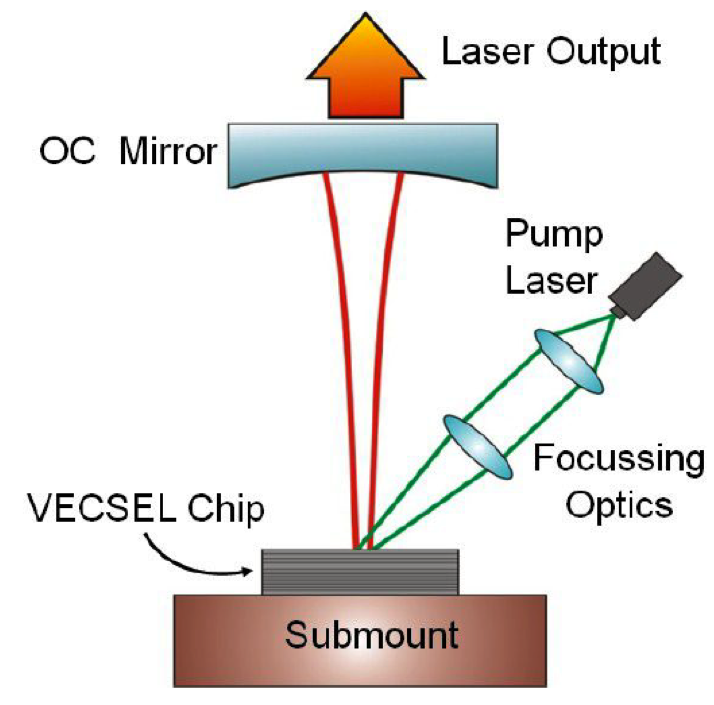
\includegraphics[width=10cm]{img/vecsel_principle.png}
\caption{An optically pumped
vertical-external-cavity
surface-emitting laser
(VECSEL)
is composed of
an output coupler
external mirror (OC)
and the VECSEL chip itself.
The VECSEL chip is composed of
a window layer
(also known as cap),
a gain region,
and a mirror.
It is mounted
on a heat sink,
and pumped
by a diode laser.
From \cite{Sirbu2014SPIE}.}
\label{img:vecsel_principle}
\end{figure}

The active mirror
is composed of
a periodic structure
of quarter wavelength
semiconductor layers;
a distributed Bragg reflector (DBR).
The materials used for the DBR
have to fulfill
three basic requirements
\cite{Calvez2009}.
First of all,
the material has to be transparent,
i.e. non-absorbent,
at the emission wavelength.
Secondly,
the used materials
have to have a high contrast
of refractive index.
This helps to obtain
high reflectivity
with a low number of layers;
smaller devices
have advantageous thermal properties.
Thirdly,
the material used
has to be as thermally conductive as possible.

The gain region
is composed of
quantum wells (QWs).
They are placed
at the antinodes
of the standing-wave
of the optical field
of the design wavelength.
This so-called
resonant periodic gain (RPG)
configuration
helps to avoid spatial hole burning
\cite{Ranta2014OptLett}.
Figure~\ref{img:design}
illustrates our VECSEL chip.

\begin{figure}
\centering
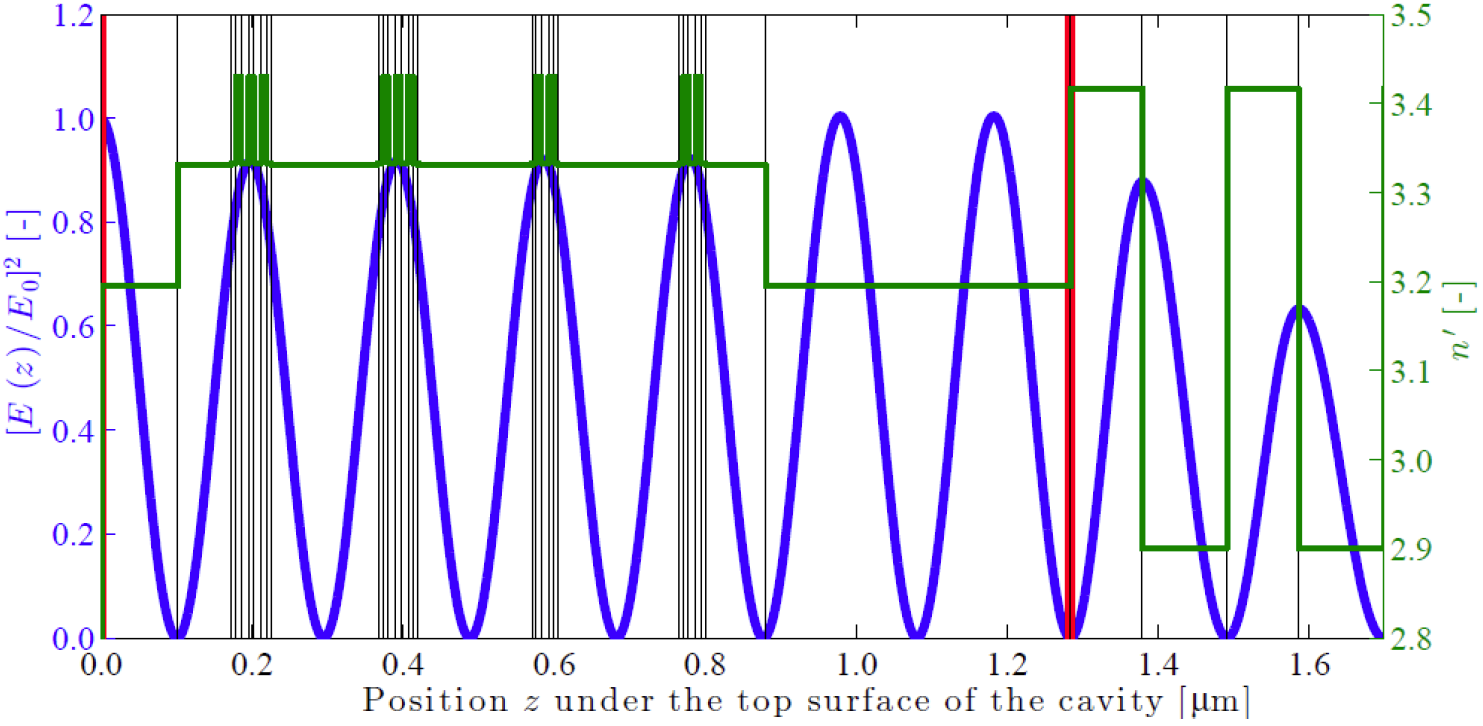
\includegraphics[width=14.5cm]{img/design.png}
\caption{Schematic depiction of our VECSEL structure,
from \cite{Sirbu2014SPIE}.
The first layer from left
is the confinement window
(also known as cap).
It is followed by the
gain region,
up to the red line.
This line indicates
the wafer-fusion interface,
after which follows the DBR.
Only the first two layer pairs
of the DBR
are shown;
there are 24 over all.}
\label{img:design}
\end{figure}

The confinement window
(also known as cap)
is transparent for
pump and signal.
Its function is twofold
\cite{Tropper2006,Calvez2009}.
First,
it is designed to provide
good coupling between
the external and
the sub-cavity.
Secondly,
it is a spacer
to separate the surface
from the carriers
generated in the active region.
This reduces non-radiative recombinations.

The thermal management
is critical for the operation
of VECSELs.
Over the years,
two strategies
for heat extraction
have been established
\cite{Kemp2008,Vetter2012}:
the heat-spreader,
and the thin-disk approach.
In the first strategy
the VECSEL chip is grown
in the order
DBR--gain--cap,
and the heat is extracted
through a chemical vapor deposited
(CVD) diamond
clamped onto the cap.
In the second approach,
the structure is grown
in reverse order,
so the Bragg mirror
can be bonded
onto a CVD diamond.
In this strategy
the heat has to be extracted
through the whole structure.

The heat-spreader approach
tends to be more efficient
to extract the heat --
at least
for relatively small pump spot sizes
\cite{Vetter2012}.
On the down side,
it introduces Fabry-Perot effects,
and makes the device packaging
more bulky over all.
For these reasons
the thin disk approach
would be preferred
for a wide variety
of applications \cite{Ranta2014OptLett}.

\subsection{Wafer-fusion}

With our VECSEL design
we aim to cover
the $1.3\,\mu\mathrm{m}$
wavelength band.
The corresponding material system
for the active region
is InP.
DBRs grown on this material system
do not provide high contrast
in refractive index
and have very low thermal conductivity.
Because of the low contrast,
more layers
are required
in order to obtain
high reflectivity.
And this is unfortunate
for the thermal management,
further aggravated by the low conductivity.
Consequentially,
the highest output powers
in this waveband
were obtained for wafer-fused
devices \cite{Ranta2014OptLett}.
For wafer fusion
the active region
is grown separately
from the DBR
and in a second step
fused along the interface
indicated in Fig.~\ref{img:design}
with red line.

This approach corresponds to
the thin disk strategy
mentioned above.
But it has the additional advantage
to combine material systems
whose design wavelength
is around $1.3\,\mu\mathrm{m}$,
with GaAs-based DBR,
whose contrast in refractive index
and thermal conductivity
allows a more efficient heat extraction.
This property is key
for the high power performance
of wafer-fused devices.
Figure~\ref{img:wafer_fusion}
shows a schematic illustration
of our wafer-fused design.
The DBR is bonded
onto the CVD diamond
using a gold interface.
The DBR-Au bond itself
is realized by employing
titanium as adhesion layer.

Alternatives for
the Au-Au-bonding
involve intermediate In solder.
But this material choice
is disadvantageous
for high temperatures
\cite{Ranta2014OptLett}.
Beside the structural necessities
to use the gold layer,
it is also predicted
to show benefits
for the thermal behavior
and conversion efficiency
of a VECSEL
\cite{Hader2011,Devautour2013}.

The design and
manufacturing process
of the samples
was not within the scope
of this project.
I thus constrain myself
to explain only
the essentials
of these processes
necessary
to understand the report
at hand.
A more detailed description
of the manufacturing process
is given in \cite{Ranta2014OptLett,Sirbu2014SPIE}.

\begin{figure}
\centering
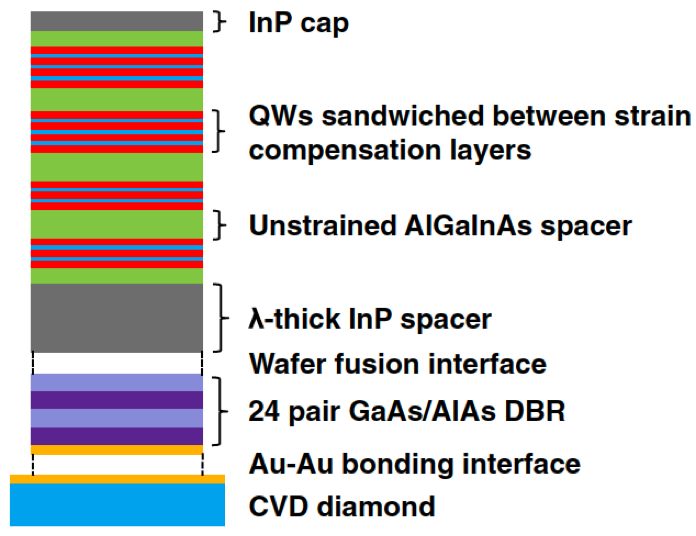
\includegraphics[width=8cm]{img/wafer_fusion.png}
\caption{Our InP-based VECSEL design
incorporating AlGaInAs quantum wells (QWs),
wafer-fused,
and bonded on CVD diamond.
The $\lambda$-thick InP spacer
acts as a defect blocking layer.
The gain region was grown
by metallorganic vapor phase epitaxy (MOVPE),
the DBR was grown
by molecular beam epitaxy (MBE).
From \cite{Ranta2014OptLett,Sirbu2014SPIE}.}
\label{img:wafer_fusion}
\end{figure}

\section{Thermal resistance}
\label{sec:rth}

The thermal resistance ($\Rth$) is
the only experimentally accessible quantity
to asses the heat flow
in the structure \cite{Heinen2012}.
The thermal management
of a VECSEL is of critical importance
\cite{Tropper2006,Kemp2008,Vetter2012,Giet2008}.
Consequentially,
we're interested to determine $\Rth$.
It is a useful
figure of merit
to keep track of improvements
on design and manufacturing process
of VECSEL technology.
The thermal resistance
describes how much the sample heats up ($\d T$)
as a result of the dissipated power $\d D$
\begin{equation}
\d T = \Rth \d D \quad \Rightarrow \quad \Rth = \pd{T}{D}.
\label{eq:rth}
\end{equation}

There are several methods deployed
to determine
the thermal resistance,
an overview can be found in \cite{Heinen2012}.
Most of them are time and equipment intensive.
This is impractical
in order to monitor
improvements made in a design and
manufacturing process.
More simple approaches are desired.
For this report
I review two methods
that are supposed to be
just that.


\subsection{By spectral shift}
\label{sec:rth:lambda}

We can write the thermal resistance from (\ref{eq:rth})
as \cite{Heinen2012,Giet2008}
\begin{equation}
\Rth = \pd{T}{D} = \pd{\lambda}{D}/\pd{\lambda}{T}.
\label{eq:rth_long}
\end{equation}
In this description
$\lambda$ corresponds to
the longest emitted wavelength.
The longest emitted wavelength is said to
correspond to the hottest part of the VECSEL.
This is a result of the predominantly linear shift
in refractive index
as function of temperature \cite{Heinen2012}.
This approach ignores
the change in cavity length
resulting from thermal expansion.

The longest emitted wavelength
is correlated
with dissipated power.
This gives a linear relation
for each heat sink temperature
\begin{equation}
\lambda_{\Ths} = \left.\pd{\lambda}{D}\right|_{\Ths} D + \lambda_{0,\Ths}.
\end{equation}
By substituting
\begin{equation}
\lambda_{0,\Ths} = \pd{\lambda}{T} \Ths + \lambda_0
\end{equation}
we end up with \cite{Heinen2012}
\begin{equation}
\lambda = \pd{\lambda}{D} D + \pd{\lambda}{T} \Ths + \lambda_0,
\label{eq:rth_fit}
\end{equation}
from where we can extract
the required parameters for (\ref{eq:rth_long})
using linear regression.

We record the emitted spectrum
for every pump setting.
In order to determine
the longest emitted wavelength
we cut
these spectra
as indicated
in Fig.~\ref{img:longest_wavelength}.
By measuring each pump setting multiple times,
we can increase our confidence
in the extracted wavelength value.

\begin{figure}
\centering
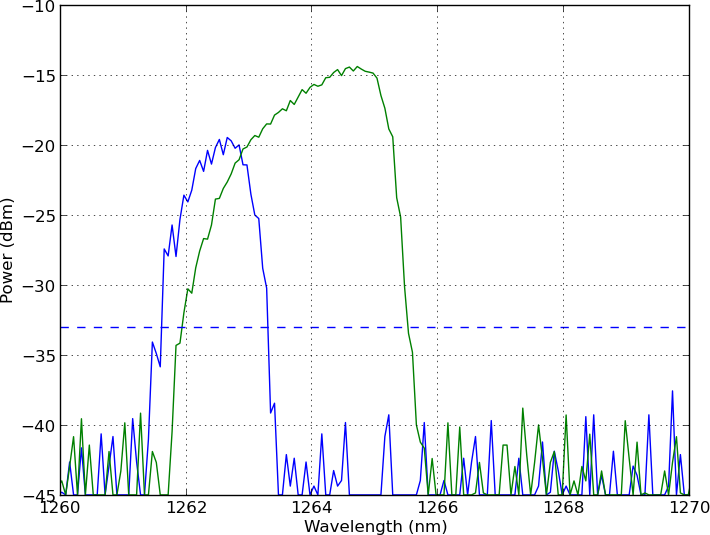
\includegraphics[width=10cm]{img/longest_wavelength.png}
\caption{We cut the spectrum
at a level
above the noise floor.
For each pump setting
we have multiple measurements,
giving us a margin
of how reliable this extracted
longest wavelength is.}
\label{img:longest_wavelength}
\end{figure}

The dissipated power $D$
corresponds to the left-over power
of the pump ($P$),
after we have accounted for the
reflected ($R$) and emitted ($E$) part
\cite{Heinen2012},
\begin{equation}
D = P - R - E.
\label{eq:dissip}
\end{equation}
\subsection{By roll over}
\label{sec:rth:trollover}

A second method,
relies on an intrinsic roll over temperature.
Roll over is an effect due to the optical pumping:
While increasing the pump power
in order to obtain higher emitted output,
we heat the gain structure.
This increase in temperature
introduces an additional loss
which the gain
has to compensate.
Otherwise,
our device stops lasing.
After a certain point
the gain cannot compensate for the losses anymore,
and this region stops contributing
to the output.
We see
a decline
in output power
despite the higher pump --
a roll-over.

Heinen et al. \cite{Heinen2012}
have found empirically --
using the method described in \ref{sec:rth:lambda} --
the longest wavelength
at this roll over point
is the same wavelength,
regardless of the heat sink temperature.
They conclude,
this wavelength to correspond
to an of the structure intrinsic
critical temperature --
the roll over temperature.
Given definition (\ref{eq:rth})
we find
the difference in temperature
between (unknown) roll over and heat sink.
It is
the thermal resistance
times the dissipated power,
\begin{equation}
T_\mathrm{ro} - \Ths = \Rth D_\mathrm{ro}.
\end{equation}
In other words,
when we plot
dissipated power at roll over ($D_\mathrm{ro}$)
versus the heat sink temperature
for this measurement $\Ths$,
we find a linear relation.
Its slope corresponds
to the thermal resistance,
and the $y$-intersection
to the roll over temperature \cite{Heinen2012}:
\begin{equation}
\Ths = -\Rth D_\mathrm{ro} + T_\mathrm{ro}.
\end{equation}

This relation is wavelength independent.
Mode instabilities in pump and emission
are expected to result in fluctuations
in the emitted spectra.
A spectrum independent method
to determine $\Rth$ is thus supposed to
yield a result with smaller uncertainty.
The difficulties in this second method
arise from identifying
the exact point of roll over.
Whether this identification
is more or less error-prone
is open for discussion.
Furthermore,
it is not yet clear
whether all VECSEL designs
show this intrinsic roll over behavior.
\subsection{Remarks on experimental access and corrections}

Hader et al. \cite{Hader2013}
have pointed out,
the used definition of
dissipated power (\ref{eq:dissip})
ignores a relevant loss channel.
Namely,
beside the reflected,
emitted,
and dissipated part
there are additional non-heating losses
the incident pump converts into.
These additional losses come from
non-heating spontaneous emission
and surface-scattering.
Without these
we overestimate $\Rth$.
The losses due to surface-scattering
are particularly pronounced
when using an output coupler
with low out-coupling losses.

From a theoretical point of view
the comments made by
Hader et al. \cite{Hader2013}
may be relevant.
However, for the experimental approach
they're impractical
as the invoked calibration
is tedious.
Especially,
if the main objective in monitoring $\Rth$
is to obtain a figure of merit
for the thermal management
of the VECSEL structure.
As a remedy,
Hader et al. suggest
using an output coupler
with higher out-coupling losses.
The scattering losses
would be less pronounced.
In this report,
I ignore these additional effects
and work with (\ref{eq:dissip}).
Consequentially,
the stated values for the determined $\Rth$'s
are likely to overestimate
the true value.
\subsection{Power-scalability}
\label{sec:rth:scaling}

The gain section of a VECSEL
is very thin compared to
the dimensions of the optical pump spot.
This gain region
is heated
due to the difference in photon energy of pump and output
and due to non-radiative recombinations.
In other words,
heat is extracted
over a short path
with respect to the pump spot size,
and the resulting
heat flow is
approximatively one dimensional.
Lateral cooling is
therefore
not as relevant
for the operation of such a device.
One dimensional heat extraction means
the device is power scalable:
increasing the pumped area
does not introduce
significantly additional heating.
The output power
can be enhanced
by enlarging the pumped area,
so more of the gain material
is stimulated
into emission.
This is the expected behavior
of disk lasers.
\cite{Tropper2006,Lindberg2005,Le1991}.

Several effects
hinder the real device
to live up to these expectations.
Bedford et al. \cite{Bedford2005} report
a limit to this scalability:
there is a critical diameter
above which amplified spontaneous emission (ASE)
and lateral lasing
become relevant.
These effects introduce additional losses
which inevitably limit the output scaling.
The pump beam shape
was found to
limit the power scaling further \cite{Chernikov2010}.
Furthermore,
larger beam spots
risk to be more susceptible
to surface impurities
and non-radiative defects \cite{Korpi2010}.

If the thermal resistance $\Rth$
were to power scale,
its value would have to decrease
at an inverse rate of the pumped area, $w^{-2}$.
As discussed by Giet et al. \cite{Giet2008},
this is not the case.
Instead,
the decrease in $\Rth$ follows more closely
the radius (diameter) of the pump spot
than the area, $w^{-1}$.
This behavior is apparent when we plot
spot size versus thermal resistance
in a log-log plot.
The slope in such a plot
is closer to $-1$ than to $-2$.

For the sake of completeness,
the thermal resistance can be fitted with
the empirical formula \cite{Giet2008}
\begin{equation}
\Rth(w) = a_1+ \frac{a_2}{w} \left( 1-\frac{w}{a_3} \right)^{1.5}.
\label{eq:Rth_empirical}
\end{equation}
This formula was adopted
form a fit originally developed for VCSELs \cite{Nakwaski1992}.
In the original form
the ratio within the brackets
represented the ratio between an inner and outer diameter
of the VCSEL.
Working with VECSELs we lack such a definition.
As such,
it is not clear
what parameters $a_{\{1,2,3\}}$ are supposed
to tell us about the VECSEL under test.
So far,
this description is not yet widely used
by the scientific community.



\section{Surface temperature raise, numerically}
\label{sec:comsol}

The commercial software COMSOL
allows us to perform thermal simulations
with a finite-element approach.
The heat equation
to be solved
reads as
\begin{equation}
0 = \nabla(k\nabla T) + Q.
\label{eq:heateq}
\end{equation}
It is $k$ the thermal conductivity of the material
($[k]=\mathrm{m}^{-1}$),
and $Q$ the heat source
($[Q]=\mathrm{W}/\mathrm{m}^3$);
originating from the pump beam.
With this equation we take into account
only conduction
and ignore convection.
In anisotropic materials
the thermal conductivity differs
depending on the direction of conduction.
For the simulation we assume radial symmetry,
in order to bring the 3D problem down to 2D.
This saves computation time.

In this section,
I cover some numerical considerations
regarding the pump induced
temperature increase
within the different layers
of a VECSEL structure.
The presented plots
show the expected temperature profile
along the most important interface:
the top of the gain section \cite{Ranta2014OptLett}.

I only describe
the new considerations
made in the course
of this project.
While in appendix~\ref{app:comsol_deriv},
I explain
where the formulae come from
that are widely used in literature
\cite{Ranta2014OptLett,Kemp2008,Kemp2005,Vetter2012,Lindberg2005}.
This appendix also provides
additional insights,
necessary to properly implement
our structure in COMSOL.
I start by introducing
a beam profile
that was so far not considered
in these investigations.
Eventually,
I present
the calculated
pump induced temperature increase
along the surface of the gain layer
of our VECSEL structure,
considering different pump powers
and pump beam profiles.



\subsection{Pump beam profile}
\label{sec:comsol:beamprofile}

For the heat source $Q$
in (\ref{eq:heateq})
we assume
the pump beam
is incident antiparallel to the $z$-axis
(here referred to as from the top),
and of Gaussian profile.
In this orientation the heat source
associated with
each layer $j$ of the structure is given as
\cite{Kemp2008}
\begin{equation}
Q_j = \frac{2P}{\pi w^2} \eta_j\alpha_j \e^\frac{-2r^2}{w^2} \e^{-\alpha_j(z_{0j}-z)} \e^{-\sum_{i<j}\alpha_i t_i}.
\label{eq:heatsrc}
\end{equation}
This representation counts the layers
from the top down --
the sum $\sum_{i<j}$ includes the layers on top
and ignores those below the layer of interest
(in that case $j$).
A derivation,
as well as a more in-depth explanation
what the different parameters stand for,
is given in
appendix~\ref{app:comsol_deriv:Q}.

Equation (\ref{eq:heatsrc})
describes a Gaussian pump profile
by design.
In reality, however,
the pump profile is most likely not Gaussian.
In fact,
the pump spot imaged from a multimode fiber
resembles a flat-top
(also known as top-hat)
distribution \cite{Tropper2006},
or at least a super-Gaussian
\cite{Chernikov2010,Heinen2012el}.
Figure~\ref{img:visuallize_sGauss}
illustrates the difference in beam shape
of these mentioned three types.

In order to incorporate
a flat-top pump profile,
we have to replace the Gaussian part
in (\ref{eq:heatsrc}) \cite{Kemp2005}:
\begin{equation}
2\e^\frac{-2r^2}{w^2} \to
\left\{
\begin{matrix}
1 & r\leq w \\
0 & r>w.\\
\end{matrix}
\right.
\label{eq:replflattop}
\end{equation}
This can easily be verified as the renormalization has to match,
\begin{equation}
\frac{2}{w^2} \int\limits_0^\infty r \d r \e^\frac{-2r^2}{w^2}
= \frac{1}{w^2} \int\limits_0^w r \d r = \frac{1}{2}.
\label{eq:heatsrc_renorm}
\end{equation}

A super-Gaussian is of the form \cite{Chernikov2010}
\begin{equation}
f(x) \propto \e^{-|\frac{x}{w}|^\beta}.
\label{eq:super-gauss}
\end{equation}
The Gaussian profile (\ref{eq:gaussE})
corresponds to the special case $\beta=2$,
and the flat-top distribution to $\beta=\infty$.
Parameter $w$ corresponds
to the $\e^{-2}$ radius
\begin{equation}
w = \frac{\mathrm{FWHM}}{2(\frac{1}{2}\log2)^{1/\beta}}.
\end{equation}
This definition of $w$ is necessary
in order to be compatible
with the definition
of the flat-top distribution
already known in literature
\cite{Kemp2005}.
However,
in \cite{Heinen2012el}
they measured the profile
of their super-Gaussian pump,
and decided to report
the FWHM
as spot diameter.

Before we can incorporate a super-Gaussian,
we have to numerically find the normalization factor
\begin{equation}
a_p = \frac{2}{w^2} \int\limits_0^\infty r \d r \e^{-2|\frac{r}{w}|^\beta}.
\label{eq:super-gauss-scaling}
\end{equation}
Analogously to (\ref{eq:replflattop}),
for a super-Gaussian profile
we replace in (\ref{eq:heatsrc})
\begin{equation}
2\e^\frac{-2r^2}{w^2} \to \frac{1}{a_p}\e^{-2|\frac{r}{w}|^\beta}.
\label{eq:replsupergauss}
\end{equation}
Four examples for the normalization factor,
rounded to four digits, are
$a_{2}=0.5$,
$a_{3}=0.5687$,
$a_{4}=0.6267$,
and $a_\infty=0.5$.
See also
the analytic results in (\ref{eq:heatsrc_renorm}),
and Fig.~\ref{img:visuallize_sGauss}.

\begin{figure}
\centering
\subfigure{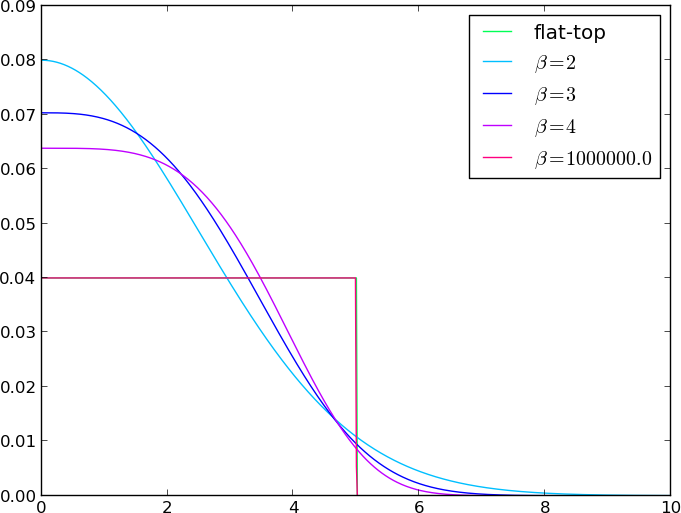
\includegraphics[width=7cm]{img/visuallize_super-Gauss_f2.png}}
\subfigure{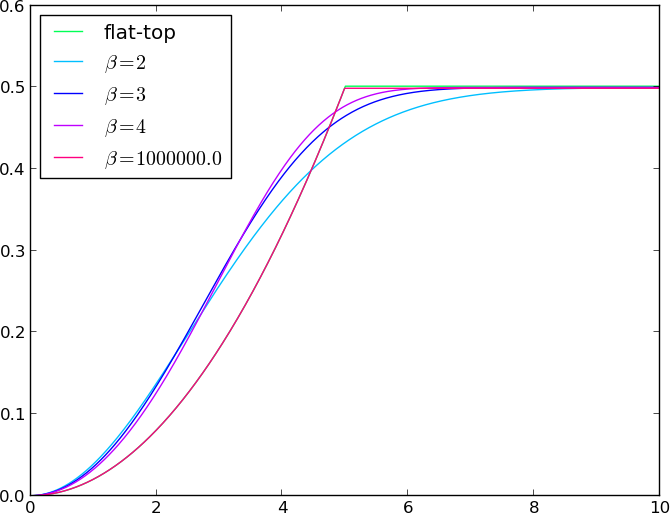
\includegraphics[width=7cm]{img/visuallize_super-Gauss_f2int.png}}
\caption{A super-Gaussian of the form
$f^2(x) \propto \e^{-2|x/w|^\beta}$
\cite{Chernikov2010}
describes an intermediate shape
between a regular Gaussian with $\beta=2$
and flat-top with $\beta=\infty$.
Left,
we see the squared shapes
of super-Gaussians $f^2(x)$ with $w=5$
for different values of $\beta$,
including flat-top as a point of reference.
The normalization is chosen such that
the over all integral corresponds to $0.5$;
from (\ref{eq:heatsrc_renorm}).
This is demonstrated in the plot to the right.}
\label{img:visuallize_sGauss}
\end{figure}
\subsection{Pump profile dependent temperature increase on gain surface}

With the concepts described in
appendix~\ref{app:comsol_deriv}
and section~\ref{sec:comsol:beamprofile}
we can look at
the expected temperature increase
of our structure,
corresponding to different pump beam profiles.
The thermal load
inflicted on the structure
depends on this pump distribution.
The image of a multi-mode fiber
can be described by a super-Gaussian.
This category describes
a generalized Gaussian profile
of the form $f(x)\sim\e^{-|\frac{x}{w}|^\beta}$
\cite{Chernikov2010},
see Fig.~\ref{img:visuallize_sGauss}.
It covers
distributions between
Gaussian ($\beta=2$) and flat-top ($\beta=\infty$).
The closer the pump beam distribution
resembles a flat-top distribution,
the more evenly the temperature load
is distributed.

The numerical analysis
for super-Gaussian profiles
is particularly interesting:
while the temperature profile
caused by Gaussian and flat-top distributions
were already reported \cite{Kemp2005},
the intermediate super-Gaussian profile
was ignored thus far.
The fact that
the pump profile
is relevant
for the performance of VECSELs
was demonstrated in \cite{Chernikov2010}.

We can assume roll over occurs
once the gain material exceeds
a critical temperature \cite{Heinen2012},
see section~\ref{sec:rth}.
In order to postpone
the critical pump power
to higher values,
we have to lower the peak temperature
invoked by the pump.
Figure~\ref{img:Comsol_Tvsr} shows,
this can be achieved
by either assuming
a super-Gaussian beam profile
or a regular Gaussian
with larger spot size.

\begin{figure}
\centering
\subfigure{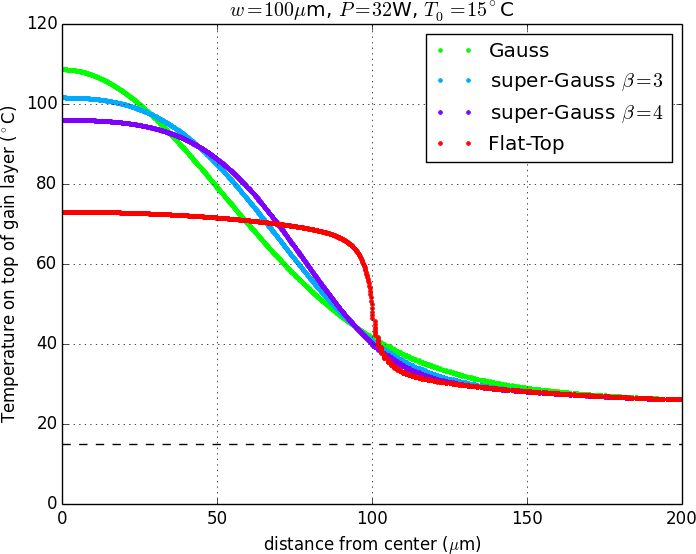
\includegraphics[width=7cm]{img/Comsol_Tvsr_32W_100um.png}}
\subfigure{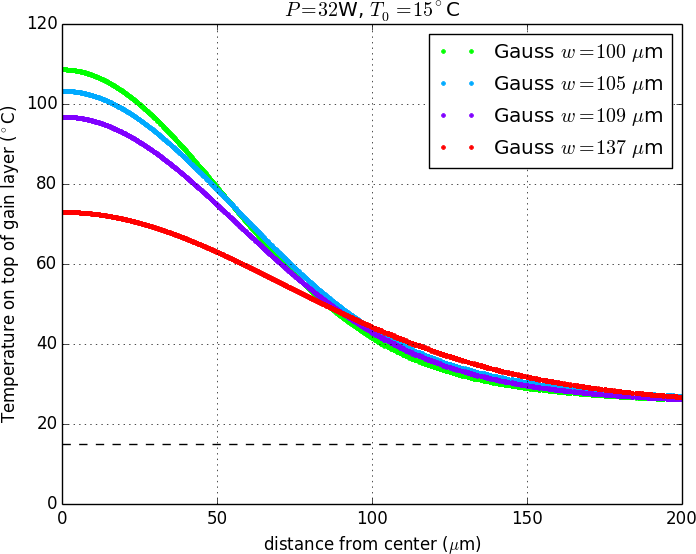
\includegraphics[width=7cm]{img/Comsol_Tvsr_32W_sG-equivs.png}}
\caption{Temperature along surface of the gain section, $z_\mathrm{0g}$
(Tab.~\ref{tab:comsolparams}).
The different beam shapes from Fig.~\ref{img:visuallize_sGauss}
with the same total power
induce a different increase in temperature
with respect to $T_0$,
indicated by the dashed line (left).
The same peak temperature can be found
employing regular Gaussians
with larger beam spots.
These however,
have a larger fraction
of the power distribution
below threshold
in the tail region,
which contributes only to heating
but no light emission.}
\label{img:Comsol_Tvsr}
\end{figure}

The peak temperature
is not the only relevant quantity
for an efficient pump profile:
the gain needs to be irradiated
with enough power
to transcend threshold.
The regions of the sample
irradiated by pump light
but below threshold
do not contribute to the laser output.
However, these regions do heat the structure.

The stronger we pump,
the larger the area on the sample
irradiated by above-threshold power.
This above-threshold
region corresponds to
the relevant, effective area.
In the case of the accentuated Gaussian beam,
the center exceeds
the roll over temperature
at a relatively low pump power,
while the effective area
is still relatively small.
In contrast,
a super-Gaussian pump profile
is capable activating
a larger effective area,
while at the same time
lowering the peak temperature.
Consequentially,
roll over is expected
to occur at higher pump power.

These simulations demonstrate
the thermal management
depends on the pump profile.
Furthermore, they suggest
a Gaussian pump profile
to be non-ideal
concerning the inflicted thermal load.
This reasoning is consistent
with the findings in \cite{Chernikov2010}.

This provokes
me to issue a warning:
extracting thermal resistance $\Rth$
only for the hottest spot,
as suggested in section~\ref{sec:rth},
does not tell the full story.
We can find normal Gaussians
with the same peak temperature
as super-Gaussians,
Fig.~\ref{img:Comsol_Tmax_BeamProfile}.
Comparing thus extracted values of $\Rth$
with values measured with other setups --
and expectedly different pump profiles --
is hence not valid.

\begin{figure}
\centering
\subfigure{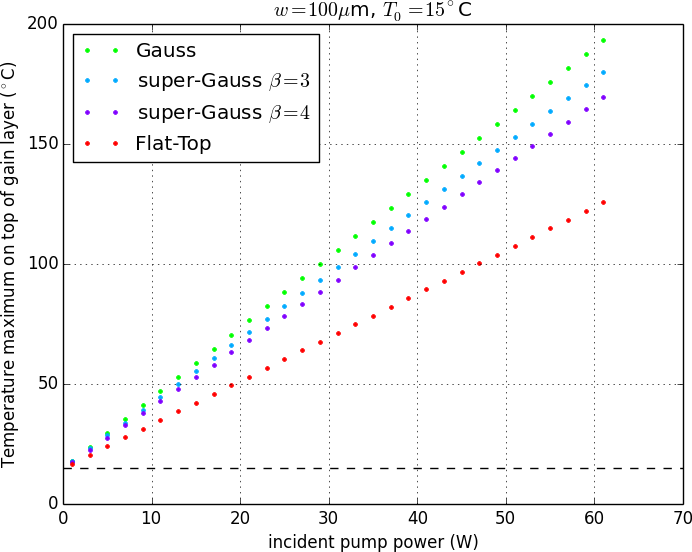
\includegraphics[width=7cm]{img/Comsol_Tmax_BeamProfile_32W_100um.png}}
\subfigure{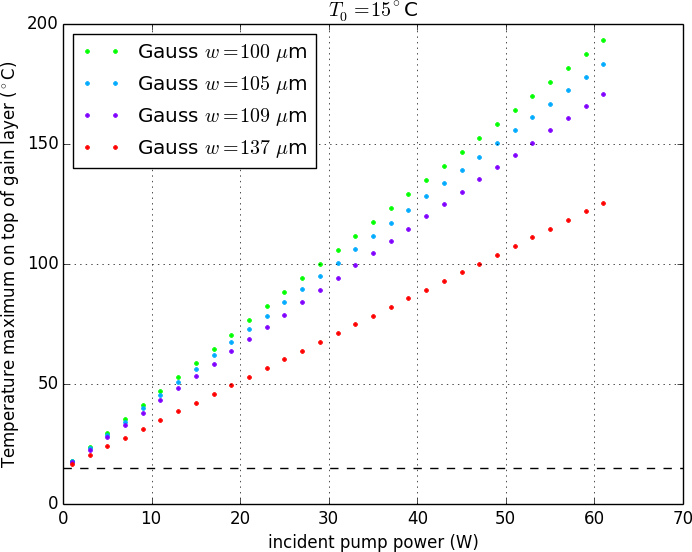
\includegraphics[width=7cm]{img/Comsol_Tmax_BeamProfile_32W_sG-equiv.png}}
\caption{The maximum temperature (i.e. at $r=0\,\mu\mathrm{m}$)
of the different beam profile depicted in Fig.~\ref{img:Comsol_Tvsr},
for various settings of total power.
The increase in peak temperature
does not change qualitatively
whether we consider super-Gaussians (left)
or regular Gaussians with larger radii (right).}
\label{img:Comsol_Tmax_BeamProfile}
\end{figure}





\section{Experimental Setup}
\label{sec:exp}

The main objective
is to look at the high power regime,
attractive for intra-cavity frequency mixing.
For this,
I report on the light-light performance
of $1270\,\mathrm{nm}$ waveband VECSELs
with wafer fused gain mirrors
set in the flip-chip heat dissipation scheme,
see section~\ref{sec:basics}.
The light-light characteristics
relates the pumped input power
with the converted
emission power.
is recorded for various heat sink temperatures.
To asses the thermal management
we determine the thermal resistance
of our device.
Following section \ref{sec:rth},
we have to keep track of
the pumped,
reflected,
and emitted power,
and the emitted spectra.

\subsection{Setup and sample}
\label{sec:exp:setup}

\begin{figure}
\centering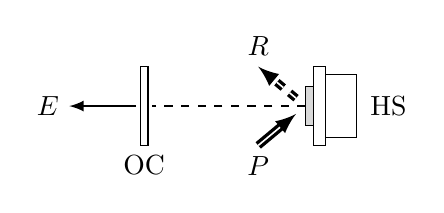
\begin{tikzpicture}[>=latex]
    %%%%%%%%%%%%%%%%%%%%%%%%%%%%
    % requires libraries:
    % \usetikzlibrary{arrows,decorations.pathmorphing,backgrounds}
    %%%%%%%%%%%%%%%%%%%%%%%%%%%%
    \begin{scope}[xshift=0cm]
    % sample holder
    \draw (0.25,0.1) rectangle (0.65,.9);
    \node[right] at (0.7,0.5) {HS};
    \draw (0.1,0) rectangle (0.25,1);
    \filldraw[fill=gray!30] (0,0.25) rectangle (0.1,0.75);

    % pump
    \draw[->,very thick,double] (-0.6,0) -- (-0.12,0.4)
        node[pos=0,below] {$P$};
    \draw[->,very thick, double, dashed] (-0.12,0.6) -- (-0.6,1)
        node[pos=1,above] {$R$};

    %laser
    \draw[thick,dashed] (0,0.5) -- (-1.95,0.5);
    \draw[->,thick] (-2.15,0.5) -- (-3,0.5)
        node[pos=1,left] {$E$};

    \draw (-2,0) rectangle (-2.1,1);
    \node[below] at (-2.05,0) {OC};
    \end{scope}

\end{tikzpicture}

\caption{The sample is mounted on a
water cooled heat sink (HS).
The external cavity is defined by the output coupler (OC)
and the active mirror
attached to the HS.
The pump is incident at
approximately $36\,^\circ$, with power $P$.
We are further interested in
the emitted power $E$,
and the reflected power $R$.}
\label{img:setup_sketch}
\end{figure}

Figure~\ref{img:setup_sketch} depicts
the basic scheme of the used setup:
The VECSEL sample is mounted
on a water cooled heat sink,
and is optically pumped by power $P$,
with a pump spot size
of radius $w$.
Some of this pump light is
converted and emitted ($E$),
reflected off the sample ($R$),
and the rest is said to be dissipated ($D$),
through the sample
onto the heat sink.
For the light-light characteristics
we are interested
in the relation between $P$ and $E$.
Respectively,
we are interested in
how much of the net pump light
is converted into emitted light.
This net pump we signify as
absorbed power
\begin{equation}
A = P-R.
\label{eq:abspwr}
\end{equation}
This definition
of absorbed power
overestimates
the real absorbed power,
it ignores
surface scattering and
spontaneous emission outside the cavity.
For the experiments
presented this report,
I ignore these loss channels.

The pump is a $980\,\mathrm{nm}$ diode laser.
Figure~\ref{img:pumpspectrum} illustrates the spectrum
for two different pump currents.
The pump is delivered by a multimode fiber.
We image its end onto the sample,
under an incidence angle
of approximately $36\,^\circ$,
using various lenses.
This results in
the various spot diameters
$2w=\{180,200,300,333,400,444\}\,\mu\mathrm{m}$.
To ensure good mode overlap
the cavity lengths has to be adjusted.

\begin{figure}
\centering
\subfigure{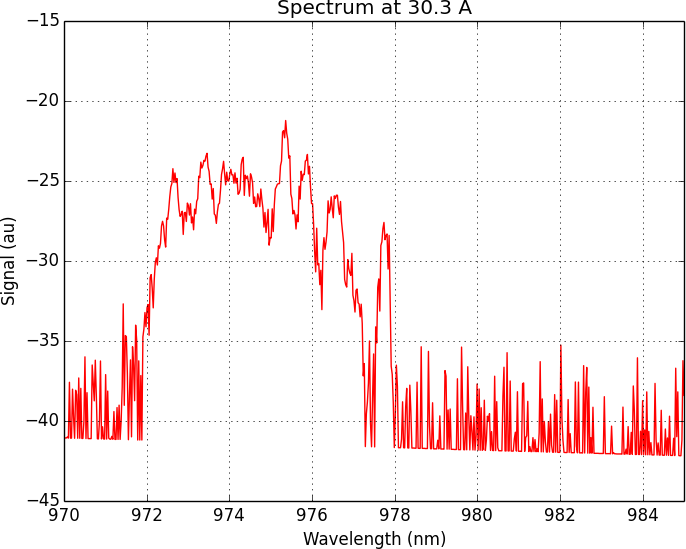
\includegraphics[width=7cm]{img/PumpSpectrum30p3A.png}}
\subfigure{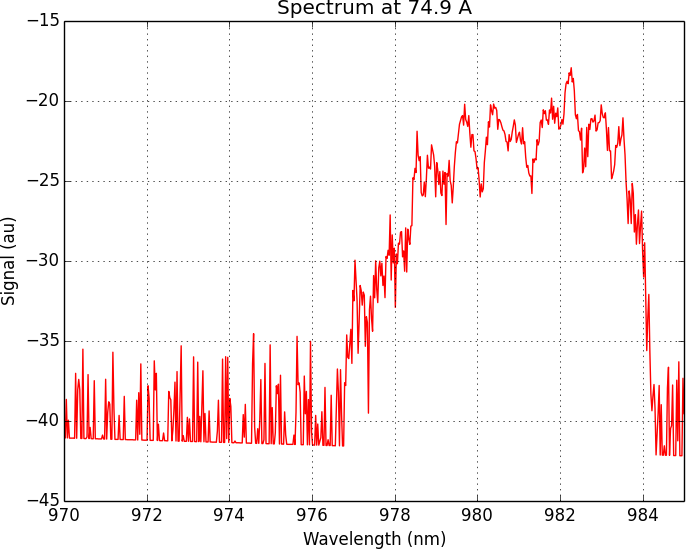
\includegraphics[width=7cm]{img/PumpSpectrum74p9A.png}}
\caption{Spectrum of nominally $980\,\mathrm{nm}$ pump beam;
measured at $\approx6\,\mathrm{cm}$ distance to
divergent pump delivery fiber,
under $0\,^\circ$ incidence.
The plots correspond to an optical output of
$21\,\mathrm{W}$ and $56\,\mathrm{W}$,
respectively.}
\label{img:pumpspectrum}
\end{figure}

The VECSEL-sample is designed to emit
around $1270\,\mathrm{nm}$.
The fabrication details are published elsewhere
\cite{Ranta2014OptLett,Sirbu2014SPIE};
they are not part of this report.
The essential details are highlighted
in section~\ref{sec:basics},
section~\ref{sec:intro}.

Monitoring the reflection
off the sample
is crucial for high power operation.
For one,
we want to design the VECSEL structure
such that it absorbs as much
of the pump light as possible.
Secondly, depending on the exact application
the VECSEL is used for,
the reflected light may pose
a health hazard;
or at least an additional heat spot
that needs to be taken care of.

The thermal resistance $\Rth$
connects the sample temperature
with the dissipated power (\ref{eq:rth})
\begin{equation}
T = \Rth D.
\end{equation}
The performance of a VECSEL depends on temperature.
The thermal management of the device is thus critical
\cite{Tropper2006,Kemp2008,Vetter2012}
and thus a low thermal resistance is desired.
Furthermore,
the thermal resistance
is the only experimentally accessible quantity
to assess the heat flow in a VECSEL \cite{Heinen2012}.
Beside the quantities mentioned in Fig.~\ref{img:setup_sketch},
in order to estimate the thermal resistance
we also need to record the spectrum of the emitted light
\cite{Ranta2014OptLett,Heinen2012},
see section~\ref{sec:rth}.

Figure~\ref{img:setup_photo} shows a photograph of our setup.
It meets the specifications
to measure pumped,
reflected, and
emitted power,
as well as the spectra
simultaneously.
The pumped and reflected power
we measure by sampling
a fraction of the beam.
The reflectivity of these beam sampler
depend on the incidence angle.
This beam sampling fraction
needs thus to be recalibrated
whenever we change the beam sampler configuration.
We have to adjust the configuration
for example when we change
the pump spot size.

The pump spot size we vary
by changing the lenses
used to image the fiber end
onto the sample.
In Fig.~\ref{img:setup_photo}
these are denoted as
$\mathrm{L}_\mathrm{p1}$ and $\mathrm{L}_\mathrm{p2}$.
The distance between delivery fiber
and the first lens has to
correspond to its focal length.
In this configuration
the beam after the first lens is collimated.
This arrangement we test by eye,
with the help of an IR-viewer.
The pump spot is at
a distance of a focal length
after the second lens.

In order to find the exact distance,
we look for the alignment
with the lowest lasing threshold --
visualized by a camera
in the emission path.
This initial position
is further optimized
during the fine-alignment
of the output coupler,
aiming at optimal output power.
 
The ratio in focal lengths
of the two employed lenses
corresponds to obtained spot size.
I report the usage
of two types of lenses
for lens $\mathrm{L}_\mathrm{p1}$:
a plano-convex,
spherical lens
motivated by the publications
by Heinen et al. \cite{Heinen2012el,Heinen2012};
and a plano-convex, achromatic lens.
Given the fairly narrow pump spectrum
depicted in Fig.~\ref{img:pumpspectrum}
we wouldn't expect
the achromaticity itself
to have much of an effect.
On the other hand,
the achromatic doublet
has been corrected
for various aberrations \cite{ThorlabsAC}.
This may contribute
a relevant beam property.
All lenses,
as well as the beam samplers,
are appropriately coated
(meaning B- and C-coated
in the pump and emission branch,
respectively).

\begin{figure}
\centering
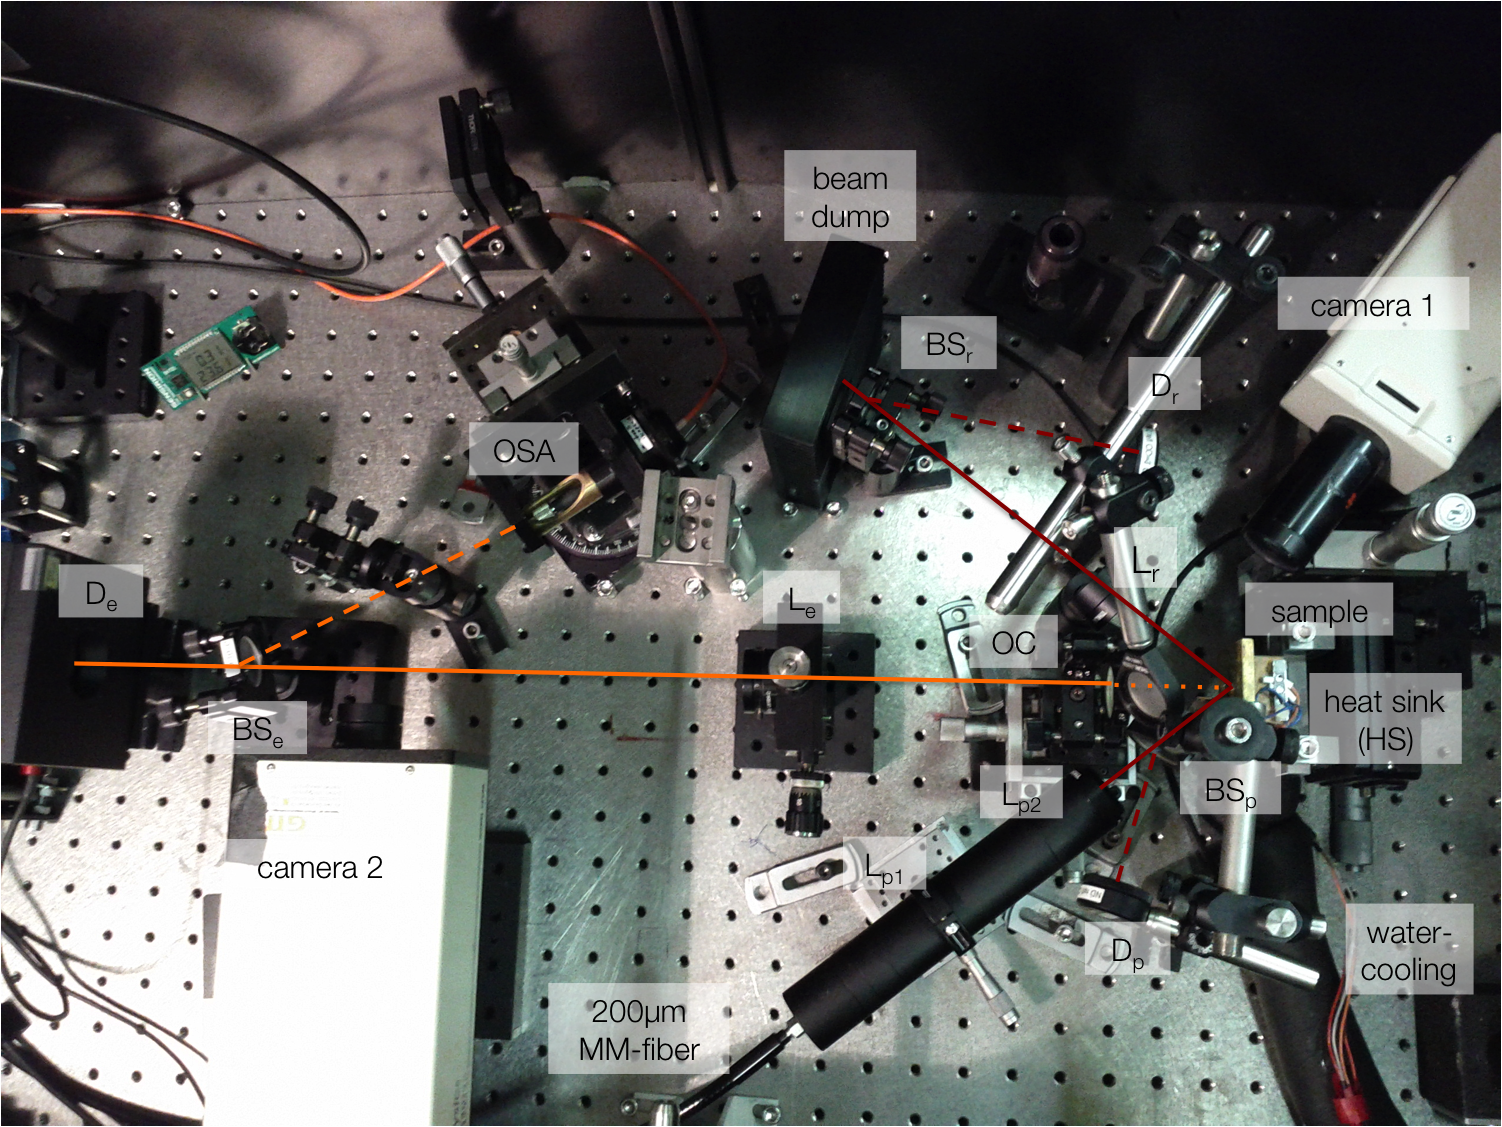
\includegraphics[width=14.5cm]{img/setup_photo.png}
\caption{The pump light is delivered
with a $200\,\mu\mathrm{m}$ multimode (MM) fiber
whose end is imaged onto the sample.
The sample is
mounted on a water cooled copper heat sink.
We image
using various lenses
($\mathrm{L}_\mathrm{p1}$,$\mathrm{L}_\mathrm{p2}$),
resulting in various spot sizes.
The reflected, divergent light
is collected by lens $\mathrm{L}_\mathrm{r}$
and subsequently directed onto a beam dump.
The two beam sampler
($\mathrm{BS}_\mathrm{p}$ and $\mathrm{BS}_\mathrm{r}$)
probe a fraction of the pumped
and reflected light.
This beam sample is directed
to their respective detectors
($\mathrm{D}_\mathrm{p}$ and $\mathrm{D}_\mathrm{r}$).
The sample,
together with the output coupler (OC),
form the external cavity.
The OC has an output coupling loss
$\alpha_\mathrm{OC}=2.5\,\%$,
and a radius of curvature
$ROC=50\,\mathrm{mm}$.
The VECSEL emission
is collected by lens $\mathrm{L}_\mathrm{e}$
and directed onto power meter $\mathrm{D}_\mathrm{e}$.
A fraction of this output
is extracted by beam sampler $\mathrm{BS}_\mathrm{e}$
and directed onto the MM-fiber
connected with the optical spectrum analyzer (OSA).
The polarization
of neither
pump nor emission
is filtered,
in our setup
we do not distinguish
between polarization dependent phenomena.
Cameras 1 and 2 facilitate the alignment.}
\label{img:setup_photo}
\end{figure}

The sample is attached on a ceramic plate,
which itself is attached
to a water cooled copper block,
using thermal grease.
The reported heat sink temperature
is the temperature we measure
at the copper block.
Due to the irradiated power
the heat sink cannot keep a constant temperature.
As a result the measurements
see a fluctuation of about
$\pm$\degr{1} standard deviation.
These temperature fluctuations are addressed
again in subsection~\ref{sec:exp:measroutine}.

I have worked with
two samples,
addressing a proposed optimization strategy
\cite{Hader2011}.
A magnified photo of
sample 1 is shown in Fig.~\ref{img:sample_surface}.
It is illuminated by $980\,\mathrm{nm}$ pump light,
highlighting the defects
that don't contribute to photo luminescence.
The camera has burnt spots itself.
In order not to confuse
the camera defects
with those of the structure,
I have covered those of the camera
with blue dots.
The presented measurements
were taken when irradiating
either of the two regions
denoted as A and B,
respectively.

We investigate the effect
of two optimization strategies
\cite{Hader2011}.
First, we have coated this same sample 1
with an anti-reflection coating.
The surface integrity
after the necessary
surface treatment
and coating
is shown in Fig.~\ref{img:sampleAR_surface}.
It doesn't highlight the surface roughness
which visibly worsened
because of the coating.
This lead to poorer performance,
as will be discussed
in section~\ref{sec:eval:maxout}.

For the second optimization
the gold layer between the DBR
and the CVD diamond
is treated to be highly reflective.
For this measure
we have to take a second sample.
Its active region and DBR
are identical
with those of sample 1.
Figure~\ref{img:sampled6_surface}
shows the surface integrity
of sample 2.

\begin{figure}
\centering
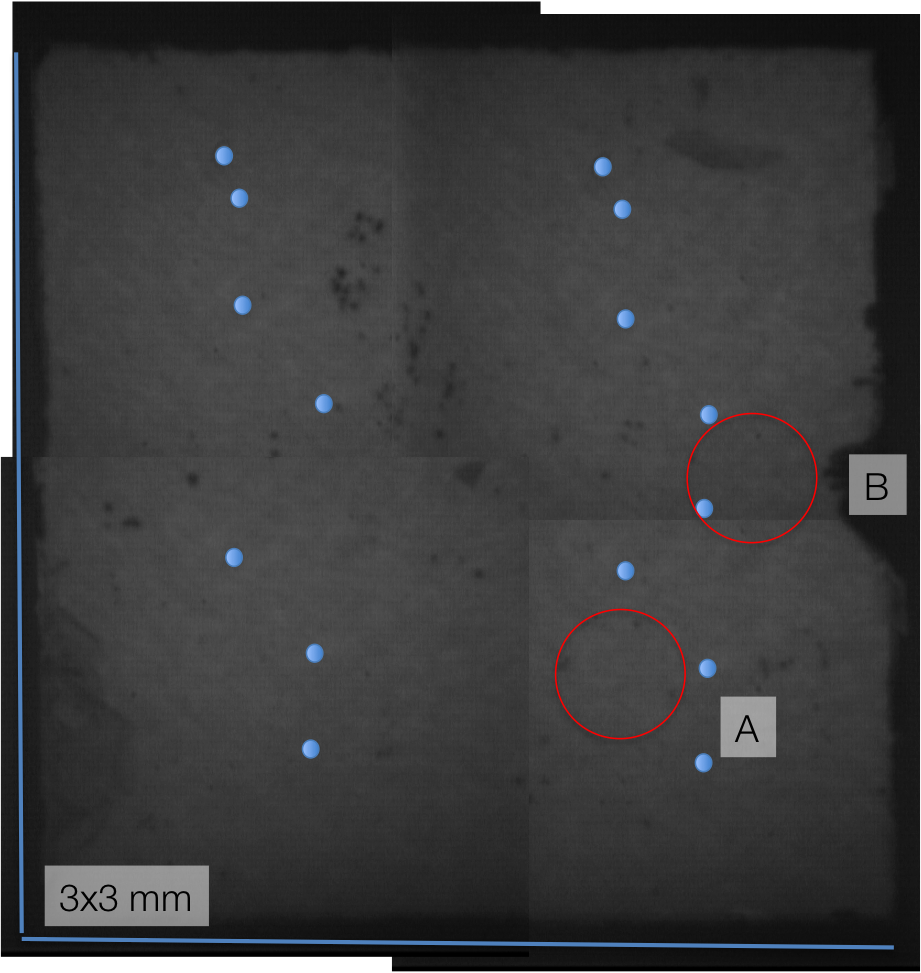
\includegraphics[width=6cm]{img/sample_surface.png}
\caption{Sample 1.
Used for pump spot scaling.
Magnified by a microscope,
illuminated with $980\,\mathrm{nm}$ light.
This light source makes visible
the defects of the structure;
as the dark spots will also be dark
when pumped during laser operation.
The blue dots cover defects
of the used camera,
which otherwise may be mistaken
as defects of the sample.
The red circles indicate
irradiation region A and B,
respectively.
The sample dimensions are $3\times3\,\mathrm{mm}$.}
\label{img:sample_surface}
\end{figure}

\begin{figure}
\centering
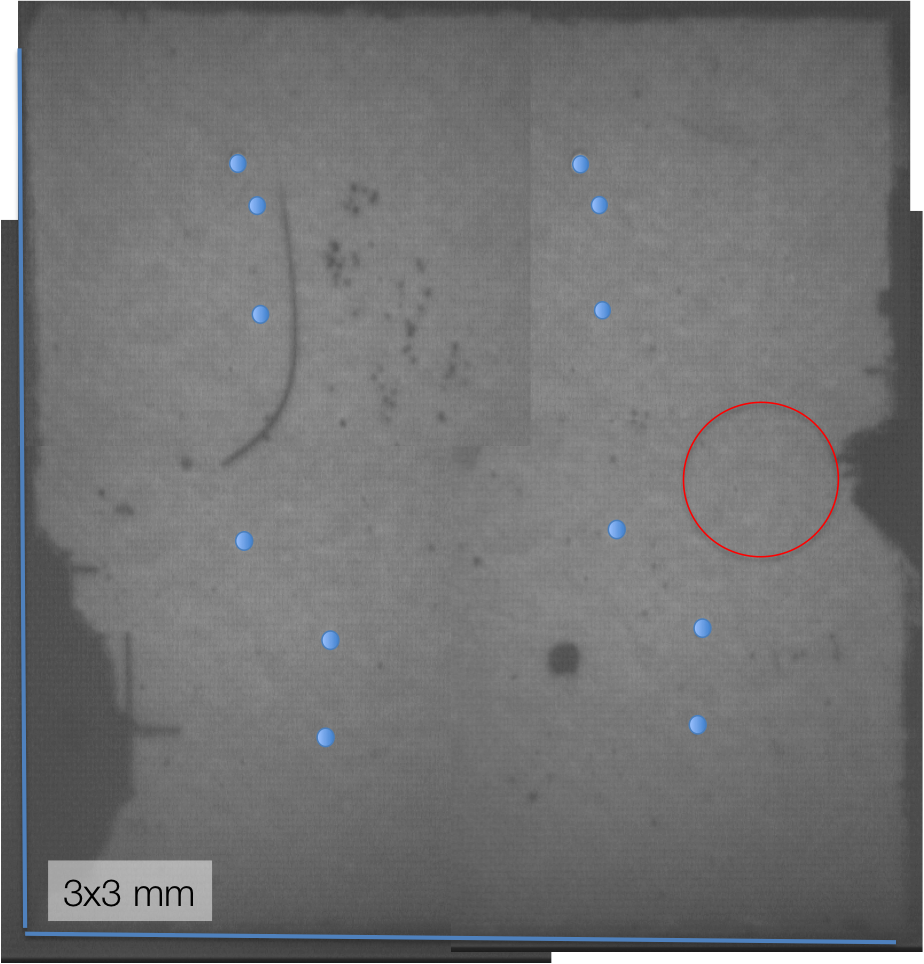
\includegraphics[width=6cm]{img/sampleAR_surface.png}
\caption{Sample 1 from Fig.~\ref{img:sample_surface},
after surface treatment and AR coating.
The brightness cannot be compared
with the one from Fig.~\ref{img:sample_surface},
the camera is not calibrated for such a comparison.
The illumination at $980\,\mathrm{nm}$
shows non-radiative defects,
but it doesn't show the surface roughness.
The red circle indicates the tested spot.}
\label{img:sampleAR_surface}
\end{figure}

\begin{figure}
\centering
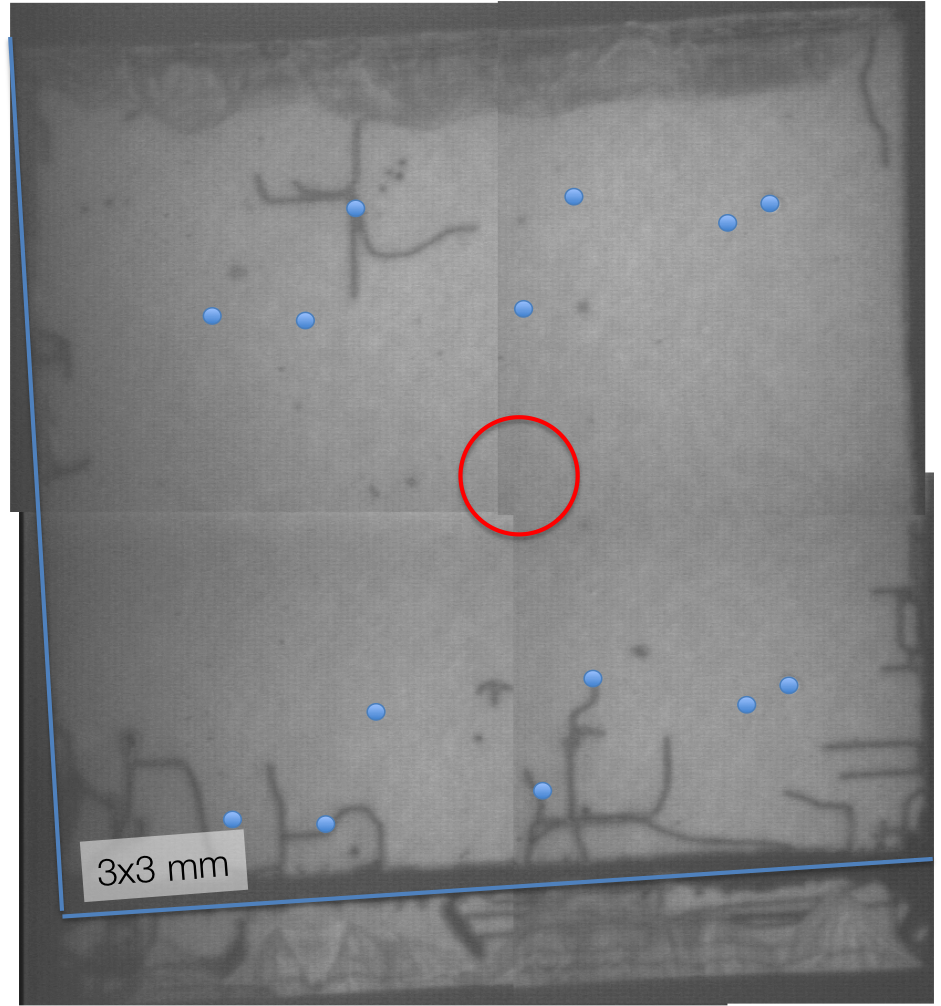
\includegraphics[width=6cm]{img/sampled6_surface.png}
\caption{Sample 2.
Used to investigate
an optimization strategy:
reflecting metalization layer behind the DBR.
The brightness cannot be compared
with the one from Fig.~\ref{img:sample_surface},
the camera is not calibrated for such a comparison.
The $980\,\mathrm{nm}$ light source
makes visible
the non radiative defects of the structure.
The blue dots cover camera defects.
The red circles indicates
the tested spot.
The sample dimensions are $3\times3\,\mathrm{mm}$.}
\label{img:sampled6_surface}
\end{figure}

\subsection{Measurement routine and error bars}
\label{sec:exp:measroutine}

For each light-light characteristic
we vary the incident pump power $P$
and the temperature of the heat sink $\Ths$.
The varying heat sink temperature
is required to determine
the thermal resistance,
see section~\ref{sec:rth}.

The heat sink temperatures are partially set
in ascending and descending order, Fig.~\ref{img:temp_order}.
This allows us to save time,
since the heat reservoir
providing the temperature stabilized water
is inert.
On the other hand,
this routine also indicates
whether the results are consistent
or depend on the temperature cycle
they were measured in.
And last but not least,
this routine allows us
to see whether or not
the sample takes damage
as a result of the elevated temperature;
a property vital for real world applications.

\begin{figure}
\centering
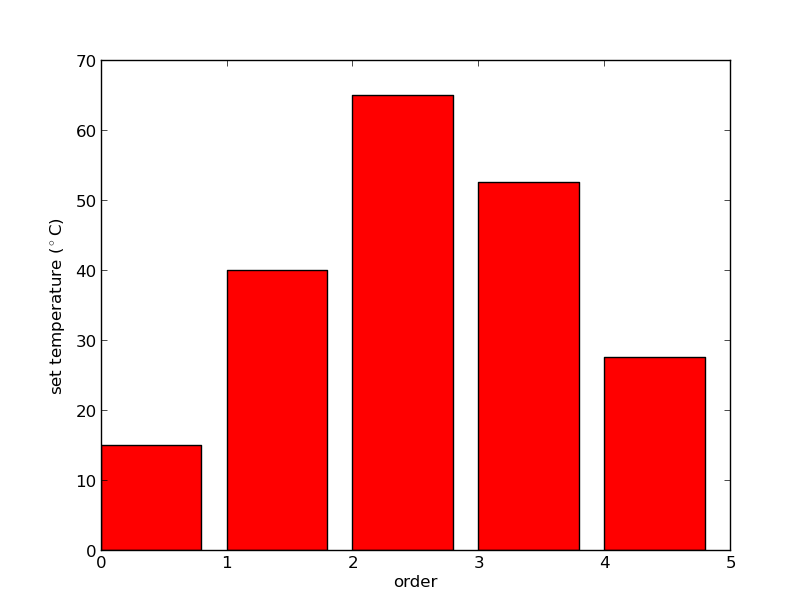
\includegraphics[width=6cm]{img/temp_order.png}
\caption{An example for the temperature order.
Some of the temperatures
are set
while heating up,
the rest while cooling down.
The objective is to save time,
to have a consistency check,
and to see whether the sample
shows fatigue after heating it up.}
\label{img:temp_order}
\end{figure}

At each heat sink temperature
we irradiate the sample
with different pump powers.
Each pump is repeated $N$ times over all.
The pump order is selected at random,
as illustrated in Fig.~\ref{img:random_sampling}.
Thanks to the random sampling
the measurement results
are detached from the lab environment --
most notably time-independent.
The heat sink cannot control its temperature
with absolute precision.
Figure~\ref{img:random_sampling_heatsink}
illustrates this issue:
It shows
the actually present heat sink temperature
for six set temperatures.
In the left column
the temperatures are plotted
in chronological order.
We can identify,
the temperature drifts.
The right column shows the same temperatures,
but corresponding to the set pump.
The repeated measurements
see a spread of different temperatures
but the temporal drifts can not be resolved.

In contrast,
Fig.~\ref{img:random_sampling_ramp_heatsink}
shows the heat sink temperature
during a measurement without the random pump selection.
In this case, clearly,
we cannot talk about a single heat sink temperature
for all the pump settings
for this specific set heat sink temperature.
The resulting measurements are highly repeatable,
but only given the same pump order.
This pseudo-stability
we exploit
during the calibration process
of the different beam samplers
and detectors:
During the calibration
we don't care about reproducibility
but solely about the repeatability
of two consecutive measurements.

\begin{figure}
\centering
\subfigure{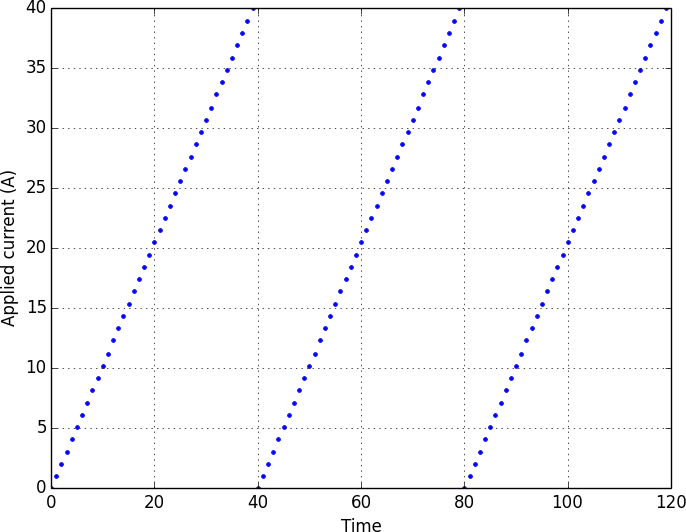
\includegraphics[width=7cm]{img/random_sampling_ramp.png}}
\subfigure{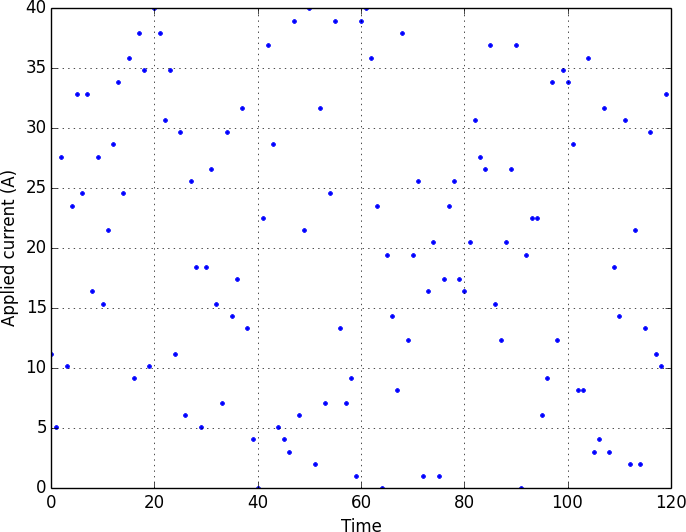
\includegraphics[width=7cm]{img/random_sampling_random.png}}
\caption{Two examples to apply various pump settings, with a repetition rate of 3.
Left: A ramp. Right: Random sampling.}
\label{img:random_sampling}
\end{figure}

\begin{figure}
\centering
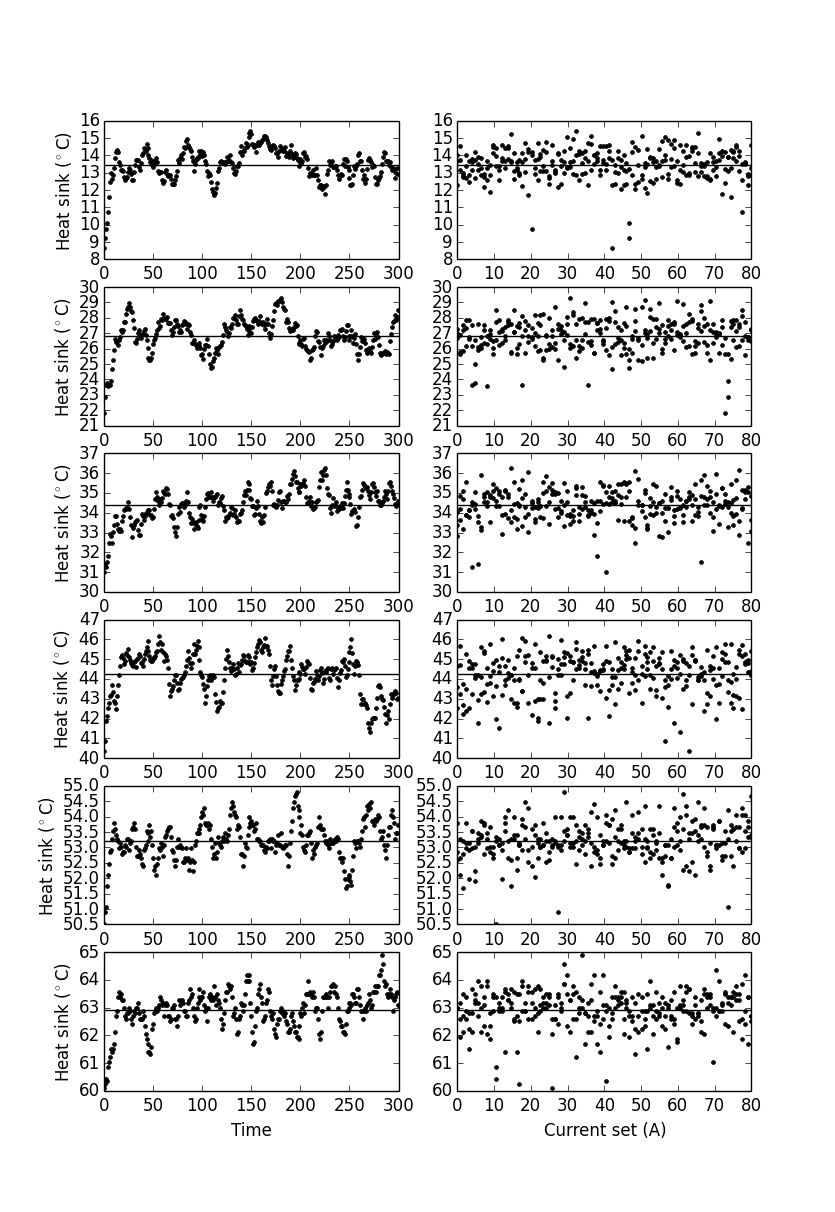
\includegraphics[width=15cm]{img/random_sampling_heatsink.png}
\caption{The heat sink temperature fluctuates over time (left).
Thanks to the random sampling addressed in Fig.~\ref{img:random_sampling}
the measurements don't see these drifts (right).}
\label{img:random_sampling_heatsink}
\end{figure}

\begin{figure}
\centering
\subfigure{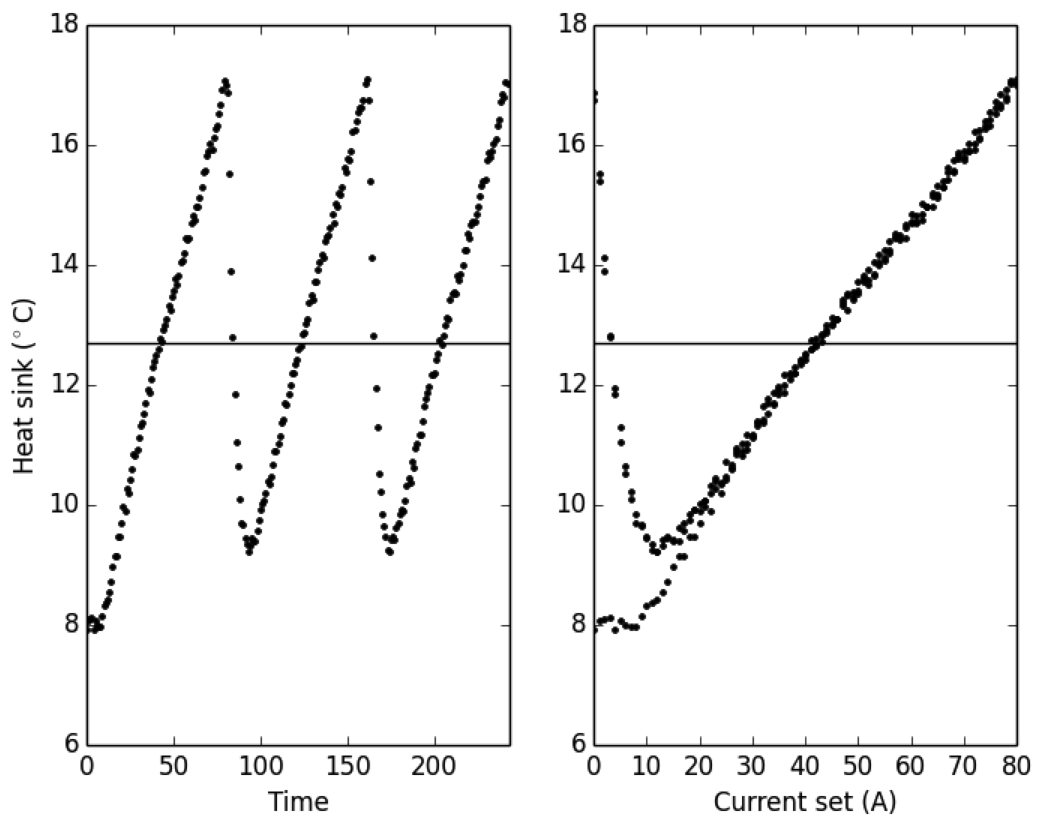
\includegraphics[width=7cm]{img/random_sampling_ramp_heatsink.png}}
\subfigure{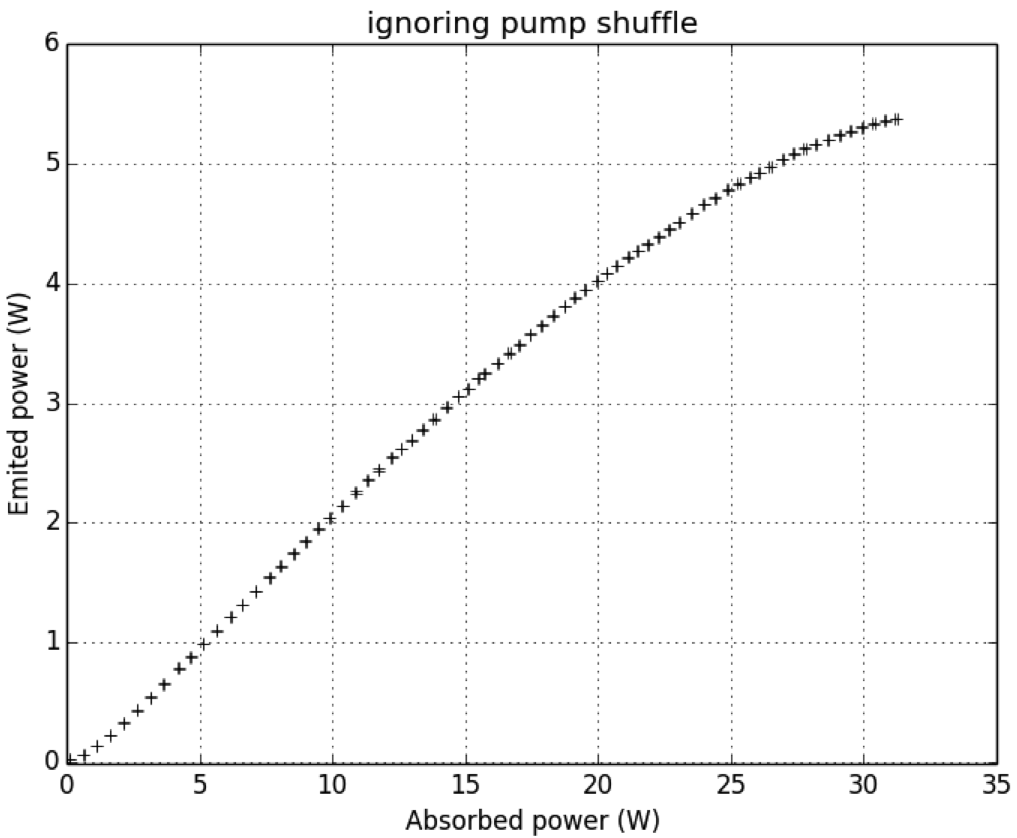
\includegraphics[width=7cm]{img/random_sampling_ramp_noisfreeLL.png}}
\caption{In contrast to Fig.~\ref{img:random_sampling_heatsink},
when we ignore the random pump sampling
highlighted in Fig.~\ref{img:random_sampling},
the temperature seen by the single pump settings
differ strongly from the average heat sink temperature
(left).
The resulting LL-characteristic
has very little noise on its data points
(right).
But these small error bars dismiss the fact
that the underlying points were measured
under very different conditions;
eroding the significance
of this low noise.}
\label{img:random_sampling_ramp_heatsink}
\end{figure}

The power meter average each measurement point
over 200 samples,
of which each one sample
takes approx. 3 ms \cite{ThorlabsPM}.

As mentioned already,
we repeated the measurement of each pump setting
$N$ times.
With this repetition we obtain a measure
for how well we know
the underlying true value.
We are hence interested in
the mean of these single measurements and
the resulting unbiased standard error \cite{Barlow}
\begin{equation}
\Delta x = \sqrt{ \frac{1}{N(N-1)}
	\sum\limits_{i=1}^N (x_i - 
		\frac{1}{N} \sum\limits_{i=1}^N x_i )^2 }.
\label{eq:sterr}
\end{equation}

For the uncertainties attached to
quantities obtained through fits,
I use a so-called
Jackknife \cite{Efron1983} approach:
In a nutshell,
this method allows to estimate
the influence of the single measurement points
on the fit parameters
without working through
the covariance matrix of the fit.
The resulting error value
is directly related with the
unbiased standard error (\ref{eq:sterr}),
used for the rest of the report.


\section{Results and Discussion}
\label{sec:eval}

In this section
I discuss
the power scaling
of our device,
the thus learned lessons
in order to improve the performance,
and an assessment of
the usefulness
of the thermal resistance
as a figure of merit
to evaluate
the samples.
I close this section
with the presentation
of an unexpected behavior
of the reflectivity
of our VECSEL device.

\subsection{Pump spot scalability}
\label{sec:eval:pumpspot}

One way to augment the output power
is to increase the pumped area
\cite{Tropper2006,Chernikov2010,Korpi2010}.
A power scalable device
would increase the output power
proportional to the irradiated area.
As described in section~\ref{sec:rth:scaling},
this ideal description
doesn't work for real VECSELs;
the lateral cooling
is important
after all
\cite{Chernikov2010}.

By investigating
the scaling behavior
we can learn about
the limits
of the performance
of our device.
We vary the pump spot size
using lenses with various focal lengths
in order to image the $200\,\mu\mathrm{m}$ diameter fiber
onto sample 1,
see section~\ref{sec:exp:setup}.
For the scaling experiments
I irradiated spot A
indicated in Fig.~\ref{img:sample_surface}.
Because of the change
of lens $\mathrm{L}_\mathrm{p2}$
and the subsequent
realignment of the setup,
I cannot ensure to have hit the exact same spot.
The employed cameras help us
to find it approximately,
but the remaining uncertainty is hard to estimate.
I imply the sample is homogeneous enough on this scale.
Each data point
is measured $N=3$ times.

\subsubsection{Output power}
\label{sec:eval:pumpspot:pwr}

In order to learn
about the scaling behavior
of the output power,
we look 
at the light-light characteristics
obtained from different
pump spot sizes.
Output scaling with area
only works up to a point,
above which
amplified spontaneous emission (ASE) losses
become significant
\cite{Hessenius2011}.
Bedford et al. \cite{Bedford2005}
also estimate
there to be
a critical diameter
above which lateral lasing
is likely to occur
before the intended
transversal lasing.
With our measurements,
we're interested
to see the experimental
scaling behavior
of our structure
for spot sizes
realistic in real world applications.

\begin{figure}
\centering
\subfigure{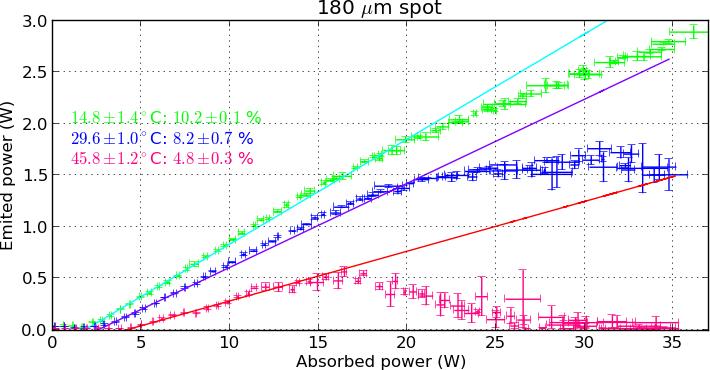
\includegraphics[width=14.5cm]{img/LL_spot180um.png}}
\subfigure{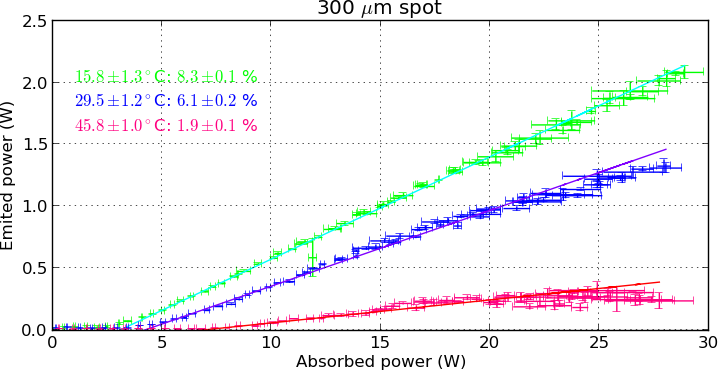
\includegraphics[width=14.5cm]{img/LL_spot300um.png}}
\subfigure{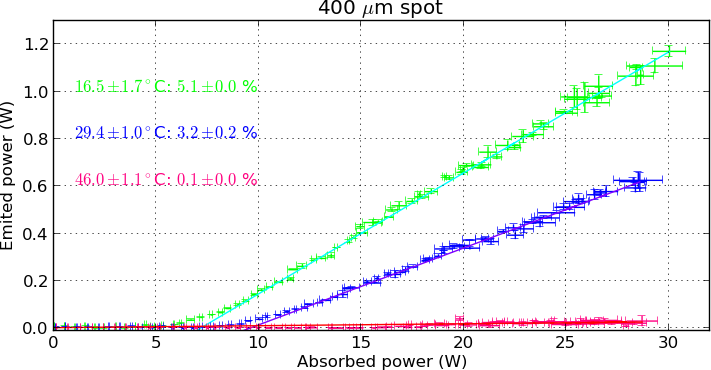
\includegraphics[width=14.5cm]{img/LL_spot400um.png}}
\caption{Light-light characteristics
for different spot sizes
obtained with spherical lenses.
The efficiency decreases
for increased spot size.
This may be due to
inefficient heat extraction
manifested in sub-area scaling of $\Rth$,
discussed in section~\ref{sec:eval:pumpspot:rth}.}
\label{img:LL_spot_scaling}
\end{figure}

Figure~\ref{img:LL_spot_scaling}
plots the resulted
light-light characteristics
for various spot sizes,
measured at the heat sink temperatures
$\{15,30,45\}\,^\circ\mathrm{C}$,
using spherical lenses
for both $\mathrm{L}_\mathrm{p1}$ and $\mathrm{L}_\mathrm{p2}$.
The average maintained heat sink temperature,
plus-minus its standard deviation,
is stated in each of the subplots,
accompanied by the slope efficiency
corresponding to
the straight lines.
The slope efficiency
is obtained
by taking into account
only the data points
of the linear segment.
The onset of
the roll over region
is ignored.

The most obvious conclusion
we can draw from these measurements
is that
our device is not power scalable:
the conversion efficiency
decreases for larger pump spots,
while in a scalable device
it should not.
Consequentially,
the maximally achieved
output power
is not increased
for larger pump spots.
In order to explain this
we acknowledge that
with larger pump spots
we're more likely
to hit non-radiative defects
\cite{Korpi2010}.
Secondly,
the thermal resistance
is empirically demonstrated
to decrease less efficiently
than with irradiated area.
The initial explanation
why VECSELs are expected
to power scale
relies on the one dimensional
heat extraction.
In reality
the contribution
of lateral cooling
must not be neglected
\cite{Chernikov2011}.

Beside the decrease
in conversion efficiency,
the roll over point
shifts to higher absorbed power
for larger pump spots.
This indicates
the structure
to heat up less
for larger pump spots.
The findings
concerning the thermal resistance
discussed in \ref{sec:eval:pumpspot:rth}
support this interpretation.

I performed
these scaling measurements
also with lens
$\mathrm{L}_\mathrm{p1}$
replaced by
an achromatic lens.
We would not assume
to find significant
differences
in the scaling behavior
since the spectral profile
of our pump source
is fairly narrow,
Fig.~\ref{img:pumpspectrum}.
Nevertheless,
this assumption needs to be tested.
Secondly,
these measurements yield
additional data points
for the thermal resistance
scaling behavior,
discussed in \ref{sec:eval:pumpspot:rth}.

The investigated spot diameters
are $\{222,333,444\}\,\mu\mathrm{m}$
for the achromatic configuration.
The used output coupler
is not optimal
for spot sizes larger than
$400\,\mu\mathrm{m}$.
The performance
corresponding to
the $444\,\mu\mathrm{m}$ spot
was indeed worse
than the one 
corresponding to
the $333\,\mu\mathrm{m}$ spot.
However,
the $222\,\mu\mathrm{m}$ spot
performed even worse.
Given this discrepancy,
I have to discard
the results
from the spot scaling experiments
in the achromatic setting.
Non the less,
all of these three measurements
showed an improved performance
with respect to
the spherical lens configuration.

We don't know the exact beam shape,
and the estimation
of the spot size
is the result
of a ray optical consideration.
The uncertainty
resulting from this approach
should be looked into more closely
in future investigations.
The fact that the pump beam shape
is relevant
was demonstrated
in \cite{Chernikov2010}.
The improved output performance
seen in our setup,
by simply changing
the type of
one of the pump delivery lenses,
also indicate
on the importance
of the pump profile.
A summary on beam shape alteration
is given
in appendix~\ref{app:spatial}
and \cite{Mansell2000}. 

For now we can only speculate
why incorporating
the achromatic lens
improves the output performance
the way it did.
I investigated
the $333\,\mu\mathrm{m}$ configuration
more thoroughly.
The results were
reproducible and thus credible.
The measurements
concerning the proposed improvements
\cite{Hader2011}
presented in section~\ref{sec:eval:maxout},
were obtained in this configuration.
\subsubsection{Thermal resistance}
\label{sec:eval:pumpspot:rth}

In order to determine the thermal resistance $\Rth$
we have to look at
the longest emitted wavelength $\lambda$
at different heat sink temperature
versus dissipated power $D$,
(\ref{eq:dissip}).
According to the method
described in section~\ref{sec:rth:lambda}
we can find a linear relation
between $\lambda$ and $D$,
from which we can deduce
the thermal resistance $\Rth$.
We do this
for the different spot sizes,
and can thus conclude
on the scaling behavior.

The spot sizes
$\{180,300,400\}\,\mu\mathrm{m}$
were each measured for the temperatures
$\{15,30,45\}\,^\circ\mathrm{C}$,
using spherical lenses
for both $\mathrm{L}_\mathrm{p1}$ and $\mathrm{L}_\mathrm{p2}$,
as described in section~\ref{sec:exp:setup}.
Figure~\ref{img:Rth_lambda_spot_scaling}
plots the resulted longest wavelengths
against dissipated power.
The average maintained heat sink temperature,
plus-minus its standard deviation,
is stated in each of the subplots.
The straight lines correspond
to the linear fit (\ref{eq:rth_fit}).
The inset text in black
takes note of this fit,
displaying the fit parameters in values.
The stated thermal resistance results from
the ratio of the two fit parameters (\ref{eq:rth_long})
\begin{equation*}
\Rth = \pd{T}{D} = \pd{\lambda}{D}/\pd{\lambda}{T}.
%\label{eq:rth_long}
\end{equation*}

In order to obtain the fit
we consider only the data points
corresponding to
the linear light-light conversion regime --
the same as for estimating
the conversion efficiency
in section~\ref{sec:eval:pumpspot:pwr},
Fig.~\ref{img:LL_spot_scaling}.
This means
we exclude both,
threshold
and roll over segments.

Figure~\ref{img:Rth_spotsizescaling}
shows the scaling of $\Rth$
with respect to spot size.
The plot to the left
displays the behavior
noted in \cite{Giet2008}
and highlighted
in section~\ref{sec:rth:scaling}:
the thermal resistance
decreases less efficiently
than by area.
The reduction in $\Rth$
is closer to $w^{-1}$
than $w^{-2}$,
as illustrated
by the slope
given in the log-log plot.

A VECSEL device is thin
compared to the pumped area.
The expected heat flow
is one dimensional,
independent on lateral cooling.
The observed scaling behavior
shows this approximation
is not tenable.
In an attempt to understand
this behavior
when we look at
the expected temperature profile
from Fig.~\ref{img:Comsol_Tvsr}.
The temperature peaks
at the center
in the case of the depicted Gauss
and super-Gaussians and,
consequentially,
lateral heat transfer occurs,
beside the one-dimensional extraction
\cite{Chernikov2011}.

The measurements conducted
with the achromatic lens
could not be used
to extract the thermal resistance
with the method described
in section~\ref{sec:rth:lambda}.
Fit (\ref{eq:rth_fit}) relies
on a linear relation
between $\lambda$ and $D$
\cite{Heinen2012}.
As will be discussed
in section~\ref{sec:eval:trollover},
Fig.~\ref{img:lambda_sample},
this linearity was not given.

The fit in turquoise
corresponds to (\ref{eq:Rth_empirical}).
With only three data points available
to fit three parameters
we cannot judge
how good the found parameters
actually are.
But given the original meaning
of $a_3$ --
an outer radius  of a VCSEL --
we recognize the found values
not to make too much sense.
The found fit is valid
only for spot sizes smaller
than $2w=550\,\mu\mathrm{m}$.
This,
together with the large uncertainties
attached to the estimates of the thermal resistance,
show there needs more work to be done
in order to get a useful statement
out of the analysis of $\Rth$.


\begin{figure}
\centering
\subfigure{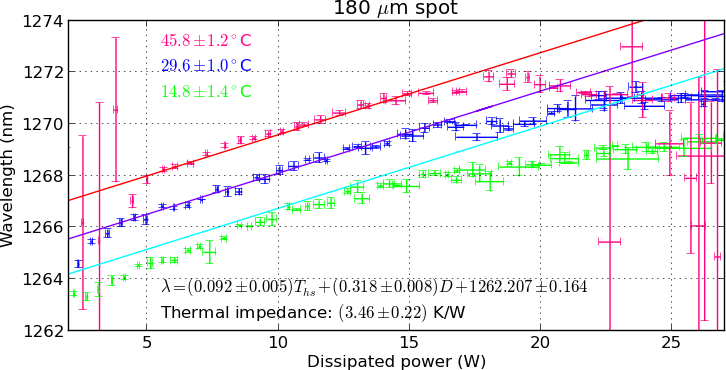
\includegraphics[width=14.5cm]{img/Rth_lambda_spot180um.png}}
\subfigure{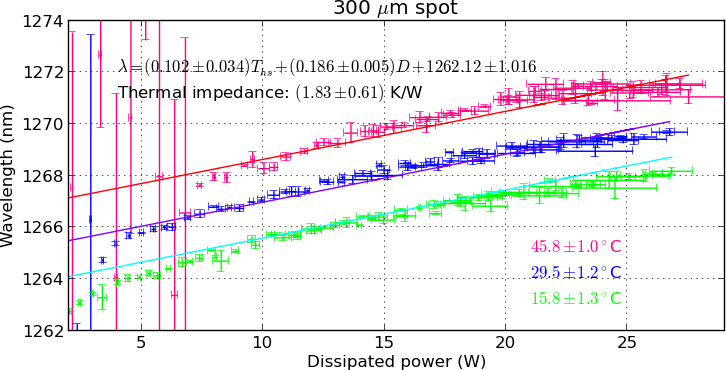
\includegraphics[width=14.5cm]{img/Rth_lambda_spot300um.png}}
\subfigure{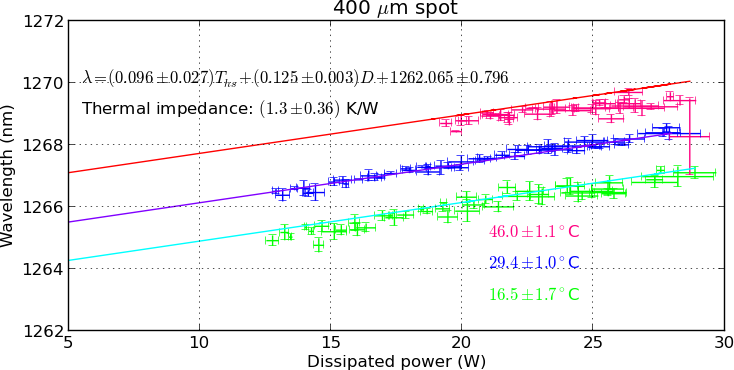
\includegraphics[width=14.5cm]{img/Rth_lambda_spot400um.png}}
\caption{Estimating $\Rth$ with
the method described in section~\ref{sec:rth:lambda}
for three pump spot sizes.
The straight lines correspond
to the fit (\ref{eq:rth_fit}),
taking into account
only the part of linear light-light conversion --
i.e. without the threshold
or roll over segments.}
\label{img:Rth_lambda_spot_scaling}
\end{figure}



\begin{figure}
\centering
\subfigure{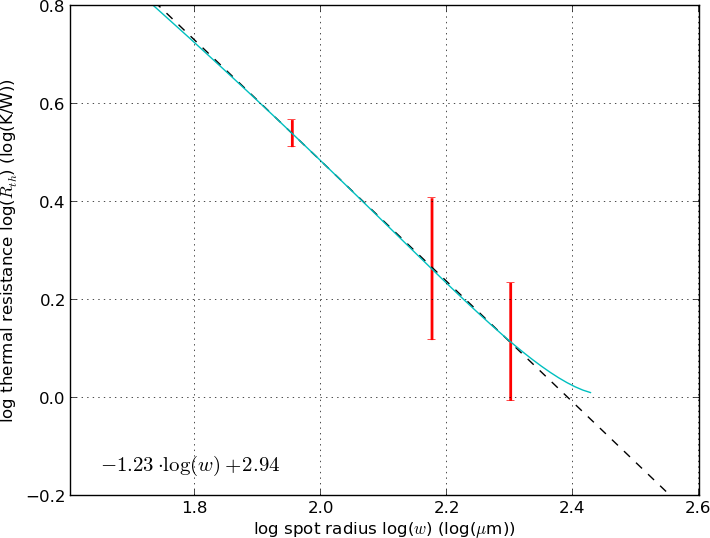
\includegraphics[width=7cm]{img/Rth_spotsizescaling_log.png}}
\subfigure{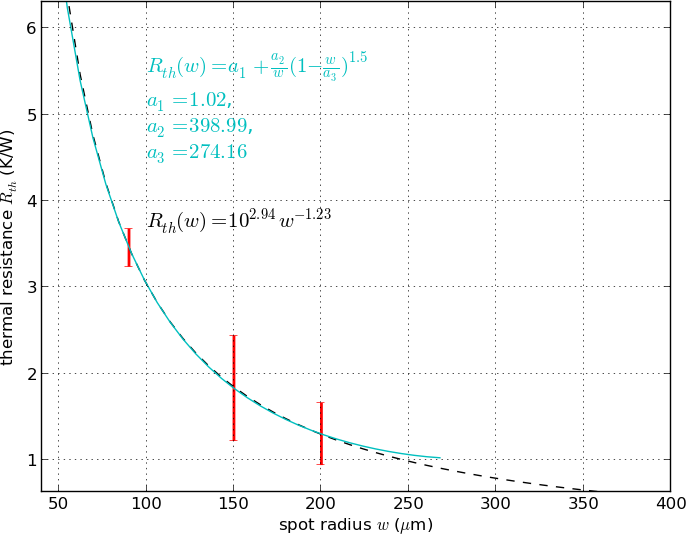
\includegraphics[width=7cm]{img/Rth_spotsizescaling_lin.png}}
\caption{Scaling of thermal resistance
(from Fig.~\ref{img:Rth_lambda_spot_scaling})
with spot size.
Its dependency on spot diameter is expected to be closer to
$(2w)^{-1}$ than $(2w)^{-2}$;
i.e. not to scale with area \cite{Giet2008}.
This is visualized by the slope in the log-log plot (left).
The continuous curve in turquoise shows a fit to
an empirical curve (\ref{eq:Rth_empirical}) \cite{Giet2008,Nakwaski1992}.
Right,
what the fits look like with linear axes.}
\label{img:Rth_spotsizescaling}
\end{figure}








\subsection{Optimized emission output}
\label{sec:eval:maxout}

Given the insights from section~\ref{sec:eval:pumpspot}
we try to optimize the emitted output further.
The following
two optimization strategies
for the VECSEL output power
are proposed
based on a microscopic many-body physics simulation
\cite{Hader2011}.
The first is to AR coat the sample:
with a $3/4$-$\lambda$ coating
appropriate for the pump wavelength
the reflection from
the air--VECSEL cap interface
(in our case InP)
should reduce
without changing the conditions
for the emission wavelength.
This intervention
permits more of the incident pump
to enter the structure,
which increases the over all
wallplug efficiency.
The second optimization is
to use a reflecting metalization layer
behind the DBR --
while leaving the DBR transparent for the pump.
This results in
the pump light
passing the active region
once more.

We investigate these two strategies
in the lens configuration
with the achromatic lens
and a $333\,\mu\mathrm{m}$
pump spot diameter.
First,
we want to record the characteristics
of sample 1 in more detail.
Once we know these,
we can apply the AR coating
on this sample
in order to compare
with its uncoated state
directly.
For the second strategy
we have to use a different sample; sample 2.
Its specifications for the active region
and DBR are identical
with the ones from sample 1.
The difference
is a different treatment
of the gold layer
contacting the diamond heat sink:
by reducing the amount of Ti
used to adhere
the DBR to the gold,
this layer shows an increase
in reflectivity.

The light-light characteristics
resulting from this more detailed analysis
is shown in Fig.~\ref{img:LL_sample}.
Each data point
is measured $N=5$ times,
as opposed to only $N=3$
for section~\ref{sec:eval:pumpspot}.
The irradiated spot is labeled B
in Fig.~\ref{img:sample_surface}.
For this spot the sample
performed best.
On the other hand,
our setup is not designed
to scan the surface in a structured manner.
The found maximum could
be only a local maximum.

\begin{figure}
\centering
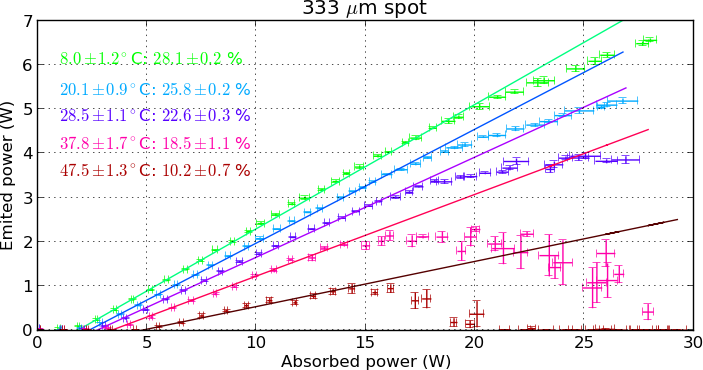
\includegraphics[width=14.5cm]{img/LL_sample.png}
\caption{Detailed LL of sample 1.
Irradiating spot B denoted in
Fig.~\ref{img:sample_surface}.
Each data point is measured $N=5$ times.
The error bars correspond
to the standard error.}
\label{img:LL_sample}
\end{figure}


\subsubsection{AR coating}
\label{sec:eval:maxout:AR}

The first optimization strategy
\cite{Hader2011}
is to apply
an anti-reflectance (AR) coating
on the sample.
In order to have
a direct comparison
we decided
to coat sample 1. 
However,
after this treatment,
the surface roughness
had visibly worsened.
In particular,
during aligning the output coupler,
in a first step we overlap
the pump spot with its reflection
from the output coupler,
using the visible aid
of a camera
along the emission path,
see appendix~\ref{app:alignment}.
Once we have found a lasing configuration
we rely on the power meter
to find the optimum alignment.

In the case of
the AR coated sample
the second spot
was hardly visible,
and looked patterned;
similar to a plastered wall.
Unsurprisingly,
the resulting light-light performance
is clearly weaker
than without the coating.
Figure~\ref{img:LL_sampleAR}
shows the resulted
light-light conversion.

Based on the stated observations,
we cannot compare
the two measurements.
We have to improve the coating process
before we can evaluate this optimization strategy.

\begin{figure}
\centering
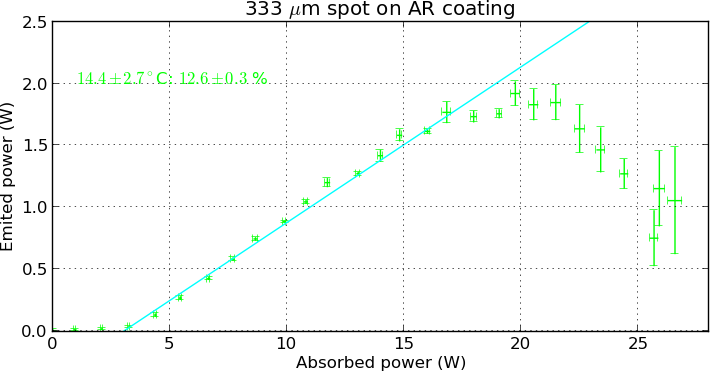
\includegraphics[width=14.5cm]{img/LL_sampleAR.png}
\caption{The AR coating
applied on sample 1 worsened its performance.
Given the observations made
during measurements
(see text),
this is a verdict most likely
not tenable for AR coating in general,
but concerns the quality of our coating in particular.}
\label{img:LL_sampleAR}
\end{figure}

\subsubsection{Reflecting metalization layer: record output}

For the second optimization strategy
\cite{Hader2011}
we use a sample
whose metalization interface
between DBR and CVD diamond
was treated to be highly reflective.
Sample 2 is measured
irradiating the spot
indicated with a red circle
in Fig.~\ref{img:sampled6_surface}.
The light-light characteristic
is depicted in Fig.~\ref{img:LL_sampled6}.

Apparently,
a lot more of the absorbed light
is converted into laser output
(nearly $60\,\%$
at \degr{5} heat sink temperature).
On the other hand,
the over all reflectivity off the sample
is higher for sample 2
than for sample 1.
This fact I revisit
in section~\ref{sec:eval:refl}. 

Table~\ref{tab:LL_sampled6} highlights
the observed peak performances.
These, coincidentally,
represent the new
(unofficial)
world record
in emitted power
in the $1300\,\mathrm{nm}$ waveband.
The highest reported emission power
for this waveband so far
was $7.1\,\mathrm{W}$
in a intracavity heat spreader configuration
using a pump spot diameter of $300\,\mu\mathrm{m}$
at a heat sink temperature
of \degr{7}
\cite{Sirbu2014OptExp}.

Figure~\ref{img:conversion_temp}
shows a comparison between
sample 1 (uncoated)
and sample 2.
The latter appears to be
about twice as efficient
in converting the absorbed light.
However,
this cannot directly be attributed
to the second pass
through the active region
with this optimized design.
In sample 1
we don't distinguish
whether the pump is absorbed
in the active or the metalization layer.
Our definition of absorbed power,
$A=P-R$ (\ref{eq:abspwr}),
looks only at the difference
of power in the pump
and the reflection channel.
The contribution
from the reflected power
is indeed larger
for sample 2,
discussed in section~\ref{sec:eval:refl}.

\begin{figure}
\centering
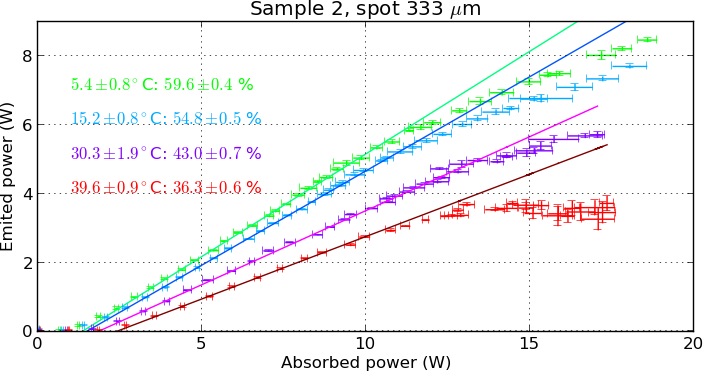
\includegraphics[width=14.5cm]{img/LL_sampled6.png}
\caption{Light light performance
of sample 2,
with the gold interface
between DBR and CVD diamond
treated to be highly reflective.
The irradiated spot
is indicated
in Fig.~\ref{img:sampled6_surface}.
Each data point
represents an average
over 5 repetitions.}
\label{img:LL_sampled6}
\end{figure}

\begin{table}[h]
\centering
\caption{Highlighting the peak data from Fig.~\ref{img:LL_sampled6}.
The error values correspond:
to the standard deviation for the heat sink,
and to the standard error (\ref{eq:sterr})
for the absorbed and emitted power.
Pump spot diameter is estimated
as $333\,\mu\mathrm{m}$.
The incidence angle
is $\approx36^\circ$.}
\begin{tabular}{rrr}
\hline
Heat sink (\degr{}) &
absorbed power ($\mathrm{W}$) & emitted power ($\mathrm{W}$) \\
\hline
$5.4\pm0.8$ & $18.6\pm0.3$ & $8.46\pm0.06$ \\
$15.2\pm0.8$ & $18.1\pm0.5$ & $7.7\pm0.06$ \\
$30.3\pm1.9$ & $17.1\pm0.2$ & $5.72\pm0.09$ \\
$39.6\pm0.9$ & $17.4\pm0.2$ & $3.7\pm0.2$ \\
\hline
\end{tabular}
\label{tab:LL_sampled6}
\end{table}

\begin{figure}
\centering
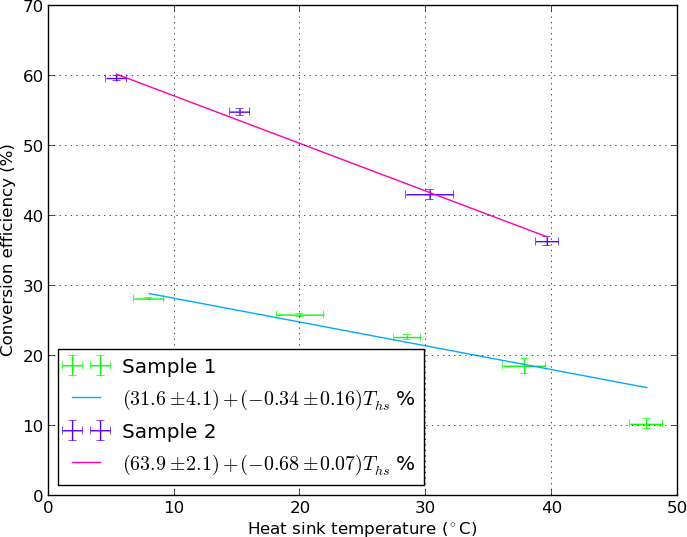
\includegraphics[width=14.5cm]{img/conversion_temp.png}
\caption{Summary of the values found in
Fig.~\ref{img:LL_sample} and \ref{img:LL_sampled6}.
The conversion efficiency of sample 2
corresponds to approximately twice
the value of sample 1.
The ultimate limit of conversion efficiency
is given by the quantum defect
$\lambda_\mathrm{pump}/\lambda_\mathrm{laser}=77.5\,\%.$}
\label{img:conversion_temp}
\end{figure}
\subsection{Intrinsic roll over temperature}
\label{sec:eval:trollover}

One method to estimate the thermal resistance
looks at the dissipated power at roll over,
linked with the heat sink temperature --
see section~\ref{sec:rth:trollover}.
This method relies on an intrinsic roll over temperature,
independent of the heat sink temperature:
we associate
the longest emitted wavelength
with a temperature
in the active region.
If roll over occurs
because the active
exceeds a critical temperature,
the emitted wavelength
at this point
should be the same
regardless of the heat sink temperature
\begin{equation}
T_\mathrm{ro} = \Ths + \Rth D_\mathrm{ro}.
\end{equation}

We don't know
whether all VECSEL structures
show this behavior,
or whether it depends on the device.
It is thus necessary
to first test the hypothesis
by looking at the spectrum
emitted at roll over.
Once this is established
the method described
in section~\ref{sec:rth:trollover}
is more convenient
for estimating $\Rth$.

Our measurements
were pump limited.
Not every investigated 
spot size and heat sink temperature
did reach roll over.
This would be necessary
in order to extract
the thermal resistance
with said method.
However,
I can highlight
the emitted spectra
of those settings that did reach roll over.

The pump spot size scaling measurements
of sample 1
depicted in Fig.~\ref{img:Rth_lambda_spot_scaling}
suggest an ultimately
longest emitted wavelength
of about $1271\,\mathrm{nm}$.
In the case of the $180\,\mu\mathrm{m}$
the measurements corresponding to
a heat sink temperature of
\degr{30} and \degr{45}
both even out at this wavelength.

In the configuration
with lens $\mathrm{L}_\mathrm{p1}$
being achromatic
the observed spectrum behaves differently.
Figure~\ref{img:lambda_sample}
shows this exemplary
for the spectra
corresponding to
the measurements presented
in Fig.~\ref{img:LL_sample}.
The longest emitted wavelength
does not depend linearly
on dissipated power.

Consequentially,
I cannot apply the linear regression
suggested in \ref{sec:rth:lambda},
\cite{Heinen2012},
in order to extract $\Rth$.
In principle,
I could evaluate the derivatives
$\frac{\partial \lambda}{\partial D}$
and $\frac{\partial \lambda}{\partial T}$
numerically.
However,
due to the fluctuations on $D$
it is not clear
how to evaluate
$\frac{\partial \lambda}{\partial T}$
in practice.
I therefore withstand
to call out a number for $\Rth$
based on the presented results.

Concerning longest emitted wavelength,
in Fig.~\ref{img:lambda_sample}
we see the measurements
corresponding to
$\Ths=\{48,38,29\}\,^\circ\mathrm{C}$
to converge to the same value.
This limit wavelength is,
however,
longer than suggested
by Fig.~\ref{img:Rth_lambda_spot_scaling}.
The spectrum of sample 2,
plotted in Fig.~\ref{img:lambda_sampled6},
does not allow to infer
on the behavior of the peak wavelength.

In conclusion,
the available data
on emitted longest wavelength
do not give a clear picture
whether $\lambda_\mathrm{ro}$
is independent of the heat sink temperature
or not.
On the other hand,
even if the assumption
of an intrinsic roll over temperature
is valid,
there is another problem
with the method presented in \ref{sec:rth:trollover}:
it is supposed to be less error-prone,
as mode fluctuations
between two measurements
are expected to yield
a considerably large uncertainty
in $\lambda$ \cite{Heinen2012}.
As shown in section~\ref{sec:eval:pumpspot:rth}
the obtained values for $\Rth$,
using the spectra dependent method \ref{sec:rth:lambda},
indeed do have a large uncertainty attached.
But this comes not from the uncertainty
of the single data points.
The error bars along $\lambda$ are small
compared to the fluctuations
in estimated dissipated power.

Ultimately,
the uncertainties
attached to the extracted thermal resistance
come from the assumption  
$\frac{\partial \lambda}{\partial D}$
and $\frac{\partial \lambda}{\partial T}$
to be linear.
Likewise,
at least in our setup,
the exact point of roll over
is difficult to estimate.
Therefore,
deducing $\Rth$
using the roll over point
does not result in a more accurate value.


\begin{figure}
\centering
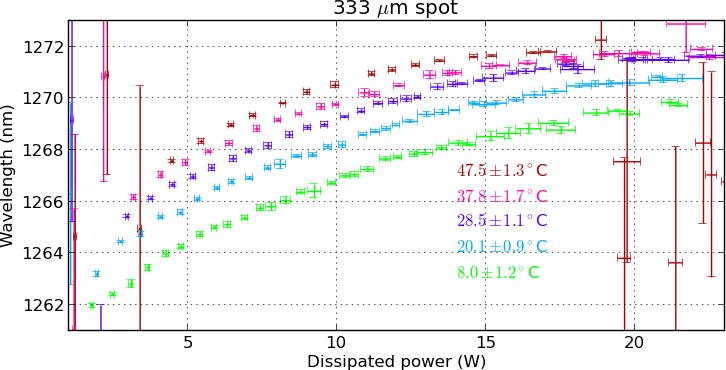
\includegraphics[width=14.5cm]{img/lambda_sample.png}
\caption{Longest emitted wavelength
recorded in the achromatic lens configuration
of sample 1.
The observed non-linear relation was not expected
given the discussion in section~\ref{sec:rth:lambda}.
The longest emitted wavelength
over all
seem to converge to a heat sink independent value.
This is in line with
the hypothesis of an intrinsic roll over temperature
suggested in section~\ref{sec:rth:trollover}.}
\label{img:lambda_sample}
\end{figure}

\begin{figure}
\centering
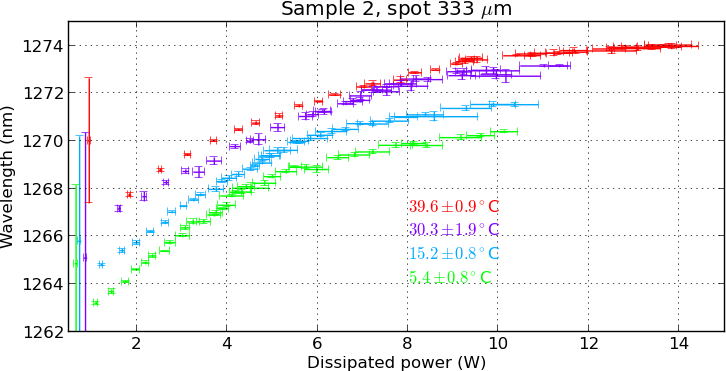
\includegraphics[width=14.5cm]{img/lambda_sampled6.png}
\caption{Longest emitted wavelength
recorded in the achromatic lens configuration
of sample 2.
The over all longest emitted wavelengths
appear not to converge
to the same value
for each of the heat sink temperatures.}
\label{img:lambda_sampled6}
\end{figure}
\subsection{Pump-induced change in reflectivity}
\label{sec:eval:refl}

We monitor the reflectivity
of the sample during the measurements.
The amount of reflected light
is an important quantity
to estimate the dissipated power $D$ (\ref{eq:dissip}),
which itself is important
in order to asses the heat flow
in the VECSEL device \cite{Heinen2012}.
It turns out,
the reflected fraction
is not constant.
Instead,
it depends on
the incident pump power
and the heat sink temperature.

This observation of reflectivity
was so far not reported
in literature.
In this section
I present the general observations,
followed by a more detailed
analysis of the reflectivity
in the low pump regime --
what I will call base reflectivity.
The section closes
presenting some potential effects
that may contribute
to this phenomenon.

\subsubsection{Observation}

The reflectivity
off the VECSEL structure,
$r=R/P$,
changes depending on
the heat sink temperature
and the pump power.
Figure~\ref{img:basereflectivity}
illustrates this statement.

\begin{figure}
\centering
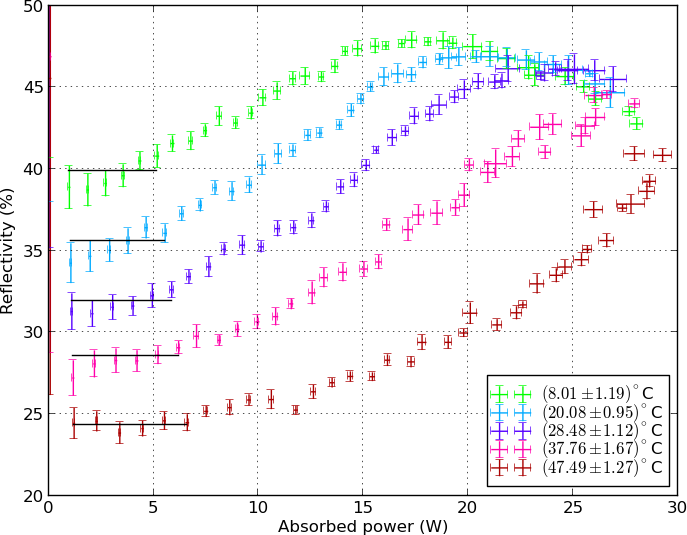
\includegraphics[width=14.5cm]{img/basereflectivity_temperatures.png}
\caption{Sample 1.
The reflectivity
changes depending on pump power
and heat sink temperature.}
\label{img:basereflectivity}
\end{figure}

On the one hand side,
the reflectivity decreases
for an increase
in heat sink temperature.
With higher absorbed power
the temperature
inside the device
increases further.
However,
for higher absorbed power
the reflectivity increases.
Consequentially,
the pump induced change in reflectivity
cannot be a purely thermal effect.

The lasing activity
of the device
potentially affects the reflectivity.
In order to test for this,
I measured
the reflected light
when we remove the output coupler.
Figure~\ref{img:basereflectivity_nooc}
plots three temperatures
measured with
(depicted in Fig.~\ref{img:basereflectivity})
and without the output coupler.

\begin{figure}
\centering
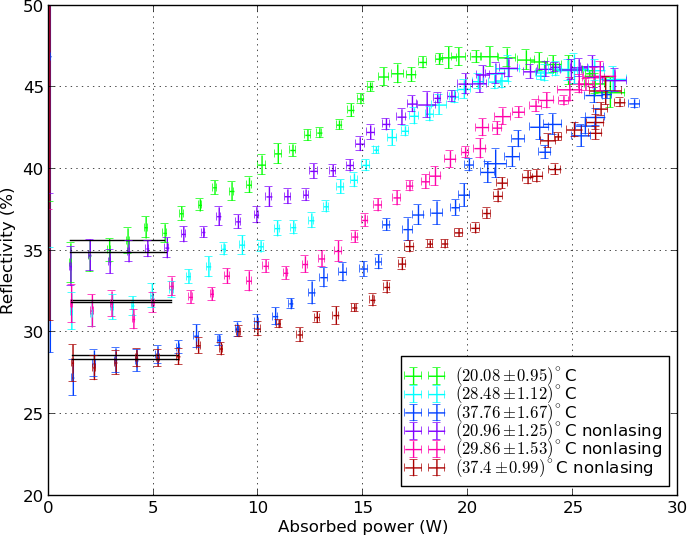
\includegraphics[width=14.5cm]{img/basereflectivity_noOC.png}
\caption{Sample 1.
Reflectivity without output coupler.}
\label{img:basereflectivity_nooc}
\end{figure}

The low pump regime reflectivity
(base reflectivity)
is unaffected
by the presence or absence
of the output coupler.
Increased pump
leads to an increase
in reflectivity;
qualitatively similar
to the lasing configuration.
But,
quantitatively,
this increase is less steep
when we remove the output coupler.

Once the reflectivity has reached
its peak value
it decreases again.
The point of peak reflectivity
does not coincide
with an apparent effect
in the light light performance,
Fig.~\ref{img:LL_sample}.

We have treated sample 1
with an anti-reflectance coating,
in an attempt to investigate
an optimization strategy,
laid out in section~\ref{sec:eval:maxout:AR}.
Figure~\ref{img:refl_sampleAR}
demonstrates the base reflectivity
indeed to be lowered.
The AR coated device
also shows an increase
in reflectivity
for higher pump.


\begin{figure}
\centering
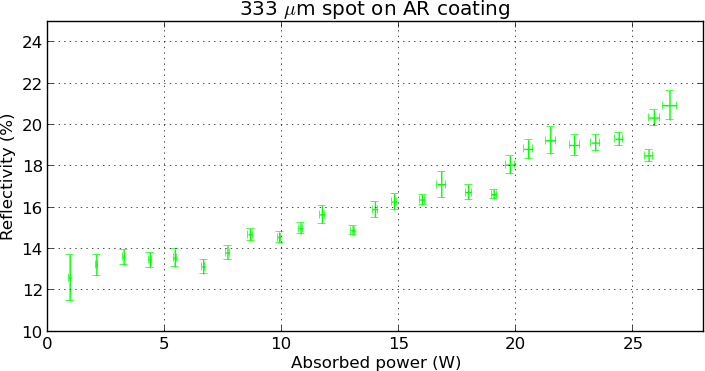
\includegraphics[width=14.5cm]{img/refl_sampleAR.png}
\caption{Sample 1 AR coated.
While the AR coating wasn't successful
to improve the light-light performance,
the base reflectivity indeed was reduced.
The heat sink temperature was
$14.4\pm2.7\,^\circ\mathrm{C}$.
The uncoated sample showed
a base reflectivity of about $38\,\%$
for this temperature.
The coating hence successfully
lowered the reflectivity
to about a third.}
\label{img:refl_sampleAR}
\end{figure}

In Fig.~\ref{img:basereflectivity}--\ref{img:basereflectivity_d6}
the relative reflectivity,
$r=R/P$,
is plotted
against absorbed power $A=P-R$.
A priori
it is not clear
whether this is a good choice.
However,
by doing so
the reflectivity curves
of the different heat sink temperatures
overlap in the decrease regime
after the peak reflectivity.
This overlap
is present for both samples,
and even more apparent
in Fig.~\ref{img:basereflectivity_d6}
of sample 2.
Maybe,
this hints at
an intrinsic limit
of the VECSEL structure.
Plotting $P$ for the x-axis,
the declining line
of the different heat sink temperatures
are shifted with respect to each other.
With $D$ for the x-axis,
the data points corresponding
to the lasing configurations
in Fig.~\ref{img:basereflectivity_nooc}
are shifted left,
such that those
without the output coupler
overshoot the stated line
of decreasing reflectivity.


\subsubsection{Base reflectivity}

For low pump power
the relative reflectivity
shows a flat plateau.
The weighted mean reflectivity
of the regime between 1--$9\,\mathrm{W}$
of pumped power
I call base reflectivity
(the $9\,\mathrm{W}$ is an arbitrary cut,
based on Fig.~\ref{img:basereflectivity}).
This base reflectivity
follows a linear relation
as a function of heat sink temperature.
This is plotted in
Fig.~\ref{img:basereflectivity_fit}
and \ref{img:basereflectivity_d6}
for sample 1 and 2,
respectively.

Sample 2 seems to be about $50\,\%$
more reflective
than sample 1.
Qualitatively,
the increase in reflectance
can be expected.
By reducing the amount
of Ti used
to connect DBR with Au,
the amount of reflected pump light
from this interface
increases \cite{Hader2011}.
This is exactly the difference
between sample 1 and 2,
see section~\ref{sec:basics}.

\begin{figure}
\centering
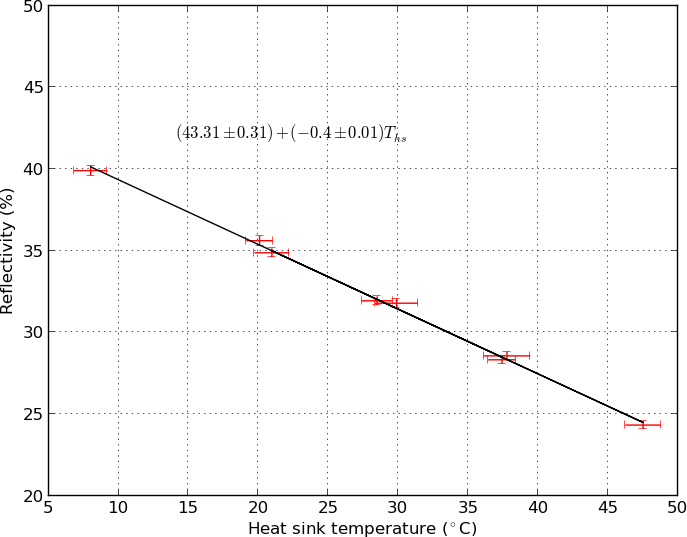
\includegraphics[width=14.5cm]{img/basereflectivity_fit.png}
\caption{Sample 1.
The base reflectivity follows a linear relation
with the heat sink temperature.
The presence of the output coupler
does not affect this low pump regime.
The corresponding measurements
are therefore included.
See Fig.~\ref{img:basereflectivity}
and \ref{img:basereflectivity_nooc}.}
\label{img:basereflectivity_fit}
\end{figure}

\begin{figure}
\centering
\subfigure{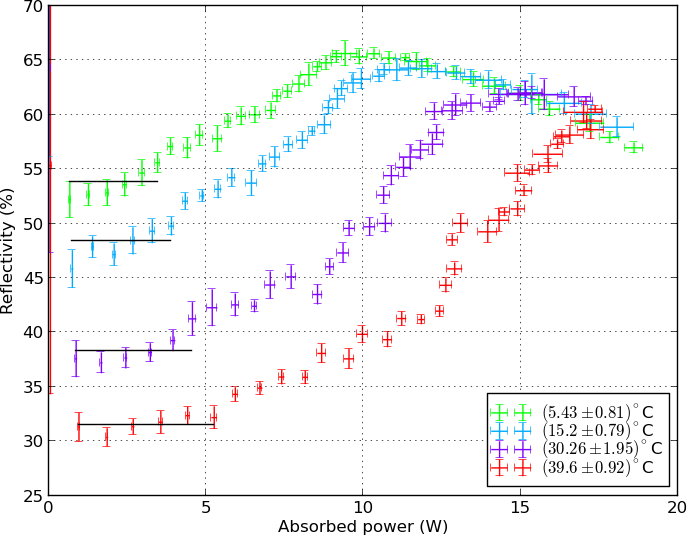
\includegraphics[width=7cm]{img/basereflectivity_temperatures_d6.png}}
\subfigure{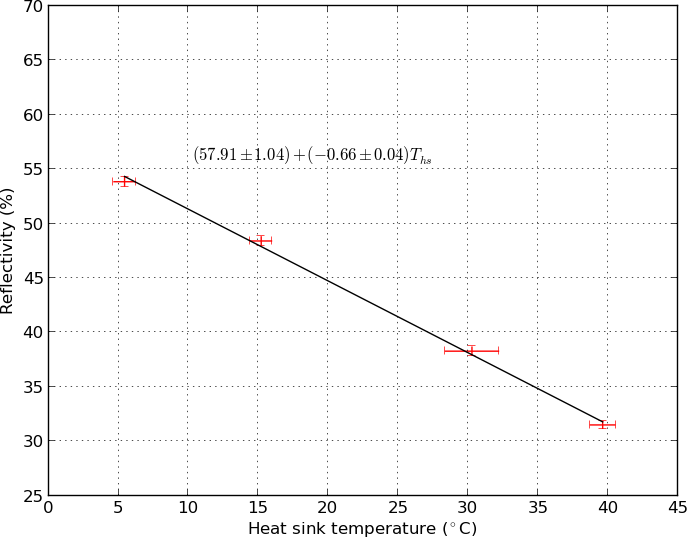
\includegraphics[width=7cm]{img/basereflectivity_d6_fit.png}}
\caption{Sample 2.
The reflectivity
is higher than that for sample 1.
In sample 2 the gold layer
connecting the DBR with diamond
is reflective
while for sample 1,
it absorbs the residual pump.
Compared to Fig.~\ref{img:basereflectivity_fit}
sample 2 is about $50\,\%$
more reflective than sample 1.}
\label{img:basereflectivity_d6}
\end{figure}


\subsubsection{Explanation candidates}

The low pump regime
should be governed
by the simple reflectivity
due to the multi layer nature
of our device.
In order to calculate
this reflectivity value
we need to know
the refractive indices
and absorption coefficients
of all the used AlInGaAs compounds
in our structure.
We don't have access
to such a complete table,
so I cannot calculate this numeric limit. 

Literature
does not provide
a satisfying answer
for this pump induced reflectivity change.
The effect of thermoreflectance
appears to be a related candidate.
It is used for temperature measurements
based on the change in surface reflectivity
\cite{Epperlein1993,Pierscinski2009}.
Accordingly,
the incident pump
perturbes the thermal equilibrium
of the probed structure.
The reflectivity then changes
as a result of this induced modulation.
In semiconductors,
the relationship
between the variation in
optical reflectivity
and temperature
is mainly due to the temperature dependence
of the band gap \cite{Tessier2001},
\begin{equation}
\Delta R = \dd{R}{T} \Delta T.
\end{equation}

The thermoreflectance coefficient $\dd{R}{T}$
varies strongly
with the probed material
and the probe wavelength.
It cannot reliably be simulated numerically,
but has to be determined experimentally
\cite{Pierscinski2009}.
This procedure is time
and equipment intensive.
For this report I omit
determining the thermoreflectance coefficient
of the sample at hand.
Consequentially,
I cannot fit the expected thermoreflectance curve
onto the measured behavior.
And I cannot conclude
whether this concept
leads into the right direction.

The thermal change
in refractive index
is unlikely to be
a relevant contributor
to the pump induced
change in reflectivity:
it depends only weakly on temperature,
$\frac{1}{n_\mathrm{InP}}\frac{\d n_\mathrm{InP}}{\d T}=
2.7(3)\times10^{-5}\,\mathrm{K}^{-1}$
\cite{SpringerMat}.
This change is relevant
for the shift in emission wavelength
and hence section~\ref{sec:rth:lambda}.
But reflectivity
changes in the order of
$R=|\frac{n-1}{n+1}|^2$,
where temperature induced change in $n$
is unlikely to be relevant.

On the other hand,
the barriers are designed to absorb
the incident pump light.
Consequentially,
the temperature dependent band gap change
is of large relevance.

Given the observation
that the change in reflectivity
is not solely a thermal
effect,
we have to assume
there are
(at least)
two different mechanisms
at work.
Motivated by the thermoreflectance,
first,
we attribute
the decrease in base reflectivity
to the band gap of the semiconductor:
As a result of
the elevated temperature
the quantum wells
show a more metallic nature.
Such a structure can absorb
the incident pump
with higher efficacy,
which leaves
less power in the reflection channel.

A second contributing effect
is due to the creation
of electron hole pairs.
By increasing the pump power,
the electron hole pair creation depletes.
At this point
more of the incident light
is not absorbed
and can be reflected
from one of the many layers.

The AR coated sample
showed a decrease
in base reflectivity,
while the uprise
for higher pump power
persisted.
This indicates
the base reflectivity
to be a result
of the many layer structure,
while the reflectivity increase
is due to an internal change.

If the laser emission
is solely relevant
as a cooling channel,
the curves with and without output coupler
should overlap,
when plotted against dissipated power.
However,
with dissipated power,
$D=A-E$,
the data points
from the output coupler configuration
would shift left,
which increases the difference between
the two curves
even more.

Instead,
the explanation
of electron hole pair depletion
expects the reflectivity
to increase faster
in the scenario
the electron hole pairs
are created
due to the stimulated interaction
with the cavity.
In absence of the output coupler
these pairs are still created
because of thermal excitation,
but at a lower rate.
This is what we can see
in Fig.~\ref{img:basereflectivity_nooc}.

Whether my simplistic argument
concerning the bandgap
and electron hole excitation
is tenable,
I leave open
for someone else to discuss.
One objection for example
is that we don't see
an excitation saturation
in the emission measurements.
Secondly,
this explanation
is held very generally
so that
the observed effect
should  appear also in other
VECSEL structures.
I cannot find a publication
describing our observations.




\section{Conclusion}
\label{sec:conclusion}

I have presented
the power scaling behavior
of our wafer-fused
$1300\,\mathrm{nm}$ waveband
VECSEL device
in the thin disk (flip-chip)
heat dissipation scheme.
This scaling was found
to be below
the expected behavior
for disk lasers,
but are in line with
other published findings.
It is assumed
to be a result
of the sub-area scaling
of the thermal resistance --
whose scaling behavior
was also demonstrated
in this report.

Changing the pump configuration
to incorporate an achromatic lens,
resulted in significantly
improved output performance.
In this configuration
I have investigated
upon two optimization strategies:
(i) anti-reflectance (AR) coating,
(ii) improved reflectivity
of the Au bonding layer
between DBR and heat sink.
This second strategy
resulted in record output power
of $8.5\,\mathrm{W}$
for a heat sink temperature
of \degr{5}.
The AR approach we had to
abandon due to insufficient
coating quality.
The found difference
in output performance
as a result of
changed pump conditions
suggests the pump beam profile
to be more important
than usually assumed.
As such,
a carefully prepared pump
is likely to improve
a VECSEL's performance,
while keeping the chip design.

The longest emitted wavelength,
resulting from the heating
of the VECSEL device
due to increased pump power,
appears to tend to a value
that is independent of
the applied heat sink temperature.
This finding suggests
the power roll over
of our device
to occur at
an intrinsic critical temperature;
this property
was thus far not confirmed
for our structure.
It allows
to determine
the thermal resistance
in a way
that doesn't rely
on a spectral shift
of the emitted light.

Furthermore,
I have presented
the reflectivity
off our VECSEL structure
to change
for higher pump power.
This behavior
has so far not been reported.
By taking into account
these measured reflectivity values --
instead of assuming
the reflectivity
to remain at its low pump reflectivity level --
also the found conversion efficiency
of our device
showed record results;
up to nearly $60\,\%$ for
\degr{5} heat sink temperature.

Beside these direct results,
I have assessed
two methods
to experimentally
determine the thermal resistance
of a VECSEL,
that can be measured
simultaneously with
regular light-light characteristics.
I have to conclude
these methods
not to yield
a good figure of merit.
The identified dependencies
inevitably link
the resulting thermal resistance
with the setup it was measured with.
I have showed these shortcomings
by means of
experiment --
the spectral behavior
varied as a result
of the pump conditions --
and numerical considerations.

The presented
maximum output power
reached during this project is
limited by pump power,
heat sink temperature stability,
and the lack of control
over the pump conditions --
most notably
the pump distribution.
In addition,
the investigated samples
show a high reflectivity,
such that a considerable amount
of pump is wasted.
For future works
I suggest to invest
time and resources
directed at these domains.
The sample reflectivity
could also be exploited
by using a mirror arrangement
that recycles
the reflected power
and redirects it
onto the pumped spot.

This report acts
as basis
to reach out
to other groups,
who have already
heavily invested
in numerical approaches:
if the improvements in output performance
indeed can be partially attributed
to the change in pump profile,
more effort
should be put into investigating
this aspect
for VECSEL applications.
One of the key arguments
of VECSELs
is their capability
to convert low-cost pump light
into high quality laser emission.
If this conversion
can be improved
by simple modifications
in the pump channel,
such findings
may benefit
a large variety of VECSEL applications.
Additionally,
it will be interesting
to see the detailed reflectivity behavior
of other devices.

As a last point,
the presented measurements
have demonstrated
the high degree
of sample integrity:
our wafer-fused devices
did not show
any signs
of degradation.
And this despite the fact
that the samples were heated up
and cooled down
over a broad range of temperatures;
the samples were exposed to
beyond roll over pump powers;
the pump irradiation
did not occur
in a smooth ramp order
but were randomly sampled
instead.
These findings
demonstrate a high device quality,
obtainable by wafer fusion.


\newpage
\appendix
\section{Alignment process, description of}
\label{app:alignment}

\begin{figure}
\centering
\subfigure{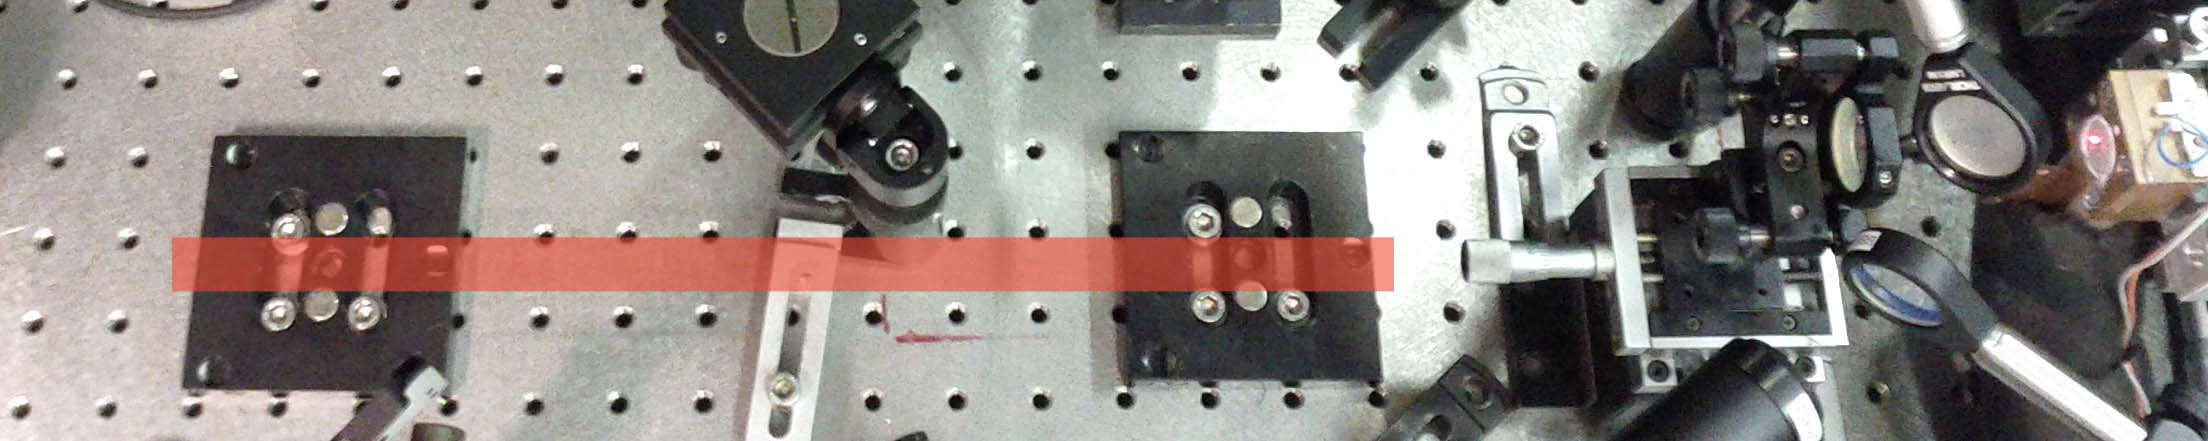
\includegraphics[width=12.5cm]{img/appendix/beamline_empty.jpg}}
\subfigure{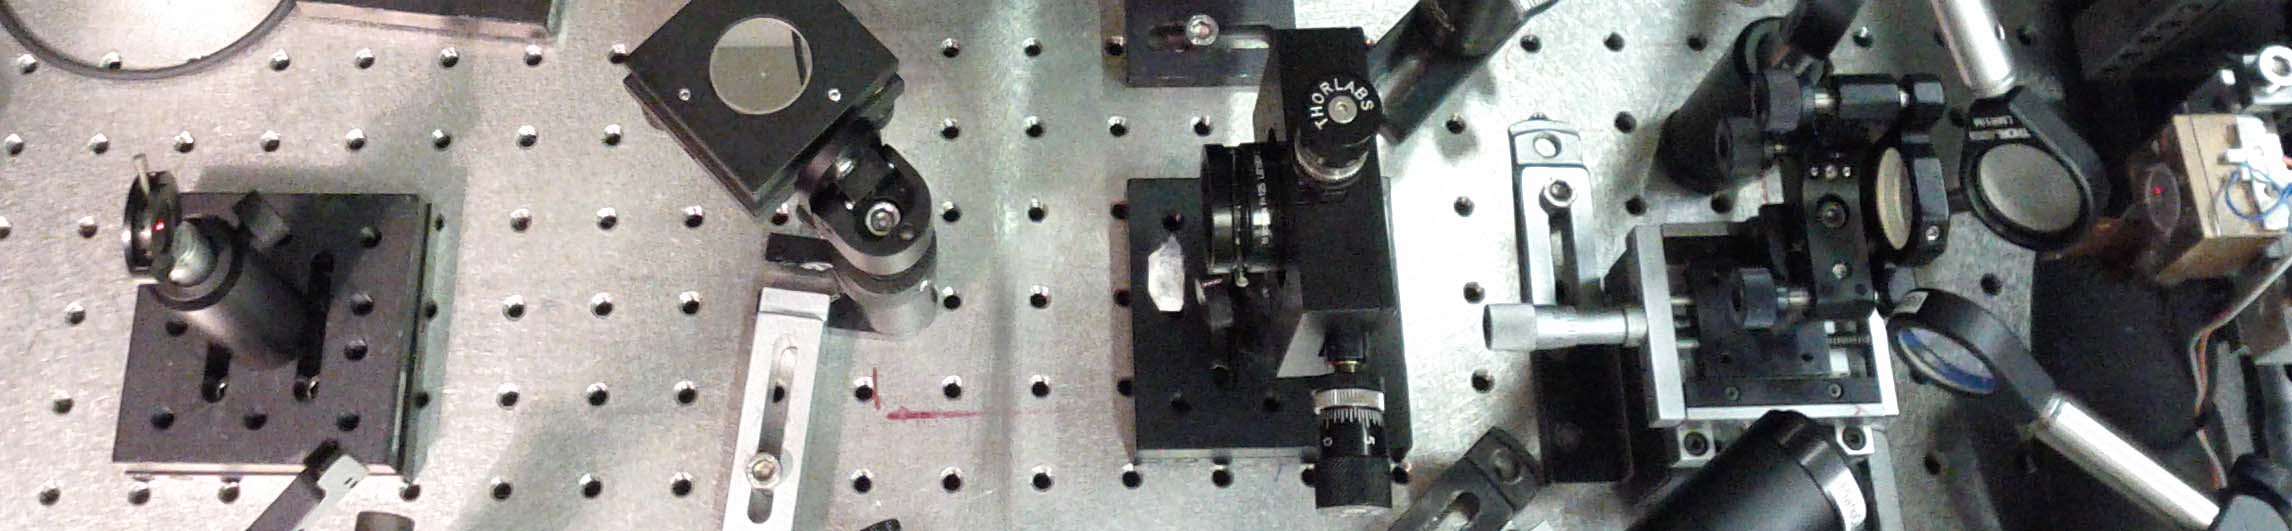
\includegraphics[width=12.5cm]{img/appendix/beamline_populated.jpg}}
\caption{Top: Removeable posts to define the beamline.
Bottom: HeNe beam has to be directed through the two irises.
With these two irises the position of the HeNe source is detached from the beam line.}
\label{img:beamline}
\end{figure}

In order to align the different parts we employ a HeNe laser.
Figure~\ref{img:beamline} shows the beam line orthogonal to the sample surface.
The beam line is defined by two removable magnetic posts.
These posts allow us to remove and replace a mount reproducible.
The beam line is ultimately defined by two irises.
As such, we can place the HeNe source anywhere on the table;
we simply have to guide its beam through these two irises.

For the alignment,
in a first stage,
we align the sample orthogonal to said beam line:
We remove -- or flip, Fig.~\ref{img:cavity_flipped} --
all other components along the beam line
and leave only the sample.
We adjust the orientation of the sample such that
the back-reflection is directed at the HeNe, Fig.~\ref{img:HeNe}.
Once the sample is aligned
we place the output coupler
back in the beam path
and repeat the same procedure.

\begin{figure}
\centering
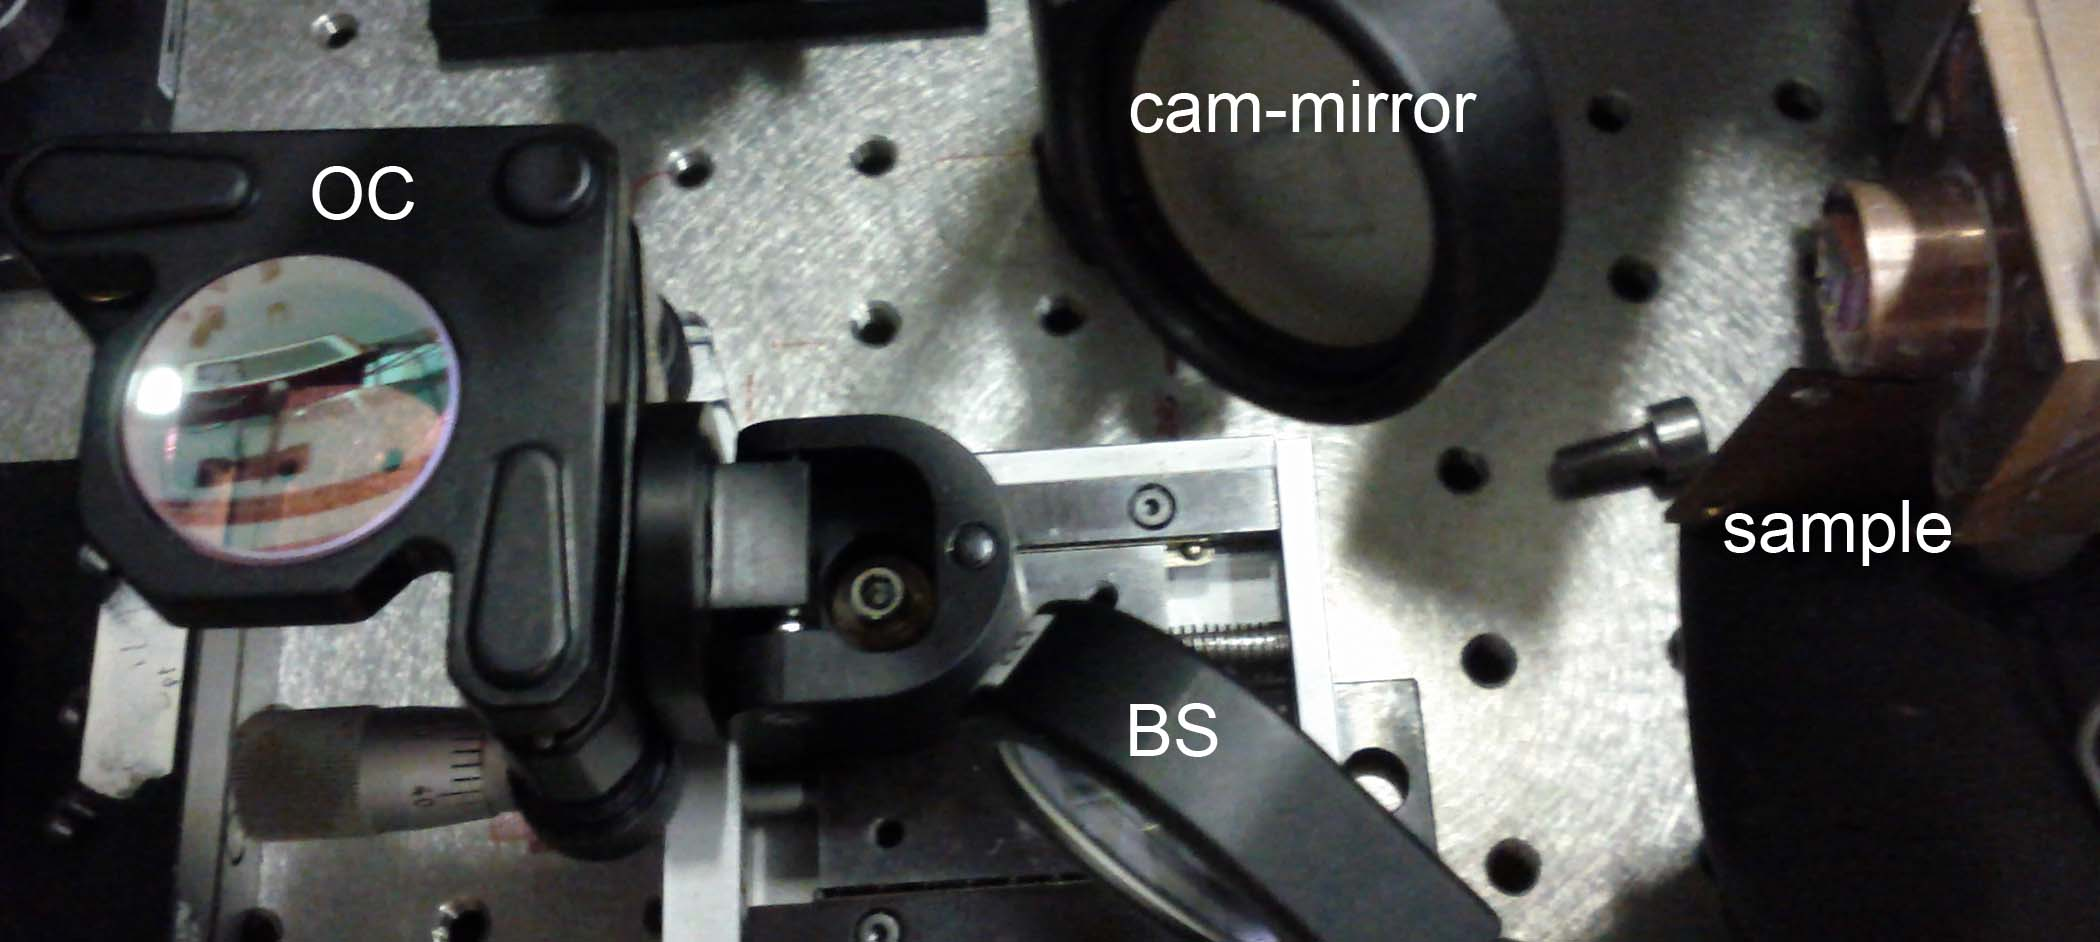
\includegraphics[width=12.5cm]{img/appendix/cavity_flipped.jpg}
\caption{First, we remove / flip all components along the beam line except the sample.
In this configuration we align the sample surface orthogonal to the HeNe.}
\label{img:cavity_flipped}
\end{figure}

\begin{figure}
\centering
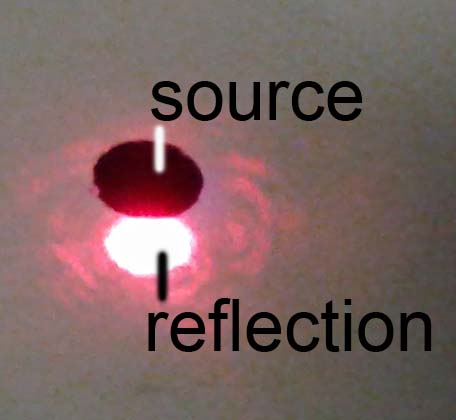
\includegraphics[width=4cm]{img/appendix/HeNe.jpg}
\caption{By arranging the reflected beam to coincide with the HeNe source position
we ensure the orthogonality of the component.}
\label{img:HeNe}
\end{figure}

In a last step we have to irradiate the sample with the 980~nm pump.
A camera along the emission beam line
sees the photoluminescence resulting from the pump on the sample.
This camera is equipped with a long-pass filter
in order to see only the photoluminescence
and not the pump light.
With this camera,
initially,
we see two spots corresponding to
pump and reflection from the output coupler.
Because of the aforementioned alignment with the HeNe laser
these two spots should already be close,
see Fig.~\ref{img:spot_overlap}.
We bring these two spots to overlap,
using the xyz-stage of the output coupler.
Once the two spots do overlap,
and the pump is above threshold,
the sample starts lasing.

\begin{figure}
\centering
\subfigure{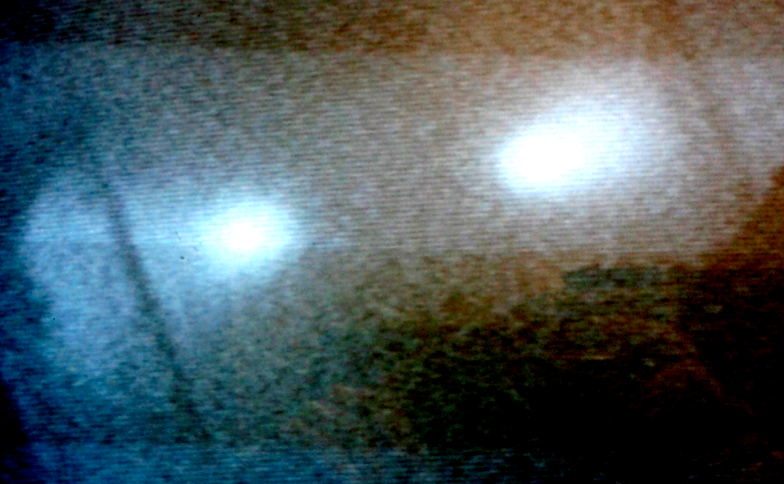
\includegraphics[width=6cm]{img/appendix/spot_overlap_two.png}}
\subfigure{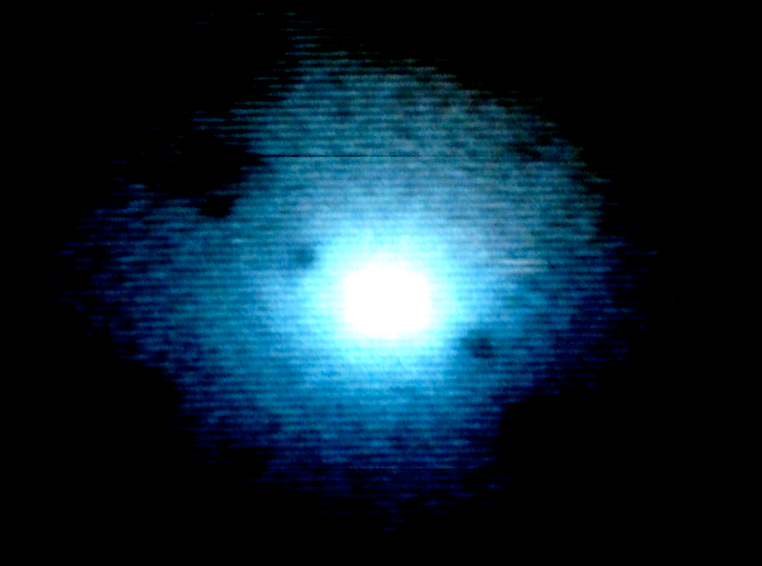
\includegraphics[width=6cm]{img/appendix/spot_overlap_one.png}}
\caption{After the pre-alignment
with the HeNe,
the two spots --
originating
from the pump
and the output coupler reflection --
are close by (left).
By optimizing the alignment
of the output coupler,
these two spots
have to be brought to overlap (right).
Given this configuration,
we have to increase the pump power,
and at threshold we obtain laser emission.
For the fine-alignment
we have to replace the camera
with a power meter
and adjust for maximum output power.}
\label{img:spot_overlap}
\end{figure}

Figure~\ref{img:overview} shows an overview of the different components.
The pump light is directed via fiber to a lens system that images the light onto the sample.
With beam sampler BS$_p$ we extract a fraction of the pump and direct it to detector det$_p$.
This way we have a realtime reading of the pumped power.
A considerable part of the pump light is reflected off the sample.
This light diverges.
First, we thus have to collimate it.
For this we install a lens with appropriate focal length and distance from the sample.
Of this reflected beam we again sample a fraction with BS$_r$,
and direct this to detector det$_r$.
The largest fraction of the reflected beam is directed to the beam dump.
By sampling pump and reflection in this geometry
we avoid high power readings on the detectors.

\begin{figure}
\centering
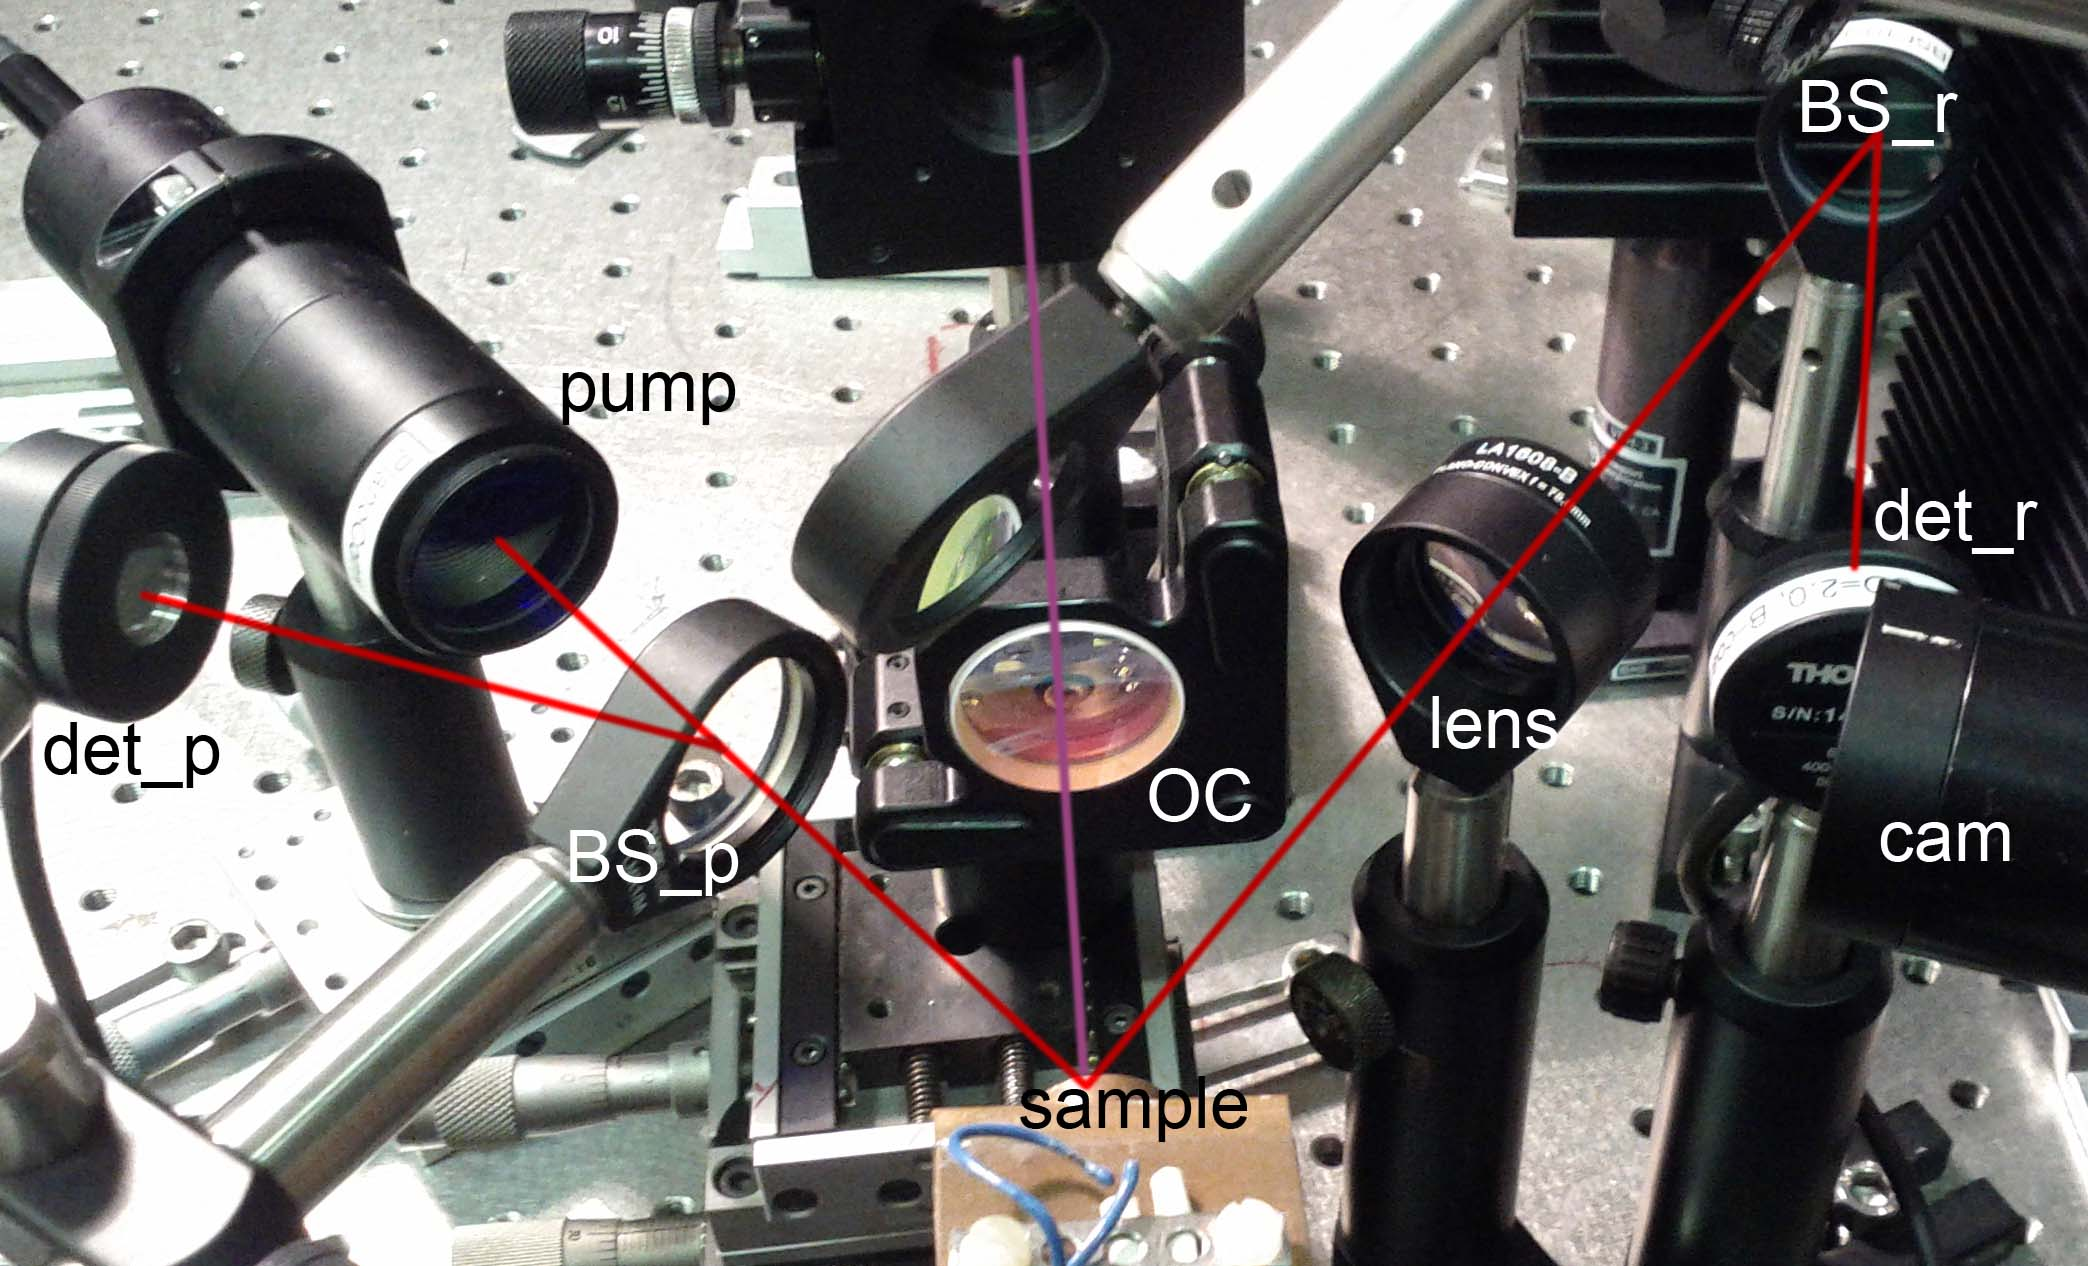
\includegraphics[width=12.5cm]{img/appendix/cavity_all.jpg}
\caption{Overview of the different components incorporated for the cavity.}
\label{img:overview}
\end{figure}





\section{Spatial filtering}
\label{app:spatial}

In the focal plane of a lens,
the intensity of the beam profile corresponds
to its Fourier transform.
To be more precise,
in the Fraunhofer approximation
(which is valid in the focal plane)
we find the intensity of each point on the focal plane
to be the amplitude of its respective
spacial Fourier component \cite{QE}.
We can use this fact
in order to manipulate the beam profile;
to spatially filter it.
This method is based on the fact that
Gaussians go into Gaussians under Fourier transform.

The core principle is simple:
We start with a (Gaussian) wave.
A first lens images this wave
onto the focal plane.
In this plane we place a mask.
This mask performs an operation
on the Fourier components present in the plane.
A second lens collimates the now modified beam back.

One useful mask geometry is a pinhole --
also known as low-pas filter.
Noise and other impurities on the beam profile,
picked up along the optical path,
is represented by higher Fourier components.
With a pinhole --
with appropriate aperture diameter --
we can cut off these higher components
and keep only the basic Gaussian in the middle.
Figure~\ref{img:spatialfiltering} by Edmund optics
illustrates this filtering.

\begin{figure}
\centering
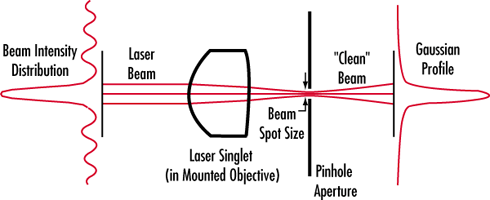
\includegraphics[width=12.5cm]{img/appendix/spatialfiltering.png}
\caption{Understanding Spatial Filters by Edmund optics \cite{Edmund}.}
\label{img:spatialfiltering}
\end{figure}

As already said,
the intensity in a point of the focal plane
is given by the amplitude
of its Fourier component $\nu_r$.
It is \cite{QE}
\begin{equation}
I = \left| \hat{g}(\nu_r) \right|^2,
\end{equation}
with $\hat{g}$ the Fourier transform
of a Gaussian beam
\begin{align}
g(r) &= \sqrt{I_0} \exp{\left(-\frac{r^2}{w_0^2}\right)}, \\
\hat{g}(\nu_r) &= \int r\d r\d \varphi g(r) \e^{i2\pi\nu_r r}\\
 &= \sqrt{I_0}\pi w_0^2 \exp{\left(-(\pi w_0 \nu_r)^2\right)}.
\end{align}
In the focal plane the Fourier component is given as
\begin{equation}
\nu_r = \frac{r}{\lambda f},
\end{equation}
with $\lambda$ the wavelength
and $f$ the focal length of the lens.
This results in an intensity distribution
\begin{equation}
I(r) = I_0(\pi w_0^2)^2 \exp{\left( -2(\frac{\pi w_0 r}{\lambda f})^2 \right)}.
\end{equation}
The fraction of power contained within diameter $D$ is hence \cite{Newport}
\begin{align}
\frac{P(r\leq \frac{D}{2})}{P_\mathrm{total}}
  &= \frac{2\pi}{P_\mathrm{total}} \int\limits_0^{D/2} I(r)r\d r \\
  &= 1- \exp{\left(-\frac{1}{2}(\frac{\pi w_0 D}{\lambda f})^2\right)}.
\label{eq:power}
\end{align}

A diameter of
\begin{equation}
D=\frac{f\lambda}{w_0}
\label{eq:diameter}
\end{equation}
permits $99.3\,\%$ of the total beam.
Newport \cite{Newport} recommends to use a pinhole
with this diameter.
Thorlabs on the other hand \cite{Thorlabs}
suggests to employ a pinhole
whose diameter is approximately $30\,\%$ larger.
The transmitted power in this case
would be $99.98\,\%$ of the total power.

By applying this method
to the output of a multi mode fiber,
we lose a considerable amount of this light;
the Gaussian part corresponds to TEM$_{0,0}$.
Starting with a Gaussian profile,
other methods can be used e.g.
to shape the beam into a super-Gaussian
\cite{Mansell2000},
in order to potentially
optimize the mode overlap.

\section{COMSOL implementation}
\label{app:comsol_deriv}

The commercial software COMSOL
allows us to perform thermal simulations
with a finite-element approach.
The heat equation
to be solved
reads as
\begin{equation}
0 = \nabla(k\nabla T) + Q.
\label{eq:app:heateq}
\end{equation}
It is $k$ the thermal conductivity of the material
($[k]=\mathrm{m}^{-1}$),
and $Q$ the heat source
($[Q]=\mathrm{W}/\mathrm{m}^3$);
originating from the pump beam.
Before we can talk about
the numerical insights
found with COMSOL,
we have to understand
the necessary parameters
and their influence
on this model.

\subsection{Heat source $Q$}
\label{app:comsol_deriv:Q}

In order to understand
how to investigate
the temperature distribution
within a VECSEL structure,
we have to understand
what input to provide to COMSOL
to solve the heat equation (\ref{eq:app:heateq}).
Our optical pumping represents
a heat source $Q$.
In this subsection
I present what this quantity looks like,
and what influence the different parameters --
most notably, the beam profile --
have.

The pump beam
is assumed to be
incident antiparallel to the $z$-axis
(here referred to as from the top).
We assume further
it is of Gaussian profile --
section~\ref{sec:comsol:beamprofile}
explains how to incorporate
different pump profiles.
In this configuration the heat source
associated with
each layer $j$ of the structure is given as
\cite{Kemp2008}
\begin{equation}
Q_j = \frac{2P}{\pi w^2} \eta_j\alpha_j \e^\frac{-2r^2}{w^2} \e^{-\alpha_j(z_{0j}-z)} \e^{-\sum_{i<j}\alpha_i t_i}.
\label{eq:app:heatsrc}
\end{equation}
The layers are counted from the top down --
the sum $\sum_{i<j}$ includes the layers on top
and ignores those below the layer of interest
(in that case $j$).
The meaning of the single parameters are listed in Tab.~\ref{tab:heatsrc}.
Furthermore we recognize
\begin{equation}
P'=P\e^{-\sum_{i<j}\alpha_i t_i}
\end{equation}
to represent the power still remaining after layer $1,2,\ldots,j$.
And
\begin{equation}
A=P'\eta_j
\end{equation}
corresponds
to the absorbed power in layer $j$;
which heats by factor $\alpha_j$.

\begin{table}[h]
\centering
\caption{Meaning of parameters used in (\ref{eq:app:heatsrc}).}
\begin{tabular}{llc}
\hline
Parameter & Explanation & Unit \\
\hline
$P$ & pump power & $\mathrm{W}$ \\
$w$ & pump beam $1/e^2$ radius & $\mathrm{m}$ \\
$\alpha_j$ & absorption coefficient of layer $j$ & $\mathrm{m}^{-1}$ \\
$r$ & radial coordinate & $\mathrm{m}$ \\
$z$ & axial coordinate & $\mathrm{m}$ \\
$z_{0j}$ & coordinate of top of layer $j$ & $\mathrm{m}$ \\
$t_j$ & thickness of layer $j$ & $\mathrm{m}$ \\
$\eta_j$ & heat loading fraction in layer $j$ & - \\
\hline
\end{tabular}
\label{tab:heatsrc}
\end{table}

The Gaussian beam assumed in (\ref{eq:app:heatsrc})
has an E-field \cite{QE}
\begin{equation}
E(r,z) \propto \frac{w_0}{w(z)} \exp(-\frac{r^2}{w^2(z)}) \exp(-i\Phi).
\label{eq:gaussE}
\end{equation}
The intensity of such a beam is proportional to the square modulus
\begin{align}
I(r,z) &\propto |E(r,z)|^2, \\
I(r,z) &= I_0 \left(\frac{w_0}{w(z)}\right)^2 \exp(-\frac{2r^2}{w^2(z)}).
\label{eq:gaussI}
\end{align}
This is where the factor $2$
in the exponent of (\ref{eq:app:heatsrc})
comes from.
The over all power
contained within the cross section
is constant, $P$.
Hence follows
the last part of (\ref{eq:app:heatsrc})
\begin{align}
P &= \int\limits_0^{2\pi}\d\varphi\int\limits_0^\infty r\d r I(r,z) \\
 &= 2\pi I_0 \left(\frac{w_0}{w(z)}\right)^2 \int\limits_0^\infty r \d r \exp(-\frac{2r^2}{w^2(z)}) \\
 &= 2\pi I_0 \left( \frac{w_0}{w(z)}\right)^2 \left[ -\frac{w^2(z)}{4} \exp(-\frac{2r^2}{w^2(z)}) \right]_0^\infty \\
 &= \frac{\pi}{2} w_0^2 I_0, \\
\Rightarrow\quad I_0 &= \frac{2P}{\pi w_0^2}.
\end{align}

\subsection{Implementation of our VECSEL structure}
\label{app:comsol_deriv:impl}

In this subsection I discuss the parameters
relevant for the actual COMSOL implementation,
taking our structure as an example
\cite{Ranta2014OptLett}.
A schematic of our VECSEL structure
is depicted in Fig.~\ref{img:design}.
Its fabrication details can be found in
\cite{Ranta2014OptLett,Sirbu2014SPIE}.
A summary of the used parameters --
in order to reproduce the presented results --
is given in appendix~\ref{app:comsolparams},
Tab.~\ref{tab:comsolparams}.

For the thermal conductivity
we have to consider
its spatial anisotropy.
The radial and axial thermal conductivity
we find with
\cite{Vetter2012,Lindberg2005,Osinski1993}
\begin{align}
k_r &= \frac{\sum_i k_i t_i}{\sum_i t_i} \\
k_z &= \frac{\sum_i t_i}{\sum_i \frac{t_i}{k_i}},
\label{eq:radaxthermcond}
\end{align}
with the actual values calculated from \cite{ioffe}
\begin{equation}
k_{\mathrm{Al}_{x}\mathrm{Ga}_{1-x}\mathrm{As}} =
0.55-2.12x+2.48x^2\,\mathrm{Wcm}^{-1}\mathrm{K}^{-1}.
\label{eq:k_AlGaAs}
\end{equation}
Before we employ
the extracted values of
a bulk Al$_{x}$Ga$_{1-x}$As material,
we divide them in half.
This way we account for
the empirically observed decrease
in thermal conductivity
in a layered structure such as a DBR
\cite{Piprek1998,Ranta2014APL}.

The absorption coefficient $\alpha_\mathrm{g}$ 
is chosen such that
it matches with the measured single pass absorption of $50\,\%$
\cite{Ranta2014OptLett}:
\begin{equation*}
\e^{-\alpha_\mathrm{g}t_\mathrm{g}}=0.5.
\end{equation*}

As a last important note we have to account
for the reflected beam:
it is absorbed in the gain section once again.
Hence we implement a second heat source in this gain layer
according to (\ref{eq:heatsrc})
\begin{equation}
Q_{\mathrm{g}_\mathrm{refl}} = \frac{2P}{\pi w^2} \eta_{\mathrm{g}_\mathrm{refl}}\alpha_g \e^\frac{-2r^2}{w^2} \e^{-\alpha_g(z_{0g}-t_g+z)}
 \e^{-\alpha_\mathrm{InP} t_c -\alpha_\mathrm{g} t_\mathrm{g} -2\alpha_\mathrm{InP}t_\mathrm{sp} -2\alpha_\mathrm{d}t_\mathrm{d}}.
\label{eq:heatsrcrefl}
\end{equation}
In this we have the expression
\begin{equation}
\eta_{\mathrm{g}_\mathrm{refl}} = \eta_\mathrm{g} (1-\eta_\mathrm{au}),
\label{eq:etagrefl}
\end{equation}
that assumes the fraction of reflected light
to be the residual light of what was not absorbed by the gold layer.
This remaining part heats the layer with efficiency $\eta_\mathrm{g}$.
Furthermore we see the sign in the exponent
\begin{equation*}
\e^{-\alpha_g(z_{0g}-t_g+z)}
\end{equation*}
to be positive.
This comes from the fact that in reflection
the beam travels in the opposite direction.

\subsection{Numeric convergence based on dimensionality}
\label{app:numconv}

\begin{figure}
\centering
\subfigure{\includegraphics[width=7cm]{img/appendix/r_HS-vs-T.png}}
\subfigure{\includegraphics[width=7cm]{img/appendix/r_v-vs-T.png}}
\caption{Left: Investigating on the convergence of the result,
depending on the system's dimension.
The size considered for the heat sink
is exponentially important.
Right: Investigating on the convergence of the result,
depending on the dimension of the VECSEL.
Considering a system larger than $2w_\mathrm{p}$
doesn't influence the over all result.}
\label{img:r_HS-r_v-vs-dT}
\end{figure}

Measuring the performance of a sample
in an experiment
is not the same as simulating it
numerically.
With COMSOL we can exploit
certain symmetries
imposed by the structure.
One is the radial symmetry
around an irradiated spot,
so that COMSOL has to solve
the equations only in two
rather than three dimensions --
which speeds up the calculations.
A second common simplification
is to simulate the VECSEL dimensions
only up to twice the size
of the pump spot \cite{Kemp2008}.
In order to ensure
such simplifications
don't lead to wrong conclusions,
we have to investigate
on the convergence behavior
depending on these parameters.
The names of parameters
are taken from
appendix~\ref{app:comsol_deriv:Q}--\ref{app:comsol_deriv:impl}
and Tab.~\ref{tab:comsolparams}.

Figure~\ref{img:r_HS-r_v-vs-dT} (left) presents
the convergence of the numerical result
depending on the system's size.
Each data point represents the following:
I simulate the temperature
on the surface of the structure
caused by a $P=32\,\mathrm{W}$,
$2w_p=300\,\mu\mathrm{m}$ pump diameter beam.
The radius of the VECSEL
is held constant at
$r_\mathrm{v}=2w_\mathrm{p}$.
In the center (at $r=0$)
the temperature is the highest;
this is the value we store,
for each system size $r_\mathrm{HS}$;
the considered radius of the heat sink.
For different values of $\eta_\mathrm{au}$
I look at various radii between
$r_\mathrm{HS}=1\,\mathrm{mm}$
and $r_\mathrm{HS}=5\,\mathrm{mm}$
(twice the size of our actual structure
with a cross section of $5\times5\,\mathrm{mm}^2$).
In the plot $\Delta T$ refers to the difference
between the temperature obtained with
the $r_\mathrm{HS}$ specified along the x-axis
and the temperature with $r_\mathrm{HS}=5\,\mathrm{mm}$.

The larger $r_\mathrm{HS}$ is chosen,
the less relevant is its actual value --
the temperature spread due to the extra bulk material
goes exponentially.
Therefore,
it seems to be important
to simulate the heat sink
(diamond layer and copper bulk)
as its full size.
The size of the VECSEL on the other hand
seems to be far less important;
its over all volume
and thus its ability to store and transfer heat
is small.
VESCEL sizes larger than two times the beam radius
result in the same temperature increase.
This statement is visualized
in Fig.~\ref{img:r_HS-r_v-vs-dT} (right).
In this plot,
the heat sink is kept
at constant $r_\mathrm{HS}=2.5\,\mathrm{mm}$ and
$r_\mathrm{v}$ is varied as multiples of $w_\mathrm{p}$.

The influence of the considered thickness of the gold layer
depends on whether or not
the incident beam is absorbed in this interface --
i.e. whether the gold layer only conducts the heat,
or is itself a heat source.
Figure~\ref{img:t_au-t_HS-vs-dT} (left)
illustrates this consideration.

\begin{figure}
\centering
\subfigure{\includegraphics[width=7cm]{img/appendix/t_au-vs-T.png}}
\subfigure{\includegraphics[width=7cm]{img/appendix/t_HS-vs-T.png}}
\caption{Left: Investigating on the convergence of the result,
depending on the thickness of the Au-Au bonding interface.
If we assume the gold layer
absorbs at least some of the incident beam,
we have to know the thickness of this layer.
Right: Investigating on the convergence of the result,
depending on the thickness of the copper heat sink considered.
Its importance depends on whether or not
we assume the gold layer to act as a heat source.}
\label{img:t_au-t_HS-vs-dT}
\end{figure}

In order to look at the influence of
the heat sink copper block
we assume
$r_\mathrm{HS}=2.5\,\mathrm{mm}$,
$r_\mathrm{v}=2w_\mathrm{p}$,
$t_\mathrm{au}=100\,\mathrm{nm}$.
The bottom boundary of the copper block
is held at constant temperature.
A thicker copper heat sink hence means
that the heat has to travel a longer distance.
As shown in Fig.~\ref{img:t_au-t_HS-vs-dT} (right)
this extra distance is relevant;
especially if we consider the gold layer
to act as a heat source.


\subsection{Explicit listing of simulation parameters}
\label{app:comsolparams}

Because numerical simulations are difficult to reproduce
when the used parameters are unknown,
the ones I used for section~\ref{sec:comsol}
are listed in Tab.~\ref{tab:comsolparams}.

\begin{table}[h]
\centering
\caption{Parameters used in the COMSOL simulation
reported in section~\ref{sec:comsol}.}
\begin{tabular}{lll}
\hline
 & Quantity & Value \\
\hline
$P_\mathrm{p}$ & Pump power & $32\,\mathrm{W}$ \\
$w_\mathrm{p}$ & Pump beam radius ($1/\e^2$) & $100\,\mathrm{\mu m}$ \\
$t_\mathrm{c}$ & Thickness cap [Specs] & $0.1017\,\mathrm{\mu m}$ \\
$t_\mathrm{g}$ & Thick. gain [Specs] & $0.7785\,\mathrm{\mu m}$ \\
$t_\mathrm{sp}$ & Thick. InP spacer [$\lambda$, Specs] & $0.4039\,\mathrm{\mu m}$ \\
$t_\mathrm{d}$ & Thick. DBR [Specs] & $5.0709\,\mathrm{\mu m}$ \\
$t_\mathrm{au}$ & Thick. Au layer [estimate] & $200\,\mathrm{nm}$ \\
$t_\mathrm{dia}$ & Thick. diamond layer & $0.3\,\mathrm{mm}$ \\
$t_\mathrm{HS}$ & Thick. copper heat sink & $3\,\mathrm{mm}$ \\
$k_\mathrm{InP}$ & Thermal conductivity InP \cite{Piprek2002} & $68\,\mathrm{W/(K\cdot m)}$ \\
$k_\mathrm{g}$ & Therm. cond. gain \cite{Piprek2002} & $4\,\mathrm{W/(K\cdot m)}$ \\
$k_\mathrm{d}$ & Therm. cond. DBR \cite{Piprek1998} & $0.35\,\mathrm{W/(cm\cdot K)}$ \\
$k_\mathrm{dr}$ & Therm. cond DBR in radial \cite{Vetter2012,ioffe,Piprek1998} & $36.8\,\mathrm{W/(m\cdot K)}$ \\
$k_\mathrm{dz}$ & Therm. cond DBR in z \cite{Vetter2012,ioffe,Piprek1998} & $34.6\,\mathrm{W/(m\cdot K)}$ \\
$k_\mathrm{dia}$ & Therm. cond. diamond \cite{Ranta2014OptLett} & $1800\,\mathrm{W/(m\cdot K)}$ \\
$k_\mathrm{au}$ & Therm. cond of gold \cite{SpringerMat} & $320\,\mathrm{W/(m\cdot K)}$ \\
$\alpha_\mathrm{InP}$ & Absorption coeff InP at 980 nm \cite{SpringerMat,ioffe} & $0\,\mathrm{mm}^{-1}\mathrm{}$ \\
$\alpha_\mathrm{g}$ & Absorpt. gain \cite{Ranta2014OptLett} & $0.9\times 10^{6}\,\mathrm{m}^{-1}\mathrm{}$ \\
$\alpha_\mathrm{d}$ & Abs. DBR at 980 nm \cite{SpringerMat,ioffe} & $0\,\mathrm{mm}^{-1}\mathrm{}$ \\
$\alpha_\mathrm{au}$ & Abs. Au \cite{SpringerMat,ioffe,Schubert} & $86554\,\mathrm{mm}^{-1}\mathrm{}$ \\
$\lambda_\mathrm{p}$ & Pump wavelength & $980\,\mathrm{nm}$ \\
$\lambda_\mathrm{L}$ & Laser wavelength & $1270\,\mathrm{nm}$ \\
$\eta_\mathrm{c}$ & Heat loading fraction: cap & $0$ \\
$\eta_\mathrm{g}$ & Heat loading fraction: gain & $1-\lambda_\mathrm{p}/\lambda_\mathrm{L}$ \\
$\eta_\mathrm{sp}$ & Heat loading fraction: spacer & $0$ \\
$\eta_\mathrm{d}$ & Heat loading fraction: DBR & $0$ \\
$\eta_\mathrm{au}$ & Heat loading fraction: Au & $0.75$ \\
$\eta_\mathrm{g_{refl}}$ & Heat load. frac.: Gain from reflected beam & $\eta_\mathrm{g}*(1-\eta_\mathrm{au})$ \\
$z_\mathrm{0c}$ & Coordinate top of cap & $z_\mathrm{0g}+t_\mathrm{c}$ \\
$z_\mathrm{0g}$ & Coord top of gain & $z_\mathrm{0sp}+t_\mathrm{g}$ \\
$z_\mathrm{0sp}$ & Coord top of spacer & $z_\mathrm{0d}+t_\mathrm{sp}$ \\
$z_\mathrm{0d}$ & Coord top of DBR & $z_\mathrm{0au}+t_\mathrm{d}$ \\
$z_\mathrm{0au}$ & Coord top Au layer; Interf. Au-DBR to be at 0. & $0\,\mathrm{m}$ \\
$z_\mathrm{dia}$ & Coord bottom diamon layer & $z_\mathrm{0au}-t_\mathrm{au}-t_\mathrm{dia}$ \\
$z_\mathrm{HS}$ & Coord bottom HS & $z_\mathrm{dia}-t_\mathrm{HS}$ \\
$r_\mathrm{v}$ & Width of VECSEL; small for better numeric & $2*w_\mathrm{p}$ \\
$r_\mathrm{HS}$ & Width of heat sink (and diamond) & $2.5\,\mathrm{mm}$ \\
$T_\mathrm{C}$ & \degr{0} & $273.16\,\mathrm{K}$ \\
$T_\mathrm{0}$ & Base temperature & $T_C+15\,\mathrm{K}$ \\
$\beta$ & Exponent of Supergaussian & $\{3,4\}$ \\
$a_\beta$ & normalization super-Gaussian & $\{0.5687,0.6267\}$ \\
\hline
\end{tabular}
\label{tab:comsolparams}
\end{table}


\newpage
\begin{thebibliography}{99}

\bibitem{Tropper2006}{A.~C.~Tropper, S.~Hoogland,
\textit{Review, Extended cavity surface-emitting semiconductor lasers},
Progress in Quantum Electronics 30, 1--43, (2006)}

\bibitem{Ranta2014OptLett}{A.~Rantam\"aki et al.,
\textit{High-power flip-chip semiconductor disk laser
in the 1.3 $\mu$m wavelength band},
Optics Letters, Vol. 39, No. 16, (2014)}

\bibitem{Kemp2008}{A.~J.~Kemp et al.,
\textit{Thermal Management in 2.3-$\mu$m Semiconductor Disk
Lasers: A Finite Element Analysis},
IEEE Journal of Quantum Electronics, Vol. 44, No. 2, (2008)}

\bibitem{Chernikov2010}{A.~Chernikov et al.,
\textit{Influence of the spatial pump distribution on
the performance of high power vertical-external-cavity surface-emitting
lasers},
Appl. Phys. Lett., vol. 97, no. 19, pp. 191110-1-191110-3, 2010}

\bibitem{Calvez2009}{S.~Calvez et al.,
\textit{Semiconductor disk lasers for the generation of visible and
ultraviolet radiation},
Laser \& Photon. Rev. 3, No. 5, 407--434 (2009)}

\bibitem{Sirbu2014OptExp}{A.~Sirbu et al., 
\textit{High performance wafer-fused semiconductor disk lasers
emitting in the 1300 nm waveband},
Optics Express, Vol. 22, Issue 24, pp. 29398-29403 (2014)}

\bibitem{Baili2009}{G.~Baili et al.,
\textit{Experimental demonstration of
a tunable dual-frequency semiconductor laser
free of relaxation oscillations},
Optics Letters, Vol. 34, No. 21, (2009)}

\bibitem{Lukowski2015}{M.~Lukowski et al.,
\textit{Widely Tunable High-Power Two-Color VECSELs
for New Wavelength Generation},
IEEE Journal of Selected Topics in Quantum Electronics,
Vol. 21, No. 1, (2015)}

\bibitem{Bedford2005}{R.~G.~Bedford et al.,
\textit{Power-limiting mechanisms in VECSELs}
in Proc. Enabling Photon. Technol.
Defense Security Aerospace Appl., (2005)}

\bibitem{Sirbu2014SPIE}{A.~Sirbu et al., 
\textit{Wafer-fused VECSELs emitting in the 1310 nm waveband},
Proc. SPIE 8966, 8966OG-1-8 (2014)}

\bibitem{Hader2011}{J.~Hader et al.,
\textit{VECSEL optimization using microscopic many-body physics},
IEEE J. Sel. Top. Quantum. Electron. 17, 1753 (2011)}

\bibitem{Kemp2005}{A.~J.~Kemp et al.,
\textit{Thermal Management in Vertical-External-Cavity
Surface-Emitting Lasers: Finite-Element
Analysis of a Heatspreader Approach},
IEEE Journal of Quantum Electronics, Vol. 41, No. 2, (2005)}

\bibitem{Heinen2012el}{B.~Heinen et al.,
\textit{106~W continuous-wave output power
from vertical-external-cavity surface-emitting laser},
Electron. Lett. 48, 516 (2012)}

\bibitem{Vetter2012}{S.~L.~Vetter, S.~C.~Calvez,
\textit{Thermal Management of Near-Infrared
Semiconductor Disk Lasers With AlGaAs Mirrors
and Lattice (Mis)Matched Active Regions},
IEEE Journal of Quantum Electronics, Vol. 48, No. 3, (2012)}

\bibitem{Devautour2013}{M.~Devautour et al., 
\textit{Thermal Management for High-Power Single-Frequency
Tunable Diode-Pumped VECSEL Emitting in the Near- and Mid-IR},
IEEE J. of Sel. Topics in Quant. El., Vol. 19, No. 4, (2013)}

\bibitem{Heinen2012}{B.~Heinen et al.,
\textit{On the Measurement of the Thermal Resistance
of Vertical-External-Cavity Surface-Emitting
Lasers (VECSELs)},
IEEE J. Quantum Electron. 48, 934 (2012)}

\bibitem{Giet2008}{S.~Giet et al.,
\textit{Comparison of thermal management techniques
for semiconductor disk lasers},
Proc. of SPIE Vol. 6871, 687115, (2008)}

\bibitem{Hader2013}{J.~Hader et al.,
\textit{On the measurement of the thermal impedance
in vertical-external-cavity surface-emitting lasers}
Journal of Applied Physics 113, 153102 (2013)}

\bibitem{Lindberg2005}{H.~Lindberg et al.,
\textit{Thermal Management of Optically Pumped
Long-Wavelength InP-Based Semiconductor
Disk Lasers},
IEEE Journal of Selected Topics in Quantum Electronics, Vol. 11, No. 5, (2005)}

\bibitem{Le1991}{H.~Q.~Le et al.,
\textit{Scalable high-power optically pumped GaAs laser}
App. Phy. Lett. 58, pp. 1967--1969, (1991)}

\bibitem{Korpi2010}{V.-M.~Korpij\"arvi et al.,
\textit{11 W single gain-chip dilute nitride disk laser
emitting around 1180 nm},
Optics Express, Vol. 18, No. 25, (2010)}

\bibitem{Nakwaski1992}{W.~Nakwaski and M.~Osinski,
\textit{Thermal resistance of top-surface-emitting vertical-cavity
semiconductor lasers and monolithic two-dimensional arrays}
Electronics Letters, 28(6), 72-574, (1992)}

\bibitem{ThorlabsAC}{Thorlabs,
\textit{Achromatic Doublets},\\
http://www.thorlabs.de/NewGroupPage9.cfm?ObjectGroup\_ID=259}

\bibitem{ThorlabsPM}{Thorlabs,
\textit{Power meter operation manual},\\
http://www.thorlabs.de/thorcat/19500/PM100USB-Manual.pdf}

\bibitem{Barlow}{R.~J.~Barlow,
\textit{Statistics -- A guide to the use of statistical methods
in the physical sciences},
The Manchester Physics Series,
Wiley, (1999)}

\bibitem{Efron1983}{B.~Efron, G.~Gong,
\textit{A Leisurely Look at the Bootstrap, the Jackknife and Cross-Validation},
The American Statistician, Vol 37, No 1 (Feb 1983), pp. 36-48}

\bibitem{Hessenius2011}{C.~Hessenius et al.,
\textit{Lateral lasing and ASE reduction in VECSELs},
in Proc. Vertical External Cavity Surface Emitting Lasers,
San Francisco, CA, 2011, pp. 791909-1-791909-8}

\bibitem{Chernikov2011}{A.~Chernikov et al.,
\textit{Heat management in high-power vertical-external-cavity
surface-emitting lasers},
IEEE J. Sel. Topics Quantum Electron., vol. 17,
no. 6, pp. 1772-1778, Nov.-Dec. 2011}

\bibitem{Mansell2000}{J.~D.~Mansell et al.,
\textit{Gaussian to Super-Gaussian Intensity Profile
Conversion with Refractive Micro-Optics},
online http://www.mansellassociates.com/CLEOTalk.pdf, (2000)}

\bibitem{Epperlein1993}{P.~W.~Epperlein,
\textit{Micro-temperature measurements on semiconductor laser
mirrors by reflectance modulation:
a newly developed technique for laser characterization},
Jpn.~J.~Appl.~Phys.~32, 5514-5522, (1993)}

\bibitem{Pierscinski2009}{K.~Pierscinski et al.,
\textit{Investigation of thermal management in optically pumped,
antimonide VECSELs},
Microelectron.~J., vol. 40, no. 3, pp. 558-561, (2009)}

\bibitem{Tessier2001}{G.~Tessier et al.,
\textit{Quantitative thermal imaging by synchronous
thermoreflectance with optimized illumination wavelengths},
Appl.~Phys.~Lett.~78, 2267-071106, (2001)}

\bibitem{SpringerMat}{Springer Materials,
\textit{The Landolt-B\"ornstein Database},
online http://www.springermaterials.com}

\bibitem{QE}{U.~Keller,
\textit{Lecture Quantum Electronics}, ETH Zurich, (2012)}

\bibitem{Edmund}{Edmund optics,
\textit{Understanding Spatial Filters},
online http://www.edmundoptics.de/technical-resources-center/lasers/understanding-spatial-filters}

\bibitem{Newport}{Newport,
\textit{Spatial Filters},
online http://www.newport.com/Spatial-Filters/144910/1033/content.aspx}

\bibitem{Thorlabs}{Thorlabs,
\textit{Principles of Spatial Filters},\\
http://www.thorlabs.de/NewGroupPage9.cfm?ObjectGroup\_ID=997}

\bibitem{Osinski1993}{M.~Osinski et al.,
\textit{Effective thermal conductivity analysis of
1.55 $\mu$m InGaAsP/InP vertical-cavity top-surface-emitting microlasers},
Electron. Lett., vol. 29, issue 11, (1993)}

\bibitem{ioffe}{Electronic Archive,
\textit{New Semiconductor Materials, Characteristics and
Properties},
online http://www.ioffe.ru/SVA/NSM/}

\bibitem{Piprek1998}{J.~Piprek et al.,
\textit{Thermal Conductivity Reduction in GaAs-AlAs
Distributed Bragg Reflectors},
IEEE Photonics Technology Letters, VOL. 10, NO. 1, (1998)}

\bibitem{Ranta2014APL}{A.~Rantam\"aki et al.,
\textit{High power semiconductor disk laser with a
semiconductor-dielectric-metal compound mirror},
Appl. Phys. Lett. 104, (2014)}







\bibitem{Piprek2002}{J.~Piprek et al.,
\textit{What Limits the Maximum Output Power of
Long-Wavelength AlGaInAs/InP Laser Diodes?},
IEEE Journal of Quantum Electronics, VOL. 38, NO. 9, (2002)}





\bibitem{Schubert}{E.~F.~Schubert,
\textit{Materials - Refractive index and extinction coefficient},
online http://homepages.rpi.edu/~schubert/Educational-resources/Materials-Refractive-index-and-extinction-coefficient.pdf,
Rensselaer Polytechnic Institute, NY USA}


\end{thebibliography}

\end{document}
